\documentclass{sfuthesis}

\title{Multi-scale investigation of snow accumulation on alpine glaciers}
\thesistype{Dissertation}
\author{Alexandra Pulwicki}
\previousdegrees{%
	B.Sc., University of Calgary, 2014}
\degree{Master of Science}
\discipline{Earth Science}
\department{Earth Science}
\faculty{Earth Science?}
\copyrightyear{2017}
\semester{Summer 2017}
\date{??}

\keywords{glacier; snow; spatial statistics}

\committee{%
	\chair{Pamela Isely}{Professor}
	\member{Gwenn Flowers}{Senior Supervisor\\Associate Professor}
	\member{Valentina Radic}{Committee Member\\Associate Professor}
	\member{Bonnibel Bubblegum}{Committee Member\\Associate Professor}
	\member{Hubert J.\ Farnsworth}{External Examiner\\Professor\\Department of Quantum Fields\\Mars University}
}

%   PACKAGES AND CUSTOMIZATIONS  %%%%%%%%%%%%%%%%%%%%%%%%

\usepackage{amsmath,amssymb,amsthm}
\usepackage[pdfborder={0 0 0}]{hyperref}
\usepackage{graphicx}
\usepackage{caption}
\usepackage{natbib}
\usepackage{wrapfig}
\usepackage{enumitem}
\setlist[enumerate]{itemsep=0mm}
\usepackage{multirow}
\usepackage{lscape}
\usepackage{caption}
\usepackage{subcaption}
\usepackage{float}
\usepackage{hyperref}
\usepackage{tabularx}
\usepackage{rotating}


\newcommand{\transectAbb}{Data for each glacier are divided into lower hourglass (LH), lower circle (LC), lower midline (LM), upper hourglass (UH), upper circle (UC), upper midline (UM), and upper transect (UT).}


%   FRONTMATTER  %%%%%%%%%%%%%%%%%%%%%%%%%%%%%%%%%%
\begin{document}

\frontmatter
\maketitle{}
\makecommittee{}

\begin{abstract}
	This is a blank document from which you can start writing your thesis.
\end{abstract}


\begin{dedication} % optional
\end{dedication}


\begin{acknowledgements} % optional
\end{acknowledgements}

\addtoToC{Table of Contents}\tableofcontents\clearpage
\addtoToC{List of Tables}\listoftables\clearpage
\addtoToC{List of Figures}\listoffigures





%   MAIN MATTER  %%%%%%%%%%%%%%%%%%%%%%%%%%%%%%%%%%%

\mainmatter%

\chapter{Literature review}

\section{Introduction}

Snow accumulation, as the dominant input of mass to alpine glaciers, plays an important role in governing their mass balance and the hydrology of alpine catchments more broadly. This has implications not only for the availability of water for local ecological and human use \citep{Barnett2005,ONeel2014}, but also for rates of global sea-level rise \citep{Gardner2013}. It is therefore necessary to understand the spatial distribution of snow on glaciers. However, achieving such an understanding is complicated by the fact that snow distribution in alpine regions is not uniform or static, but rather highly variable and influenced by diverse and dynamic processes operating on multiple spatial and temporal scales. Although previous research has attempted to account for these processes through the development of various techniques of measurement and modelling, little is known about how they operate in glacierized alpine environments. This severely limits possibilities of quantifying and predicting snow distribution on glaciers, particularly in remote locations where frequent empirical measurements are difficult \citep{Nolan2015}.

This proposal examines what is currently known and unknown about the topic of snow accumulation on glaciers and its spatial variability. The following section begins with an overview of accumulation variability within alpine regions in general, as there is a considerably greater breadth of studies devoted to snow in non-glacierized alpine basins. Section 3 reviews different ways of modelling the distribution of snow in alpine environments, while Section 4 describes methods for measuring accumulation and their relative merits and challenges. Section 5 compiles studies that specifically look at accumulation variability on glaciers and summarizes their key findings. Section 6 section focuses on the St. Elias Mountains, a large glacierized region where little is known about snow distribution and its effects on glacier mass balance. The final section described the proposed methodology for measurement of snow distribution in an area of the St. Elias Mountains and statistical techniques for the analysis of these observations. 

\section{Accumulation variability}

The spatial distribution of snow accumulation can vary significantly. This is a result of interactions between spatially and temporally variable atmospheric conditions and heterogeneous topography \citep{Deems2006, Liston2006}. Understanding and predicting snow distribution therefore requires accounting for factors that include atmospheric circulation, precipitable water, air pressure, air temperature, wind speed and direction, elevation, slope exposure, presence of orographic barriers, surface slope and aspect, surface roughness, and relief \citep{Schweizer2008a,McGrath2015}.

\subsection{Topographic scales}
Snow accumulation is spatially variable on point scales ($<$5 m), hillslope scales (1--100 m), watershed scales (100--10,000 m) and regional scales (10--1000 km) \citep{Clark2011}. The features and conditions that lead to variability at these scales differ (see Table \ref{scale}) and their relative importance depends on the topography and climate of the study area. Inclusion of parameters that describe relevant processes at multiple scales has been shown to improve models that aim to explain measured snow distribution \citep{Marchand2005, Clark2011}. 

Point-scale variability is generally associated with surface roughness effects and the presence of small obstacles. These effects can be significant in vegetated landscapes or when the surface is very rough (e.g. boulder field) \citep{Lopez2011}. Many parts of a glacier though are characterized by a relatively smooth surface, with roughness lengths on the order of centimeters \citep{Hock2005}. In these areas, point-scale variability of snow depth is low. However, in heavily crevassed regions, point-scale variability can be large and thus exert a dominant control on snow distribution in the area \citep{McGrath2015}. 

Hillslope-scale variability is caused by variations in the surface topography of the glacier. The curvature and slope of the surface as well as the presence of local ridges or depressions can affect where snow is located \citep{Bloeschl1999, Sold2013}. Avalanching can also redistribute snow, especially on the margins of a glacier \citep{Bloschl1991, Mott2008}. 

Watershed-scale variability results mainly from the effects of changing elevation and aspect on atmopsheric conditions \citep{Clark2011}. In particular, orographic lifting and shading can result in higher elevation and north-facing areas of the glacier having more snow than other areas \citep{Mott2008, Sold2013}. Gradients in temperature from elevation changes also affect the freezing level, which determines whether precipitation falls as snow or rain \citep{Bloschl1991}. For example, \cite{Machguth2006} found a strong influence of elevation in determining accumulation on Findel Glacier in Switzerland.

Regional variability occurs when areas within a mountain range have differing amounts of snow. Often, this results from horizontal precipitation gradients and rain shadows forming on the lee side of topographic divides. Areas with large, steep mountains are especially affected by these processes.

Generally, spatial variability increases with spatial scale \citep{Clark2011}. Extent and spacing of measurements must therefore capturing variability both across the study area and at smaller scales. \cite{Clark2011} note that studies of snow water equivalent (SWE) that have been conducted in alpine environments vary considerably in the extent and spacing of their measurements. 

\begin{table}[]
\centering
\caption{Relevant spatial scales for snow variability on glaciers. Information from \cite{Clark2011}.}
\label{scale}
\begin{tabular}{lll}
\textbf{Scale} & \textbf{Length} & \textbf{Associated glacier feature}                     \\ \hline
Point          & $<$5 m         & Crevasses                                               \\
Hillslope      & 1--100 m        & Local surface topography (curvature, slope), avalanching        \\
Watershed      & 100--10,000 m   & Elevation, aspect                                       \\
Regional       & 10--1000 km     & Horizontal precipitation gradient across mountain range
\end{tabular}
\end{table}

\subsection{Snow drift and preferential deposition}
Snow drift and preferential deposition are crucial factors that influence the distribution of snow \citep{Lehning2008, Winstral2002, Clark2011}. Sharp changes in topography cause convergent and divergent airflows close to the surface, leading to turbulence and vorticity. This terrain induced turbulence modifies mean wind (and snow particle) velocities, and can thus influence snow distribution via snow drift and/or preferential deposition \citep{Mott2008, Lehning2008, Dadic2010}.

Snow drift is the erosion and deposition of already deposited snow \citep{Dadic2010}. In general, erosion on the windward side is caused by increased wind speeds and deposition on the lee side of ridges is due to decreased wind speeds \citep{Liston1998, Mott2008, Dadic2010}. \cite{Mott2010} found that creep, which is the rolling of snow particles on the snow surface, and saltation, which is the bouncing and dislodging of snow particles, are primarily responsible for the formation of cornice-like features. 

Preferential deposition is inhomogeneous precipitation in the absence of local erosion \citep{Lehning2008}. It is mainly governed by winds, where higher wind velocities and updrafts on the windward side of ridges cause reduced deposition while reduced wind velocities on the lee side enhance deposition. This process can occur at relatively low wind speeds because it does not require the lifting of already deposited snow  --- instead, it only needs to act with or against the falling snow \citep{Mott2008, Dadic2010}. For example, \cite{Mott2011} found that the spatial structure of snow distribution in an alpine bowl was dominated by the preferential deposition of precipitation due to altered air flow fields. 

Both processes described can occur at multiple spatial scales. Enhanced accumulation has been observed on the point-scale in small depressions and on lee sides of obstacles, on the hillslope scale on the lee side of ridges, and at the watershed scale on sheltered aspects \citep{Harrison1986, Bloeschl1992, Mott2008, Winstral2002, Clark2011}. 

\section{Snow distribution models}
The distribution and variability of a parameter, such as snow water equivalent (SWE), can be estimated using either dynamic or statistical models. These models help to determine relevant processes that affect the distribution of snow, generally by relating its distribution to meteorological and topographic descriptors or conditions. Inferences made from these models drive the direction of future studies and provide valuable insight into understanding why variability arises. Accounting for wind in snow distribution models is especially important because it plays a dominant role in spatial patterns of accumulation \citep{Winstral2013}.

\subsection{Dynamic models}
Deposition and redistribution of snow can be represented using physically based, spatially distributed models. The general aim of these models is to simulate surface processes and how they vary spatially and temporally \citep{Mott2008}. These models usually consider atmospheric conditions including freezing level, precipitation rates, relative humidity, and wind speed and direction, as well as processes such as orographic lifting, cloud formation, downslope evaporation, advection and fallout, snow metamorphism, and wind redistribution of snow (erosion, saltation) due to terrain induced turbulence \citep{Smith2004, Liston2006, Lehning2008, Mott2008}.  Modelling the dynamically induced flows of these components together describes the preferential deposition and redistribution of snow in alpine environments \citep{Lehning2008,Mott2008,Dadic2010}.

Many models have been developed to describe preferential deposition and redistribution. Early models were developed for flat or gently rolling terrain where boundary layer flow is better understood \citep{Dadic2010}. Boundary layer flow in steep terrain is generally non-linear though \citep{Mott2008, Dadic2010}, so a number of different approaches have been applied.  For example, \cite{Dadic2010} and \citep{Lehning2008} solved non-hydrostatic, compressible Navier-Stokes equations in 3-D and aimed to conserve momentum, heat, mass, and states of water, to model wind flow velocities. \cite{Smith2004} employed Fourier transforms in a linear orographic model, which allowed for the more accurate representation of complex terrain. 

Dynamic models are a valuable way to determine accumulation variability. Since they use physically consistent processes, they can be applied to any site and generate values for each grid cell. They can also be used in different climatic conditions, allowing for predictions of accumulation change \citep{Clark2011}. Furthermore, a historic data set of variables is not needed to generate a meaningful output. Another advantage of dynamic models is that they allow for high temporal resolution (e.g. \cite{Mott2008} have a 1 hour time step), which allows for snowpack evolution to be examined.

Application of dynamic models is however operationally complex and computationally expensive, and also requires a diverse set of observations. Input parameters usually include temporally varying values for precipitation, wind speed and direction, air temperature, and relative humidity \citep{Liston2006}. Although these parameters can be obtained from meteorological stations, spatially distributed values --- found using atmospheric models --- are also required \citep{Liston2006, Mott2008}. For example, \cite{Dadic2010} used meteorological data from three automatic weather stations located throughout the study basin, while in the study done by \cite{Mott2008} monthly stake measurements were needed. Such a well-monitored basin can be difficult to achieve in remote or inaccessible areas. A number of other dynamic models, such as those described in \cite{Fowler2007}, use general circulation model (GCM) values to drive local circulation models, but it was shown that model output strongly depended on GCM boundary choice.  Even with sufficient and appropriate input data, the models must assume a number of parameters and simplify parameter relationships (e.g. constant mean wind speed \citep{Mott2008}) to characterize the atmosphere, which may not realistically describe air movement and stability. Additionally, the models do not account for all modes of snow transport. For example, snow deposition due to avalanching can be an important process of snow transport that is not captured in current models \citep{Mott2008}. 

\subsection{Statistical models}
Statistical models of snow variability establish empirical relationships between snow distribution and external variables \citep{Fowler2007}. These models assume that local distribution is forced by external factors, such a meteorological conditions or topography.

\subsubsection{Statistical downscaling}
Statistical downscaling is the process of determining an empirical relationship between large-scale atmospheric conditions and regional climates \citep{Fowler2007}. In general, this relationship is expressed as a function $F$ such that regional variables $R$ are found by $R=F(X)$ where $X$ encompasses large-scale climate variables \citep{Fowler2007}. These models are trained and validated using gridded reanalysis data from GCMs ($X$) and point observations ($R$). Performance of these models is measured using correlation coefficients, distance measures (e.g. root mean squared error), or explained variance \citep{Fowler2007}. 

There are three main types of statistical models \citep{Fowler2007}. The first is a regression model, which directly quantifies a relationship between a local variable and a number of large-scale variables. Statistical methods such as multiple linear regressions \citep{Hanssen-Bauer1998}, principal component analysis \citep{Kidson1998}, canonical-correlation analysis \citep{Busuioc2001}, neural networks \citep{Zorita1999}, and singular value decomposition \citep{Widmann2003} can be employed.  The second type of model is a weather typing scheme, which relates the occurrence of a particular `weather class' to local variables. Weather classes can be found using empirical orthogonal functions or cluster analysis \citep{Fowler2007}. The third model uses weather generators that simulate local precipitation occurrences with a chosen distribution of precipitation amount \citep{Fowler2007}. The large-scale input variables that are usually chosen (e.g. sea-level pressure, geopotential heights) for statistical downscaling are representative of large-scale circulation. Increasingly, other variables such as humidity are being incorporated into analyses to account for mechanisms that rely on thermodynamics and vapour content \citep{Fowler2007}. When focusing on precipitation, integrated vapour transport (IVT) can be used as a proxy for precipitable water in the atmosphere and can be used to identify corridors of large water vapour transport that correlate with intense precipitation events \citep{Neiman2008}. 

Statistical models are a simple way to examine variability. They are computationally efficient and comparatively easy to apply because they are based on standard and accepted statistical procedures \citep{Fowler2007}. Furthermore, generating values for specific point-scale variables does not require prior knowledge of all the processes that affect it. This allows for a function to be established for variables where all processes are currently not accounted for or where many processes are equally important. 

Although the application of statistical downscaling is simple, it has a number of disadvantages. The method is difficult to apply in areas that have a small amount of observed historical data, as model performance is better when a long and reliable data set is used for calibration  \citep{Fowler2007}. Statistical downscaling also assumes that the relationship between large-scale and local variables is stationary \citep{Fowler2007}. This means that use of the determined function is limited for projecting the variable of interest and further implies the need for long-term data observations. Furthermore, the empirical relationship assumes that there is no climate system feedback and the data generated through the empirical function are subject to the same biases as those of the original data set \citep{Fowler2007}. \cite{Wilby2000} also notes that the choice of large-scale variable domain (location and spatial extent) exerts a strong effect on the accuracy of the empirical function.

\subsubsection{Terrain-based parametrization}
Terrain-based parametrization is the linking of topographic indices determined from terrain modelling and observed conditions. To determine topographic indices, the terrain in the study area is divided into grid cells where terrain parameters (e.g. slope, curvature, aspect, ``northness'', wind exposure, topographic similarity) are calculated \citep{Anderson2014,McGrath2015}. The variable of interest is then measured in the study area and a relationship between grid-cell terrain parameters and observed data can be established \citep[e.g.][]{Bloschl1991, Liston1998, Anderton2004,McGrath2015}. 

This method requires a good terrain model and a meaningful network of observed data. For example, \cite{Molotch2005} found that that there were significant differences in modelled snow distribution when different terrain models were used. This is likely because the terrain-model grid size affects the value of the calculated terrain parameter for the cell. Terrain-based parameterization also needs sufficiently high resolution and spatial extent of the observed data. When measuring accumulation, the variability within the study area needs to be captured and all areas should be well represented. 

Relating terrain model parameters with observed data is often accomplished with simple statistical methods. Multiple linear regressions \citep{Marchand2005, Sold2013, McGrath2015}, mixed-effects multiple regression \citep{Kasurak2011}, parametric probability distributions \citep{Clark2011}, bivariate screening \citep{Anderton2004}, probability distribution functions \citep{Kerr2013}, and regression tree models \citep{Elder1998, Winstral2002, Molotch2005, Revuelto2014, Wetlaufer2016} are among the more popular models. These models statistically relate snow distribution to terrain parameters with varying success. For example, the multiple linear regression model developed by \cite{Sold2013} explained about 50$\%$ of the variance of snow depth while the model developed by \cite{Anderton2004} explained 70--80$\%$ of the variance in snow water equivalent. A number of studies have found that elevation and wind redistribution parameters explain the majority of the variance in observed snow depth or snow water equivalence \citep[e.g.][]{Erickson2005, Trujillo2009,Schirmer2011, Grunewald2014, McGrath2015}. Interaction parameters (e.g. $slope \times orientation$) have also been found to be significant predictors for precipitation distribution in alpine areas \citep{Basist1994}. \cite{Erxleben2002} and \cite{Molotch2005} note that many relationships between accumulation and controlling parameters are nonlinear so use of regression tree models yields better results. Combining statistical models has also been seen to improve model accuracy. Examples include combining linear regressions with generalized additive models \citep{Lopez2006} as well as binary decision trees with kriging \citep{Balk2000}. 

Relating topographic parameters and observed data is a simple approach to understanding processes that affect variability. Although no physically-based relations are employed, terrain parameters can act as proxies for processes that are known to occur \citep{McGrath2015}. In this way, dominant processes can be inferred through easy to find statistical relationships. This approach is especially powerful in areas such as alpine environments where topography strongly affects local conditions. 

While terrain-based parametrization is easy to employ, its usefulness in understanding snow distribution can be limited. This method assumes that variability between cells is larger than within cell variability, which may not necessarily apply to all cells, especially in steep terrain or where grid size is comparatively large. \cite{Marchand2005} found that the standard deviation within the 30 m by 30 m grid cells used in the study was slightly larger than the between-grid variability. Additionally, \cite{Grunewald2013} observed that local statistical models are able to perform well but that they cannot be transferred to different regions and that regional-scale models are not able to explain the majority of variance. The temporal transferability of terrain-based parameterization is also not reliable. \cite{Grunewald2013} found that local models could be applied between years while \cite{Revuelto2014} found that snow distribution variability could not be explained by their model in low snow years. Furthermore, the use of terrain parameters as proxies does not provide meaningful insight into relevant processes. This is important when attempting to predict distribution of variables in a different climate or location. 

\subsubsection{Variograms}
Length scales are distances over which data is correlated and they describe the degree of spatial dependence of a variable, which is likely due to a controlling processes. It is important to identify scaling processes of snow properties so that more effective models that account for processes at many scales can be developed \citep{Bloeschl1999, Deems2006a}. For example, the correlation length of snow depth can give insight into the effects of underlying topography and wind effects. The length scale of snow depth changes with time and is dependent on the amount of snow, influence of wind, and occurrence of melt. 

Geostatistical techniques and fractal analysis are the two main categories of tools that can be used to determine the length scale. Geostatitical techniques characterize a spatial pattern as composed of random deviations from a mean value and neglects any spatial structure that could exist in the random field \citep{Deems2006a}. These tools are used for distinguishing between autocorrelated and uncorrelated scale regions and have been widely used for snow science applications \citep[e.g][]{Bloeschl1999, Deems2006, Marshall2006}. Fractal analysis allows for stochastic structure within the random component and is able to identify multiple scales of variability \citep{Deems2006a}. Changes, or breaks, in variability scales are linked to important changes in processes that affect the observed spatial pattern. Fractal geometry (also known as scale invariance or self-similarity), has been observed in snow distribution patterns \citep{Shook1996, Granger2002, Deems2006a,Trujillo2007, Deems2008} and has been used to interpolate between snow depth observations \citep{Shook1997}.

The most traditional geospatial technique is to construct a variogram (or semivariogram), which is a plot of the variance between points at two locations (Figure \ref{variogram}(a)). The goal of the variogram is to estimate the autocorrelation structure of the underlying stochastic process. The semivariance $\gamma \left(h\right)$ is calculated by
\begin{equation}
\gamma(h) = \frac{1}{2\left| N(h) \right|}\sum_{N(h)} \left(z_i-z_j \right)^2 ,
\end{equation}
where $N(h)$ is the set of all pairwise Euclidean distances $i-j=h$, $\left|N(h)\right|$ is the number of distinct pairs of $N(h)$, and $z_i$ and $z_j$ are the data vales at spatial locations $i$ and $j$, respectively \citep{Schirmer2011a}. Variance will increase as the distance between points increases, indicating that the values at these points are increasingly less dependent on each other. The distance at which this value no longer increases is the correlation length (also called the range) and the variance at this point (random field) is referred to as the sill ($\lim_{h\to\infty}\gamma(h)$) \citep{Srivastava2013}. In practice, the correlation length exists only for stationary processes with a constant mean and is defined as the distance at which semivariance reaches 95\% \citep{Deems2006a}. Variability that was not captured in the measurement, due to insufficient sampling resolution and measurement error, is referred to at the nugget and is the y-intercept of a variogram. Data with a high degree of spatial structure will exhibit a steep slope for the sill is reached and data with low spatial structure would show a more gradual slope. Other analyses that present similar information to the semivariogram include autocorrelation and covariance.

Information from variograms is often used for interpolating point measurements to find spatial patterns. \cite{Reuter2016} claim that geostatistical methods are preferred over simple regressions for interpolating data because they incorporate spatial autocorrelation directly from measurements. Kriging is a commonly used interpolation technique that assigns weights for observed values based on the data covariance. There are many types of kriging, including ordinary, universal, block, and external drift, which have different assumptions about the mean of the data and include different components of the data (e.g. residuals) \citep{Webster2001}. 

\begin{figure}
\begin{minipage}[c][8cm][t]{.58\textwidth}
        \vspace*{\fill}
  \centering
  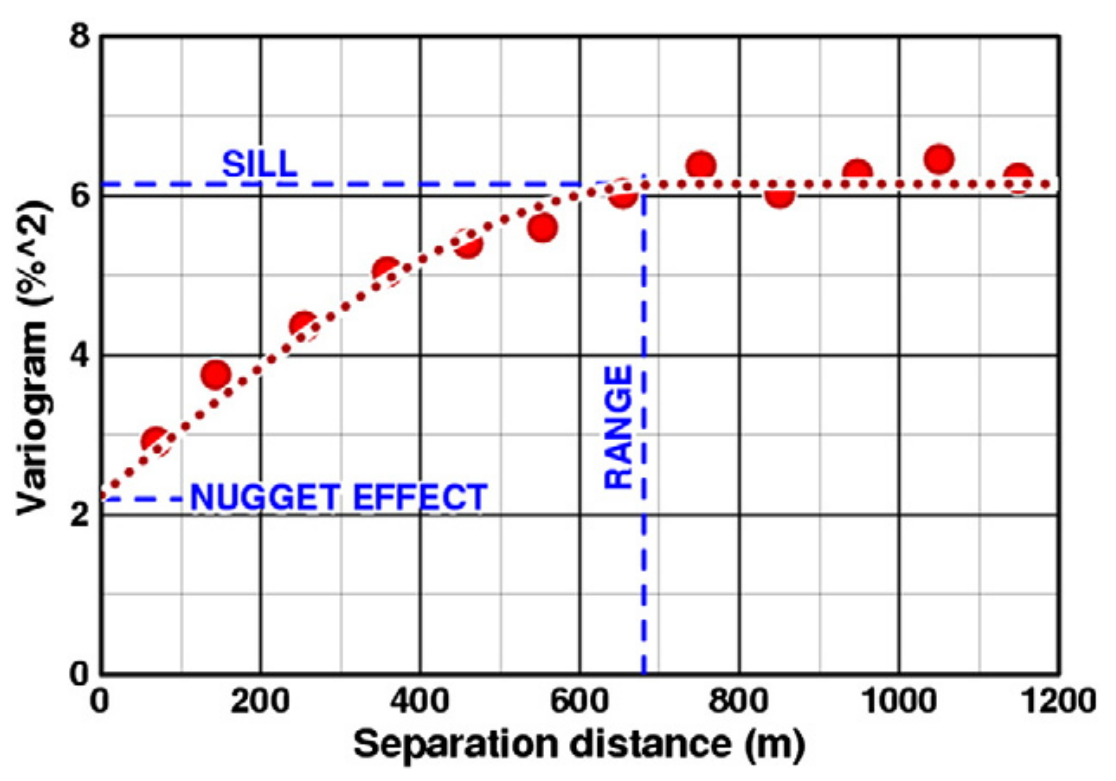
\includegraphics[height=6cm]{variogram.png}
  \subcaption{Variogram}
\end{minipage}%
\begin{minipage}[c][8cm][t]{.38\textwidth}
        \vspace*{\fill} 
          \centering
         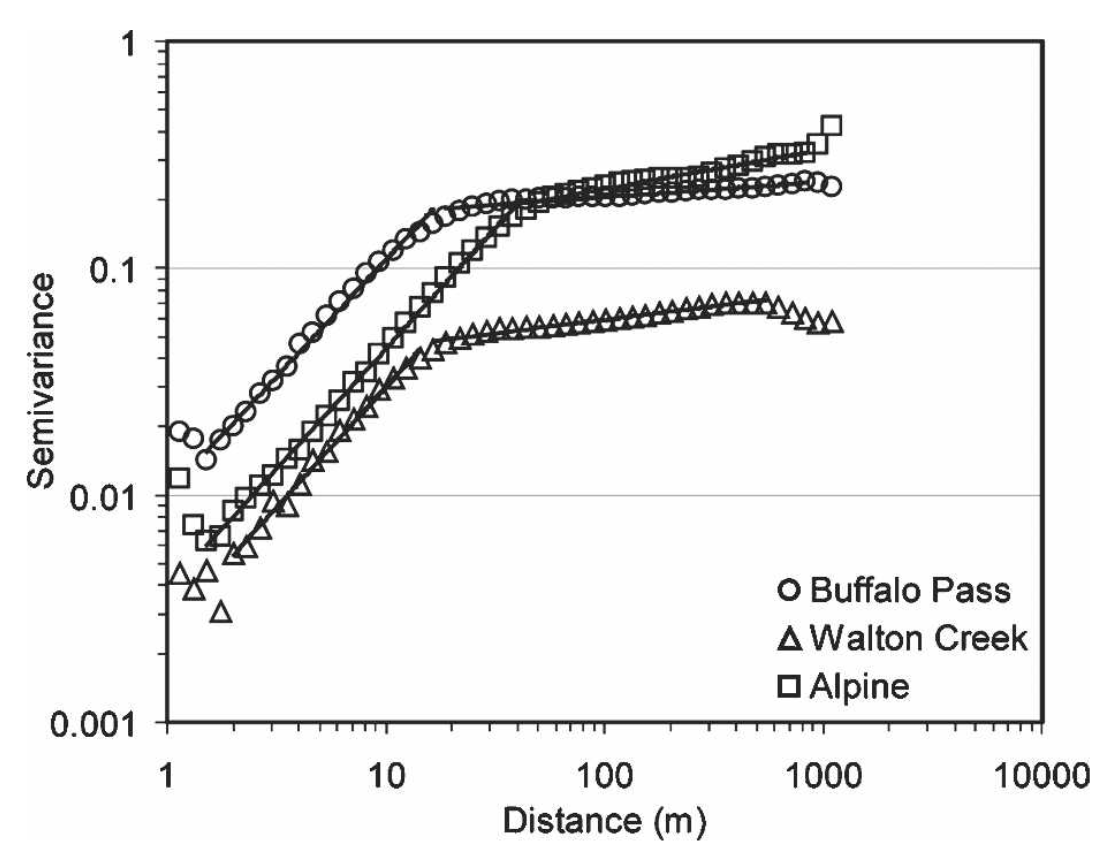
\includegraphics[height=5.5cm]{loglogvario.png}
  \subcaption{Log-log variogram}
  \end{minipage}%

\caption{Example of a variogram (from \cite{Srivastava2013}) and a log-log variogram with scale breaks (from \cite{Deems2006a}).}
\label{variogram}
\end{figure}

Fractal analysis attempts to identify scale-invariant spatial patterns, which means the observed variable has similar statistical properties at multiple scales. In this case, spatial pattern characteristics can be transferred from one scale to another using a scaling factor and this can also provide information about the scale, scope, and resolution of modelling and sampling efforts \citep{Deems2006a}. The most common way of identifying scale-invariance and scale breaks is by analyzing the slope of a log-transformed variogram (see Figure\ref{variogram} (b)), where log-linear segments indicate self-similar, fractal distributions \citep{Deems2006a}. For example, \cite{Schirmer2011a} used fractal analysis to confirm the effect of dominant wind direction on snow distribution by examining differences in scale break between windward, lee, and cross-loaded slopes. Power spectra (log-log plots) can also be used to examine scale-invariant patterns with the wave number and spectral exponent representing the spatial scale and degree of variability, respectively \citep{Trujillo2007, Trujillo2009}.

% Measuring accumulation
\section{Measuring accumulation}
Determining accumulation requires knowledge of snow density and depth. Measuring these parameters within a glacierized basin has many challenges. Basin location and topography affect accessibility, while the cost and time required to conduct measurements can be prohibitive. In most cases, the resolution of measurements over a large area is insufficient to approximate the true variability \citep{Bloeschl1999, Deems2006a}.

The chosen scientific question also guides choices in measurement tools and sampling design. Drivers of variability should be considered prior to sampling so that a sampling pattern is designed to capture this variability and to avoid sampling bias. When designing a snow survey, the support, spacing, and extent of the observations need to be defined \citep{Bloschl1995}. The support refers to the area or footprint of each measurement (tool dependent), the spacing is the distance between measurements, and the extent is the region that is being sampled. 

Snow density can be measured directly or with models of snow density change. To measure bulk density, a column of snow with a known volume is excavated (in a snow pit or with a firn corer) and weighed \citep{Sold2013, Sold2014}. Usually, a number of snow column densities are measured and the average density is taken as representative of glacier-wide density \citep[e.g.][]{Machguth2006, Grunewald2010, McGrath2015}. This can result in error when calculating snow water equivalence (SWE) because density can vary spatially and temporally (due to total snow depth, elevation, solar radiation, and wind effects) in a way that is not captured by a limited number of snow density measurements \citep{Grunewald2010, Wetlaufer2016}. However, snow density has been seen to vary over greater spatial scales than snow depth so fewer density measurements are usually made \citep{Elder1998, Clark2011}. Snow and firn density can also be calculated using models that account for relevant processes such as compaction from overlaying snow and refreezing of meltwater \citep{Herron1980, Sold2014}. Densification processes are difficult to capture in models though, so they should be applied with caution \citep{Mellor1974}.

Three main methods are currently used to measure snow depth. Probing involves taking \textit{in situ} point measurements of snow depth, GPR surveying involves using radar to detect the snow depth along continuous lines, and DEM subtraction involves taking the difference between the glacier surface at the end of the ablation and at the end of the accumulation seasons to find snow depth. Methods are selectively applied based on desired spatial resolution, cost effectiveness, and equipment availability. Each is prone to different sources of error and there is ongoing research to reconcile these approaches \citep{Sold2014}.  

\subsection{Snow probing}
\label{snowprobing}
\begin{wrapfigure}{R}{0.4\textwidth}
 \centering
      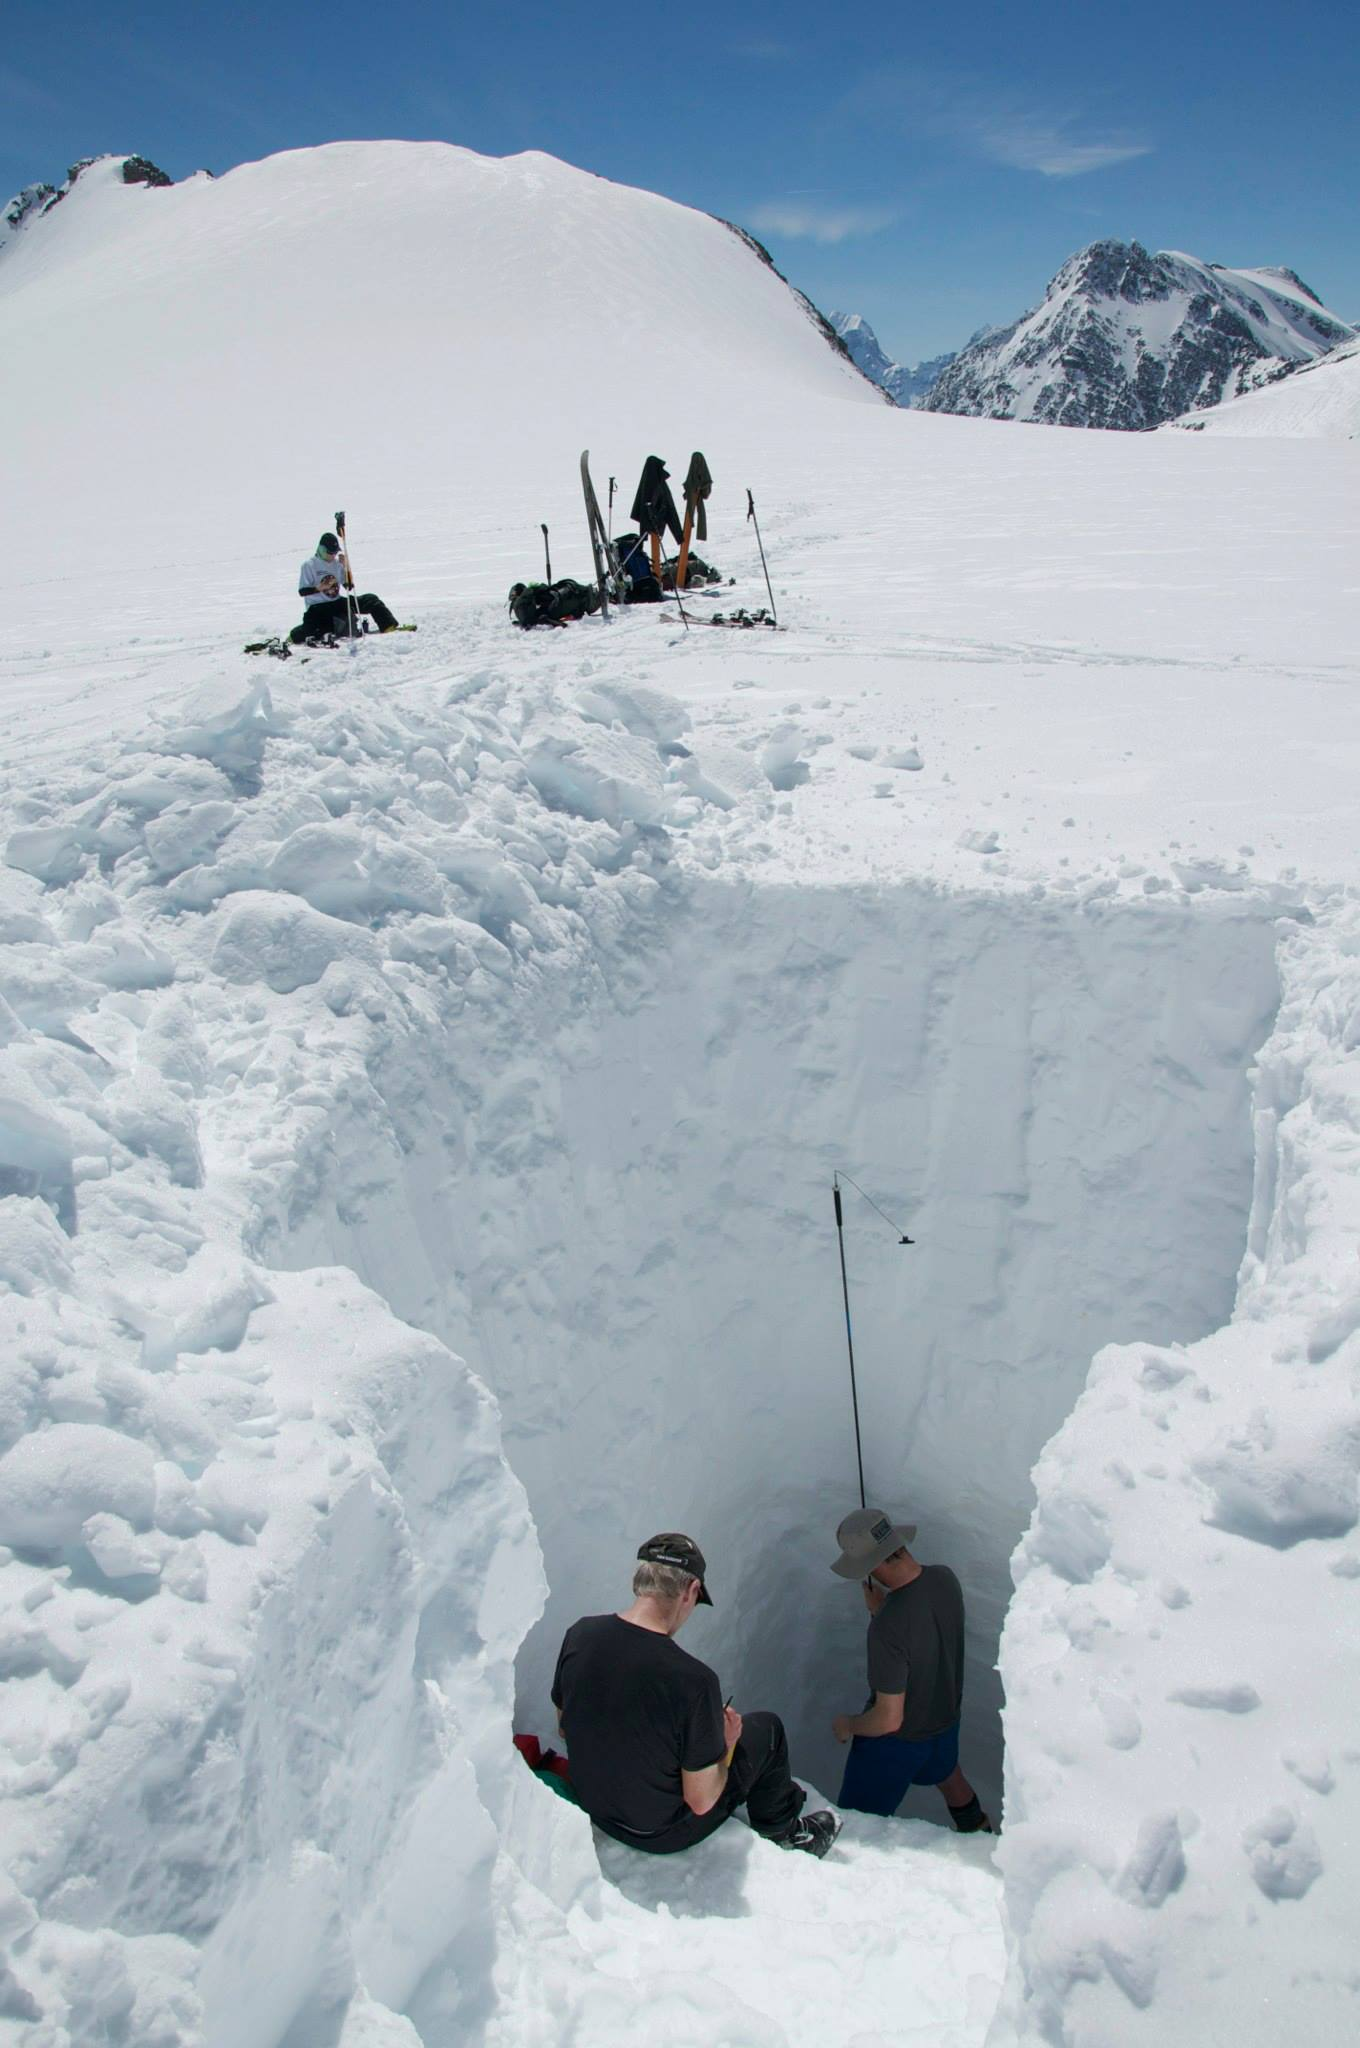
\includegraphics[width=0.4\textwidth]{snowpit.jpg}
  \caption{Digging a snowpit in the accumulation area of Haig Glacier, Rocky Mountains}
        \label{snowpit}
\end{wrapfigure}

\subsubsection{Measurement}
The most direct way of measuring snow depth is by probing. To determine the snowpack thickness, the height of the snow above the end of the previous year's ablation surface is measured. Usually, a number of snow height measurements are obtained close to each other and the mean value is taken to be representative of that location. For example, \cite{Machguth2006} took the mean of nine snow probe measurements within a 7 m radius as representative of a test site in the ablation zone.  

In the ablation zone, snow depth is easy to measure because the interface between the end of summer melt surface and the beginning of winter accumulation is well defined (i.e. glacier ice) \citep{McGrath2015}. In the accumulation zone however, the snow surface at the end of the melt season may not be easily distinguishable from the winter accumulation \citep{Grunewald2010}. It is common for the accumulation zone to have a heterogeneous surface at the end of the melt season --- some areas do not experience any melt,  while other areas experience some melt and the melt water percolates through the snow and firn. Melt water generated from warm weather or rain events, especially in the early and late parts of the accumulation season, can refreeze in the snowpack to form ice lenses \citep{Sold2014}. As a result, the interface can be difficult to observe and contain a combination of dense or compacted snow, ice lenses, and/or firn.  Probing in the accumulation zone can therefore result in erroneous depth measurements --- penetration into the dense snow or firn will make it seem like a deeper snowpack exists and probing to an ice lens within the snowpack can make it seem like shallower snow is present \citep{Sold2013}. Snow pits and firn cores are therefore used to examine snow and firn layers to determine where the current season's snow begins.

To determine the glacier-wide SWE, point snow depth measurements from probing need to be interpolated and extrapolated. This is often done using a statistical regression on parameters such as slope, aspect, curvature, and susceptibility to wind redistribution \citep[e.g.][]{Wheler2014,McGrath2015}. A regression generates an equation that is site specific and is used to estimate SWE for each grid cell based on the values of its relevant parameters. 

Snow probing is the simplest and oldest method used to determine accumulation. At the most basic level, it requires little more than a probe to determine depth, a way to determine location (such as a hand-held GPS), and a shovel to dig snow pits (see Figure \ref{snowpit}). Furthermore, this method directly measures snow depth so no data processing or corrections are needed and depth uncertainty is simple to quantify (often multiple depth measurements are taken close together) \citep{Sold2013}. 

There are however many drawbacks to this method. \textit{In situ} probing and digging snow pits are incredibly time-consuming \citep{Deems2006}. This limits the number of measurements that can be made, which means that accumulation measurements are under-represented and spatial variability in accumulation is difficult to capture \citep{Sold2014}. Measurement is also limited to areas that are both accessible and safe for researchers. In complex terrain many areas cannot be surveyed, resulting in data gaps. \cite{Sold2013} noted that this systematic bias can result in incorrect values of glacier-wide accumulation --- particularly because inaccessible areas such as cliffs and ridges have relatively shallow accumulations (due to wind erosion), while heavily crevassed areas can accumulate deep snow packs. 

\subsubsection{Sampling Design}

Optimal sampling schemes for snow probing are central for accurately estimating snow distribution and mass balance from \textit{in situ} measurements. Measuring snow depth and travelling between measurement locations is both time consuming and can disturb the snow so care must be taken to choose a sampling scheme that avoids bias, allow for the greatest variability to be measured, and minimize distance travelled \citep{Shea2010}. A design that maximizes accuracy and minimizes effort is therefore desired \citep{Elder1991} and both theoretical \citep{Trujillo2015} and applied \citep{Kronholm2004,Shea2010} investigations of various sampling designs have been pursued. There are a number of different designs that have been employed to obtain point measurements, including pure random, linear random, nested, gridded random, and gridded. 

A purely random distribution of points is favourable because it avoids all bias, has the best correlation with true distribution, and is likely to capture the most variability \citep{Kronholm2007, Shea2010}. Logistically though, it is difficult to successfully measure all points in the study area because some may be impossible to access and some may be disrupted during travel or measurement. This design often results in inefficient travelling routes, which decreases the number of possible point measurements. \cite{Elder1991} show a simple basin-wide random sample is a less optimal sampling scheme than a stratified random sample that accounts for known variation. One instance of a purely random sampling scheme can be seen in Figure \ref{schemes}(a). 

Linear-random sampling schemes impose a structure to traverse as much of the study area as possible but allow for a random distance between sampling points. An example of this scheme is the `star', created by \cite{Shea2010}. A significant advantage of this scheme is that it was designed to minimize distance travelled while still measuring snow properties in various orientations and various distances apart, which reduces bias. However, since the observer travels in straight transects there is still a potential to miss smaller features or ones that parallel the transects (spatial autocorrelation). \cite{Shea2010} used comparative Monte Carlo simulations to validate that the star scheme performs equivalently or better than other (more structured) sampling methods and that it converges to the true distribution as well as a purely random scheme. One instance of a linear-random sampling scheme can be seen in Figure \ref{schemes}(b). Linear-random sampling can also be done in an `hourglass' shape with an inscribed circle (referred to as an hourglass sampling scheme). As seen in Figure \ref{schemes}(f), this pattern allows sampling in all directions and captures a wide range of snow depths from the underlying snow distribution (Parr, C., 2016 personal communication).

\begin{figure}
\begin{minipage}[c][11cm][t]{.33\textwidth}
        \vspace*{\fill}
  \centering
  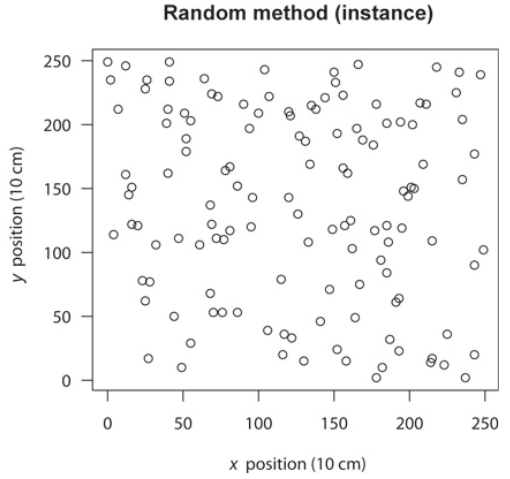
\includegraphics[width=5cm,height=4.5cm]{random.png}
  \subcaption{Pure random}
  \par\vfill
  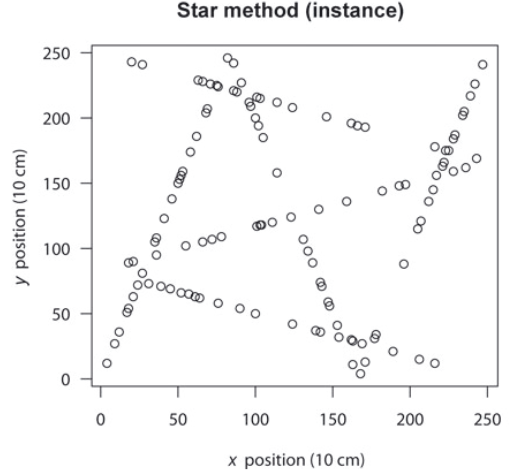
\includegraphics[width=5cm,height=4.5cm]{star.png}
  \subcaption{Star}
\end{minipage}%
\begin{minipage}[c][11cm][t]{.33\textwidth}
        \vspace*{\fill}
  \centering
  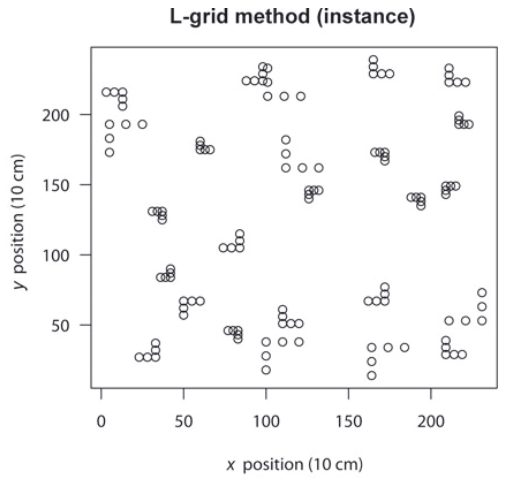
\includegraphics[width=5cm,height=4.5cm]{Lgrid.png}
  \subcaption{L-grid}
\par\vfill
  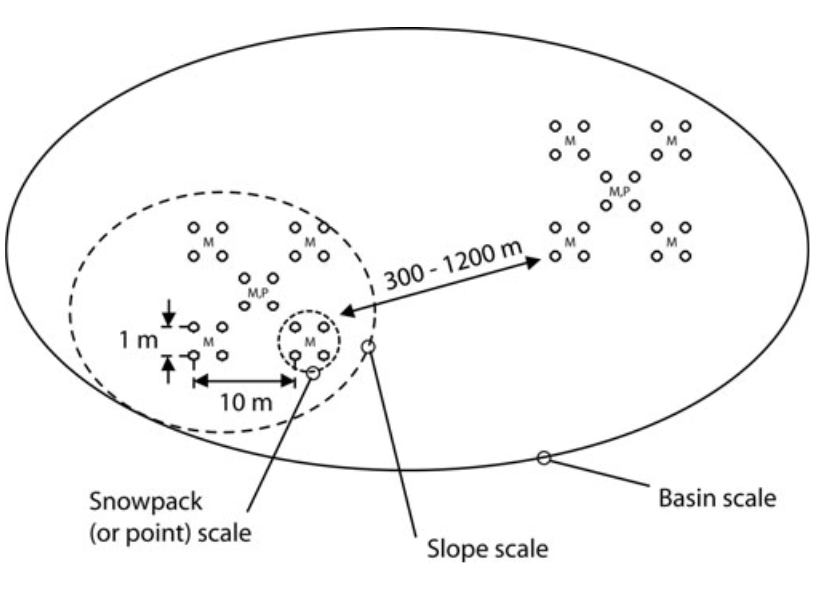
\includegraphics[width=5cm,height=4.5cm]{nested.png}
  \subcaption{Nested}
\end{minipage}%
\begin{minipage}[c][11cm][t]{.33\textwidth}
        \vspace*{\fill}
  \centering
    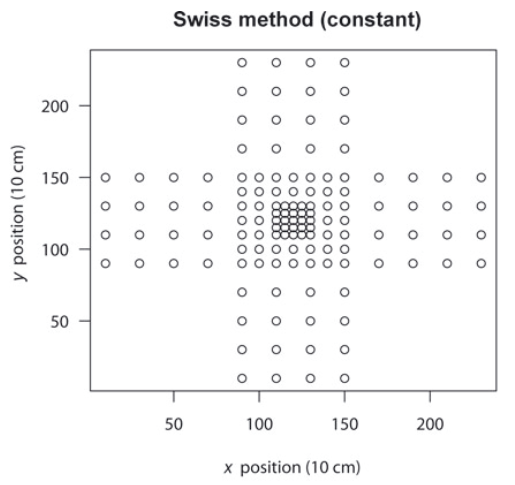
\includegraphics[width=5cm,height=4.5cm]{swiss.png}
  \subcaption{Swiss grid}
   \par\vfill
   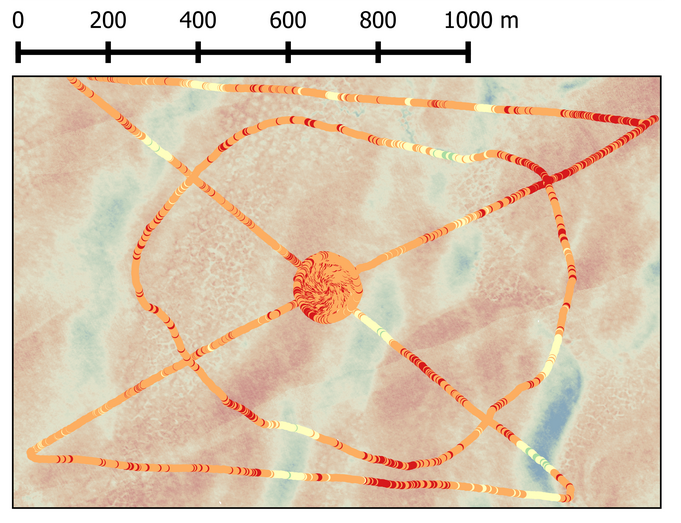
\includegraphics[width=5cm,height=4.5cm]{hourglass.png}
  \subcaption{Hourglass}
\end{minipage}
\caption{Examples of snow sampling schemes. Figures (a), (b), (c), and (e) from \cite{Shea2010}. Figure (d) from \cite{Schweizer2008}. Figure (f) from Parr, C., (2016 personal communication).}
\label{schemes}
\end{figure}

Gridded-random designs involve dividing the study area into equal sized areas and then sampling randomly within each area. The L-grid is an example of this scheme \citep{Bellaire2008, Elder2009, Bellaire2011}. In this scheme, the study area is divided into a grid and in each cell a random location is chosen as the start of the transect. The cardinal direction and measurement spacing of the transect are chosen randomly. Transects consist of five measurements, with three in the first direction selected and two perpendicular to this, forming an `L' shape. This scheme has a small error bias (maintains randomness), while allowing for more efficient measurement \citep{Shea2010}. Compared to the star scheme, the L-grid does not have a consistent travel distance and involves constant reorientation and finding of transect start locations, which decreases its efficiency. One instance of a gridded-random sampling scheme can be seen in Figure \ref{schemes}(c). 

Nested sampling is a scheme that maintains a certain sampling pattern and applies it at various length scales. For example, \cite{Schweizer2008} took four point measurement in a 1 m square and did this 10 m apart to form another square. The set of measurements was then repeated 300--1200 m away to capture basin scale values. Hierarchal trees that incorporate selected parameters are often used to determine nested sampling locations. \cite{Watson2006} and \cite{Kasurak2011} use hierarchal sampling to divide the study area into regions (often discontinuous) that are likely to have a similar snow distribution and low variance, which means they require lower density sampling. Nested sampling requires that the observer predetermine parameters that affect the spatial pattern of the variable. Often, remote sensing is used to obtain these parameters so the resolution of regions is limited to that of the remote sensing images (typically 30 m resolution). The variability that exists at scales less than the grid-size of the images is classified as being caused by `random' effects, which are assumed to be unbiased and unpredictable \citep{Watson2006}. Nested sampling is well suited for regions with many complex and interacting parameters. For example, \cite{Watson2006} used a hierarchal tree with time (traveling between locations), elevation, vegetation, and solar radiation at various length scales to create subgroup to sample.  A nested sampling scheme can be seen in Figure \ref{schemes}(d). 

Gridded sampling designs use regular measurement intervals in a grid pattern. Many variations of this scheme exist \citep{Molotch2005a, Kronholm2007, Lopez2011} with the most popular one being the Swiss cross \citep{Kronholm2004}. This nested arrangement allows for a larger area to be covered than a fully quadratic grid and measures at various spatial scales, leading to more reliable geospatial statistics. This method allows for easy measurement and reveals details at various scales. However, measurements are biased by regular spaced intervals and linear orientation, which could result in an under representation of the snow distribution further from the centre. A gridded sampling scheme can be seen in Figure \ref{schemes}(e). 

\subsection{GPR}
\begin{wrapfigure}{L}{0.5\textwidth}
 \centering
      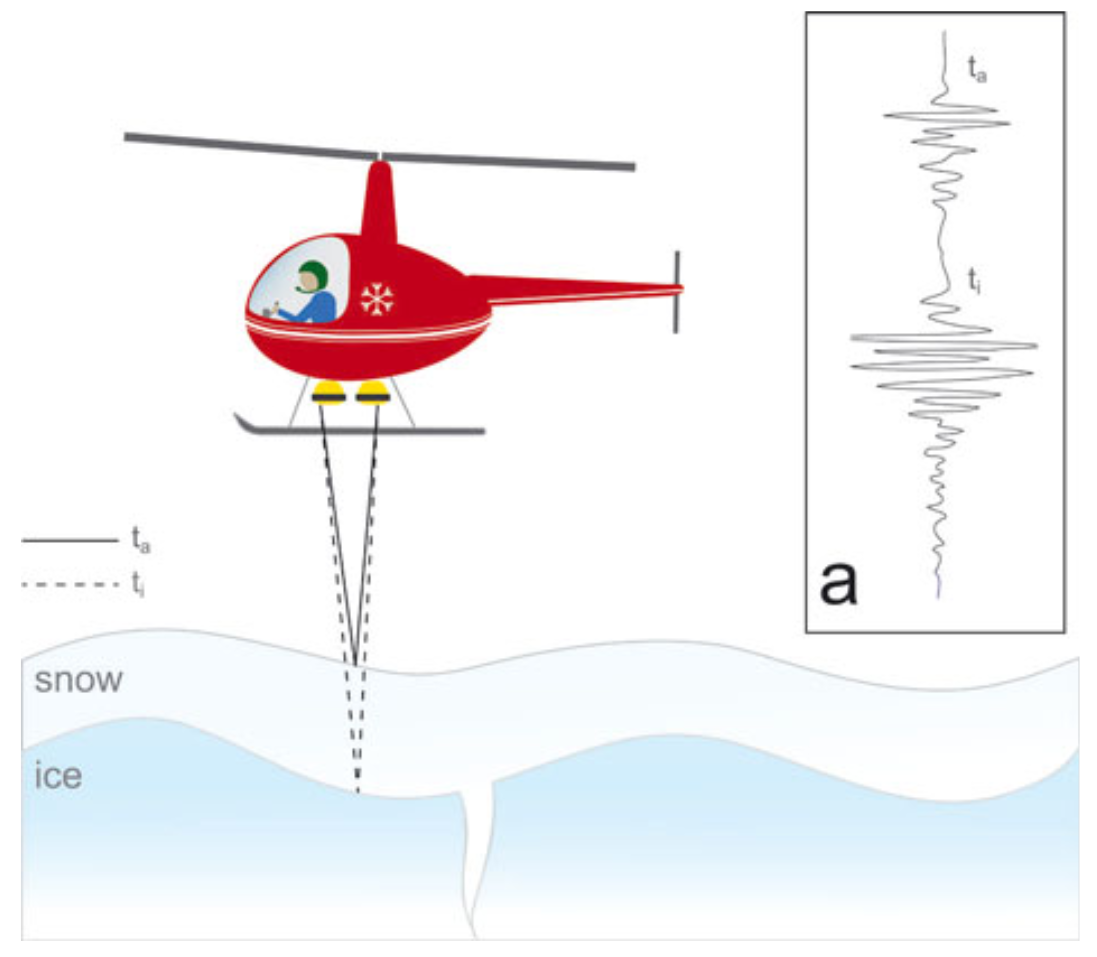
\includegraphics[width=0.5\textwidth]{gpr_air.png}
  \caption{Schematic diagram of a helicopter-borne radar snow survey. The travel time for the signal to interact with the snow surface is shown as a solid line and the signal travel time of the interaction with the ice is shown as a dashed line. Together, these values can be used to determine snow depth. The inset (a) is an example waveform that would be recorded from these two events. Figure taken from \cite{Gusmeroli2014}.}
        \label{gprair}
\end{wrapfigure}

Ground penetrating radar (GPR) can be used to find snow depth along continuous lines. This method is used to calculate the distance from the radar source to a boundary with a strong contrast in dielectric permittivity, which corresponds to a change in material properties \citep{Sold2013}. When the speed of the radar wave through the material is known, the travel time can be measured and from this the distance calculated. On a glacier, the radar wave is able to penetrate snow and ice at MHz frequencies and the strongest reflections arise when water is present \citep{Sold2013}. To measure snow depth, GPR units are mounted on aircrafts or snowmobiles that then travel over snow covered areas (see Figure \ref{gprair}) \citep{Machguth2006, McGrath2015}. The resulting processed radargram (e.g. Figure \ref{gpr}) gives a continuous snow depth profile. Processing of the radargrams involves using tracking algorithms that are able to trace continuous layers. Interpolation between transects is then done to find the glacier-wide accumulation. \cite{McGrath2015} describe this process in five steps: (i) acquisition of GPR and probing data (ground truthing), (ii) calculation of snow density and radar velocity, (iii) calculation of snow thickness and resulting SWE, (iv) application of a correction to measured accumulation based on ground truth data, and (v) use of a multiple regression model to extrapolate SWE across the glacier. The extrapolation of SWE can also be done using an inverse approach with a coupled surface energy-balance snow model \citep{Pelt2014}.

GPR is an effective tool for measuring accumulation. It provides continuous snow depth transects, which means that spatial variability is well represented along the radar lines. Surveys also need be conducted only once to gain depth observations, which makes data collection fast and and reduces logistical efforts\citep{Machguth2006}. GPR snow depth estimates are not affected by glacier dynamics and the ability to fly over steep or inaccessible regions means that all areas of a glacier can be measured. 

A large limitation of GPR is the difficultly of processing radargrams. Areas where the snow--ice boundary is not well defined (i.e. the accumulation area) lack clearly contrasted material properties, which can lead to misinterpretation of their internal layers \citep{McGrath2015}. In the ablation area, the presence of crevasses can also result in radargram misinterpretation \citep{Machguth2006}. Variation and uncertainty in radar wave speed due to differing snow density and liquid water content can also affect depth calculations \citep{Sold2013}. Often, wave speed is only measured in a few reference locations so changes in snow pack properties cannot be accounted for. Lastly, there is no universal procedure for processing GPR data. Selection of parameters and processing algorithms is dependent on available equipment, field conditions, survey design and intention \citep{Sold2013}, which hampers the reproducibility of surveys.

\begin{figure}
 \centering
      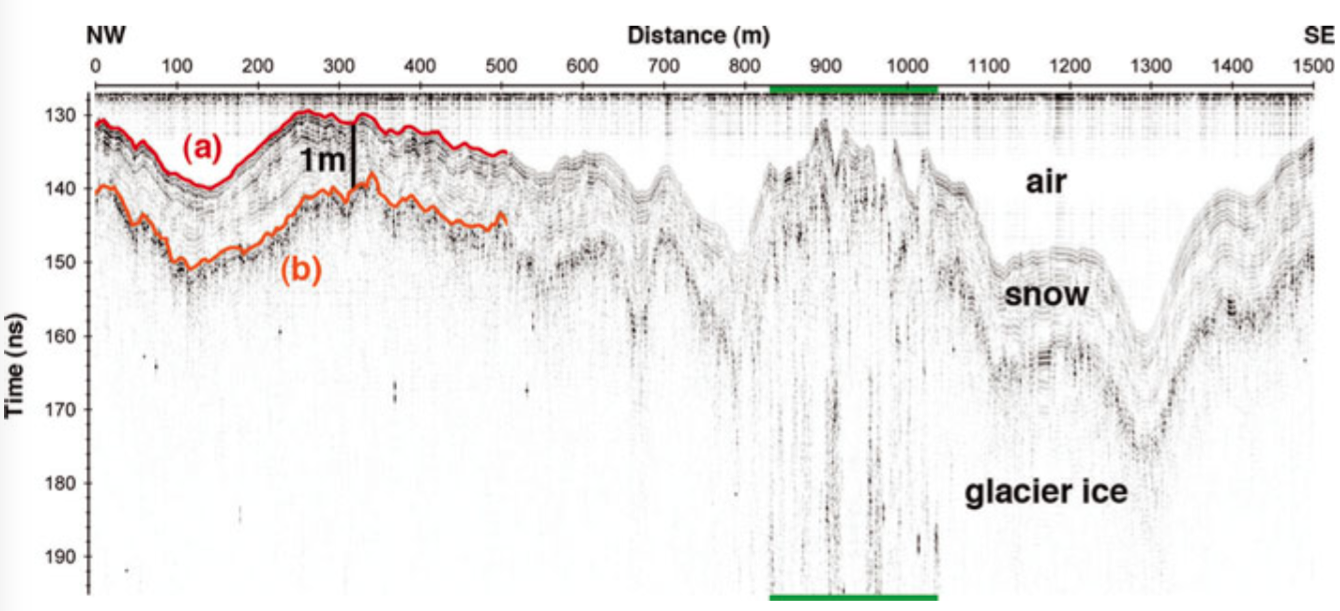
\includegraphics[width=\textwidth]{gpr.png}
  \caption{Radargram from the accumulation area of Findelengletscher, Valais, Switzerland. (a) The reflection at the air-snow interface. (b) The reflection at the snow-ice interface. Figure taken from \cite{Sold2013}.}
        \label{gpr}
\end{figure}

\subsection{DEM subtraction}
\begin{wrapfigure}{R}{0.5\textwidth}
 \centering
      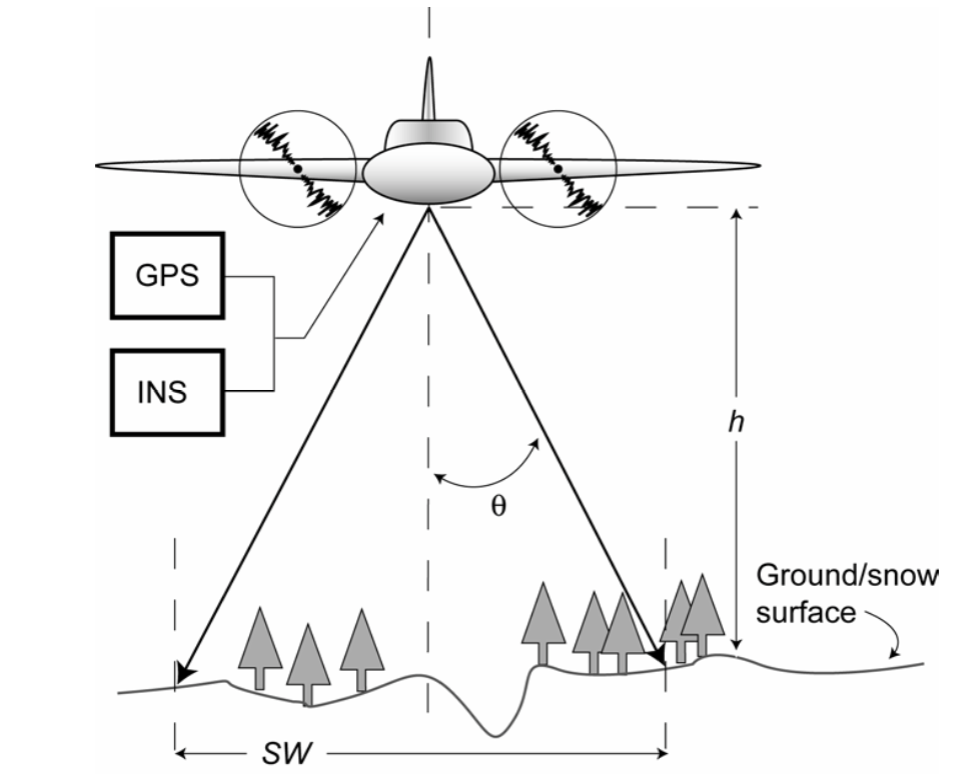
\includegraphics[width=0.5\textwidth]{lidar.png}
  \caption{Schematic of airborne LiDAR system geometry. Scan angle ($\theta$), height ($h$), and swath width ($SW$) are shown. Figure from \cite{Deems2006}.}
        \label{lidar}
\end{wrapfigure}

Digital elevation model (DEM) subtraction involves taking two detailed surface topography scans --- one at the end of the melt season and one at the end of the accumulation season --- and subtracting them from each other to find the snowpack height. The largest advantage of this remote sensing method is that it provides a highly resolved spatial measurement of snow depth over an entire basin \citep{Deems2006, Sold2013}. Data collection is fast, although two surveys must be conducted. This technique is sensitive to other processes that change the glacier surface elevation, including vertical displacement due to ice flow (positive in the ablation area and negative in the accumulation area), firn compaction, and surface lowering due to melt after the acquisition of the end of melt season DEM \citep{Sold2013}. For example, \citep{Sold2013} found that a first-order approach (where the observed elevation change was interpreted as snow accumulation) was inconsistent with snow depth probing --- DEM subtraction showed decreasing accumulation with an increase in elevation. Corrections can be made to account for these discrepancies but they rely on \textit{in situ} measurement of snow depth, knowledge of long-term mass balance, or information about the vertical displacement of ice from GPS towers \citep{Sold2013}. 

Lidar and photogrammetry are the two main methods of producing DEMs. Lidar produces a surface elevation model by calculating the distance to a target (by measuring the time between an emitted and return laser signal) \citep{Deems2006, Sold2013}. Terrestrial lidar systems involve stationary units placed in vantage points from which they are able to scan the basin surface \citep{Grunewald2010}. Large basins require multiple overlapping scans to acquire a complete surface profile. Airborne lidar systems (see Figure \ref{lidar}) can also only scan a certain size footprint so the aircraft must fly over all parts of the basin to acquire a full surface profile. These systems also require an accurate global positioning system (GPS) --- which is often corrected by referencing to a stationary GPS --- to determine the 3D locations of the surface \citep{Deems2006}. Airborne systems are widely applied and favourable in large basins or ones where no vantage point exists or is inaccessible. However, these systems are expensive so terrestrial scanners, which are comparatively more cost effective, are becoming popular \citep{Grunewald2010}. 

Complex topography and multiple laser reflections can cause problems when producing a DEM from lidar data \citep{Deems2006}. Significant vertical changes result in the spreading of the laser footprint and an incorrect interpretation of distance. \citep{Deems2006} shows that an error of 50 cm can result from lidar scans of 45$^\circ$ terrain from 1000 m flight height. Careful planning of flight paths can reduce this error. Scattering of laser light and penetration into the snow pack can also introduce error into height calculations, although its magnitude is small ($\sim$cm) \citep{Deems2006}. When subtracting the two measured DEMs, misclassification of corresponding point locations can occur, resulting in error in the final accumulation value \citep{Deems2006}.  

Photogrammetry uses photographs to produce a series of DEMs that can be subtracted to find snow depth. Early attempts in the 1960s at applying this technique in snow covered areas suffered from poor vertical resolution due to overexposed photographs and the necessity of manual differencing \citep{Nolan2015}. Modern photography equipment, GPS, and software technology have allowed for an increase in accuracy and lowering of costs associated with photogrammetry \citep{Nolan2015}. Current photogrammetry software is able to determine a snow surface profile relative to stable, snow-free points within the mapped area \citep{Farinotti2010}. The photos collected for DEM creation can also be used to identify suspect changes in the snow pack \citep{Nolan2015}.
Errors in photogrammetric measurements arise from sensor noise and poor lighting. Camera sensor noise is present in all digital photographs and its location changes from picture to picture. These erroneous pixels can be misinterpreted by the software as actual differences in height and thus lead to significant topographic noise, especially in steep mountainous terrain \citep{Nolan2015}. Additionally, having sufficient contrast in the photographed snow surface is critical for determining surface profile. Flat light conditions can reduce the resolution of the DEM or result in an absence of data in those parts of the photograph \citep{Nolan2015}. These effects can be avoided by waiting for better lighting. 

\subsection{Comparison of methods}
\label{sec:comparemethods}
The three methods of measuring accumulation differ in the extent of spatial information, collection techniques and costs, and processing needs. Spatial footprint is lowest for probing, which means that data must be interpolated. Although the actual measurement is simple and has relatively low uncertainty, the interpolation of points can lead to misrepresentation of spatial variability and significant errors that are not quantified. GPR provides continuous snow depth profiles, but interpolation is still needed between lines. Further, significant errors can arise from interpretation of layers in radargrams. DEM differencing has the advantage of allowing for the measurement of surface topography across the whole basin, but error can result when glacier dynamics affect surface height changes and in the conversion between snow height and to water equivalent. 

Large differences in data collection time and cost also exist. Probing has low equipment costs but requires a large amount of human hours for ground-based measurements. GPR and DEM subtraction both require the use of aircrafts and expensive electronic equipment. However, these methods require lower logistical effort and data collection occurs quickly.  

The three methods also have different data processing requirements. Simple statistical relations can be used for interpolating accumulation found by probing. However, GPR and DEM subtraction both require specialized software and knowledge of image processing methods, which increases the likelihood that misinterpretations of observations will occur. GPR has an advantage over DEM subtraction because it is not subject to elevation changes due to glacier dynamics and firn compaction. However, DEM subtraction has the advantage of more easily detecting the previous year's surface in the accumulation area and provides complete coverage of the study area \citep{Sold2013}. 

In general, \cite{Machguth2006} and \cite{Sold2013} found good correlations between probing measurements, GPR, and DEM subtraction. However, \citep{Sold2013} found that the methods did not always corroborate each other, particularly in crevassed areas and marginal regions. In crevassed areas, accumulation has large variation on small scales. The footprint of the GPR was usually too large to detect changes in snow depth and the movement of crevasses with time affected the lidar-derived snow depth. Marginal regions were misrepresented in the probing-derived profile because measurement was often not conducted in these areas (Section \ref{snowprobing}). This area also included the uppermost part of the glacier where wind erosion had a significant effect on accumulation. 

Choice of measurement technique for a snow survey is therefore dependent on project specific needs. Resolution, cost, and equipment availability need to be considered when selecting the most appropriate method. To reduce errors and misrepresentation of measurements, multiple methods can also be applied \citep{Machguth2006}. 

\subsection{Temporally resolved methods}
Temporally resolved methods measure accumulation continuously to provide a time series of snow accumulation. Usually, these methods involve relatively sparse point measurements so they do not represent spatial variability well. However, they are especially useful for identifying large snowfall events (rapid increases in accumulation) and wind erosion (gradual decreases in accumulation). 

There are a number of methods of measuring SWE with time. Snow depth sensors, such as the SR50, measure the time between emission and return of an ultrasonic pulse \citep{Ryan2008}. As snow accumulates, the distance between the sensor and the snow surface decreases. SWE is then calculated using an assigned density. Snow pillows, which are large (3 m diameter) bladders filled with antifreeze solution, directly measure SWE \citep{Archer1995}. As snow accumulates on the pillow, the weight of the snow forces an equivalent amount of the solution from the pillow to a standpipe. The height of the solution in the pipe is then recorded. Another method for measuring snow depth involves using multipath modulation of GPS signals \citep{Larson2009,McCreight2014}. Multipath modulation involves isolating GPS signals that are reflected from horizonal, planar reflectors, such as a snow surface. The distance between the geodetic GPS receivers and the reflection point will change during the accumulation season, thus recording changes in snow depth. This method allows for the measurement of average snow depth in a $\sim$1000 m$^2$ area around the antenna and an assigned density is then used to find SWE \citep{McCreight2014}.

\section{Snow distribution on glaciers}
While studies of snow distribution in alpine regions are plentiful \citep[and sources within]{Clark2011} there are comparatively few studies on the distribution of snow on glaciers. Although glaciers are often found in alpine environments, they present a different setting for accumulation. The freezing temperatures of glacier ice allow for snow to stick earlier than on the surrounding rocks, which can be above freezing especially in the early part of the accumulation season. Additionally, the surface of a glacier is often less steep than the surrounding peaks, which allows for snow to deposit more easily. The margin of the glacier can also accumulate snow from avalanches released from the surrounding peaks \citep{Bloschl1991, Mott2008}. Further, most glaciers do not support vegetation, which has significant effects on snow accumulation in many alpine basins \citep{Pomeroy1999}. \cite{Alford1985} found that in open alpine areas with snow fields and small cirque glaciers there was a wide range of SWE over a relatively small range of elevation, while in the montane areas there was a strong relationship between elevation and SWE where SWE values increased rapidly with elevation. Since few studies have been done on this topic, it is difficult to say whether snow distribution on glaciers is fundamentally different than that of an alpine basin. This lack of snow variability quantification points to a significant gap in the literature.

\cite{Winther1998} conducted one of the first accumulation variability studies on a glacier. A GPR system was used to measure snow depth along three large transects on Spitsbergen, Svalbard. It was found that the accumulation-elevation gradients varied considerably and that regional variability was large, with almost 50$\%$ more accumulation on the eastern coast and a minimum in accumulation in the inland locations. A number of subsequent accumulation studies in Svalbard have since been conducted. \cite{Palli2002} used GPR along longitudinal profiles of Nordenskj\"{o}ldbreen and found 40-60$\%$ spatial variability over short distances. \cite{Grabiec2011} compared snow distribution on four types of glaciers in Svalbard. It was observed that the land-terminating mountain glacier had a simple altitudinal gradient while the outlet glacier had a much weaker correlation and more wind-redistributed snow. It was thought that the orientation and shape of the glacier also had a significant impact on snow accumulation, with the glaciers that were oriented parallel to the dominant wind direction having stronger altitudinal gradients. Another glacier that was observed had no altitudinal gradient, so its distribution was determined by complex local conditions. The ice cap that \cite{Grabiec2011} studied had all of these types of distributions in different areas.

\cite{Machguth2006} conducted an airborne GRP survey of two adjacent glaciers in Switzerland. The lower part of the larger valley glacier showed a clear correlation between altitude and snow accumulation. The upper part of the glacier and the adjacent smaller glacier had no altitudinal trend and the fluctuations in depth were large. Additionally, the accumulation was 40$\%$ lower on the smaller glacier. The altitudinal trend is a well documented pattern and was thought to be a result of melt that occurred during warmer weather, which is more pronounced at lower elevations. Spatial variability of precipitation and redistribution of snow were believed to have resulted in the high spatial variability in higher parts of the study area. Since the majority of the precipitation events originated from one direction and the large glacier was on the lee side of a ridge, it experienced preferential deposition. Meanwhile, the smaller glacier was further along the storm track so it received less precipitation. Overall, \cite{Machguth2006} showed that snow distribution on glaciers is not simply a function of altitude, which corroborated research done in other alpine catchments.

The most recent and comprehensive study of snow distribution on glaciers was done by \cite{McGrath2015}. This study focused on seven Alaskan glaciers of various sizes, orientations, and distances from the Pacific Ocean. \cite{McGrath2015} found that SWE was highly variable (40$\%$ differences) on hillslope scales and especially large in the ablation area (which has a rough surface due to the presence of crevasses). The dominant control on SWE distribution was altitude, but multiple terrain parameters were needed to capture most of the variance --- after elevation, wind exposure explained the most variance. 

The study done by \cite{Walmsley2015} contains the longest record of spatial distribution of snow accumulation. \cite{Walmsley2015} analyzed 48 and 44 year records of two Norwegian glaciers for inter-annual stability in distribution patterns. It was found that snow accumulation is spatially heterogeneous yet it exhibits robust time stability in distributions. Reliability maps were then used to reduce the sampling scheme to one index site as well as a transect with 50 m elevation intervals for each glacier. Although winter balance reconstructions produced values within 0.15 m water equivalent, it was determined that a centreline transect underestimated winter balance. Transverse transects were therefore recommend as an addition to the sampling scheme to improve reliability. Additionally, several strongly irregular snow spatial distribution years were identified, which were inconsistent with the overall reduced sampling schemes. 

The majority of studies that have examined snow distribution on glaciers have been done with either airborne or ground-based radar \citep[e.g.][]{Winther1998,Machguth2006, Grabiec2011, Pelt2014,McGrath2015}. In general, the radargrams provided valuable information but ground truthing by probing was always conducted. \cite{Gusmeroli2014} also did a small GPR survey on an Alaskan glacier and found that GPR reflections were difficult to identify in areas of the glacier that had high debris content on the surface or in the upper part of the accumulation area. \cite{Sold2013} did an extensive study that compared snow distribution values obtained by using probing, GPR, and DEM subtraction with lidar. All three methods showed an overall altitudinal trend but with significant small-scale variability (for a comparison of the three methods and their relative benefits, see Section \ref{sec:comparemethods}). \cite{Pelt2014} used GPR and a coupled surface energy balance-snow model to examine accumulation variability. It was found that the terrain parameters such as slope and curvature resulted in preferential deposition. Additionally, \cite{Pelt2014} calculated that small-scale variability of snow accumulation had a negligible effect on the mean net mass balance in the accumulation zone and a negative impact of $-$0.09 m w.e. a$^{-1}$ in the ablation area.

\cite{Dadic2010} is the only study thus far that has examined snow distribution on glaciers using a dynamic model. This study specifically looked at the effect of wind on snow accumulation, and found that glacierized areas with the largest accumulation also experienced the lowest horizontal wind speeds and increasing downward wind velocity. Preferential deposition was highest (positive or negative) in troughs located close to steep slopes, where updrafts and down drafts led to decreased and enhanced deposition, respectively. In general, the wind speed was controlled by small-scale topography and had a significant impact on accumulation. 

Fractal analysis has only been conducted in one alpine location by \cite{Arnold2003}. This study focused on small-scale (mm to 100 m) spatial variability and found that snow depth, surface albedo, and surface roughness were all self-similar over the range investigated. In particular, snow depth had a longer correlation length during winter than summer but in both cases, a constant variance was observed after approximately 50 m.  \cite{Arnold2003} suggest that future studies should measure snow depth along transects at least 100 m long with an intensive spacing of 1--2 m to identify the range at which variance becomes constant and that these transects should be completed every 1--2 km to determine whether this range differs across the glacier. \cite{McGrath2015} plotted mean SWE difference with distance and found that four of the study glaciers exhibited a rapid increase in variability over the first $\sim$150 m and a slow increase in variability beyond but the three other study glaciers exhibited a gradual increase in variability over the entire range. Although this was not a detailed investigation of observed length scales, it points to potentially heterogenous nature of snow distribution length scales on glacier and the need for their increased measurement.

Although there are still few studies of snow distribution on glaciers, the work described above provides a good starting point for such investigations. Comparisons of variability between neighbouring glaciers and within a basin are both important areas of study.

\section{Glaciers in the St. Elias Mountains}
\begin{figure}
 \centering
      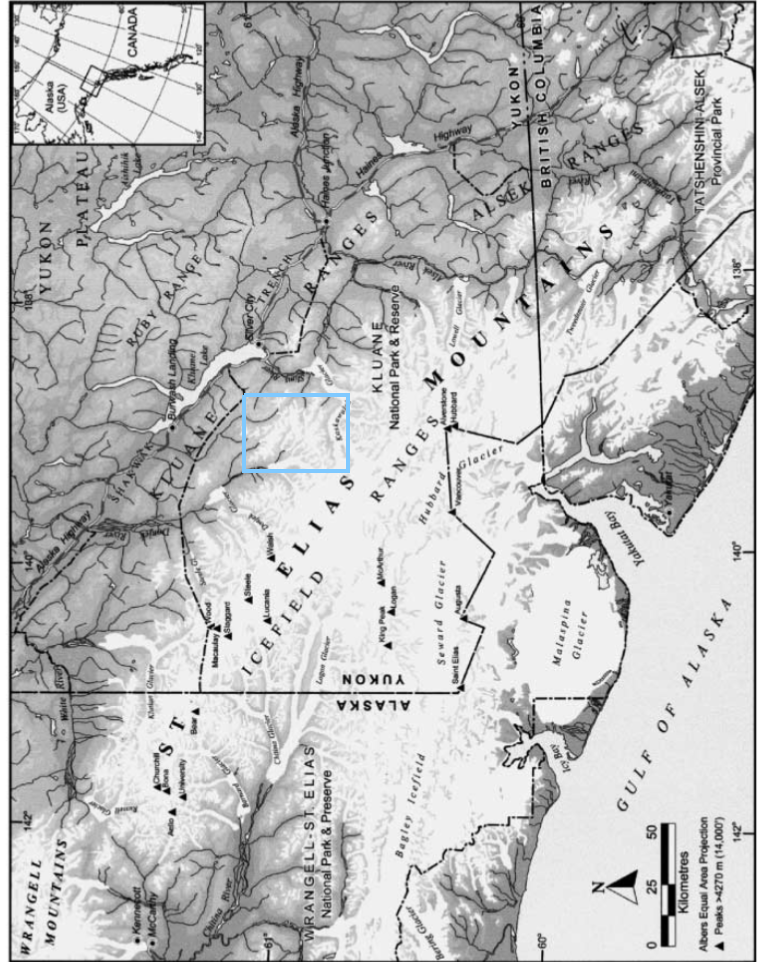
\includegraphics[width=\textwidth]{stelias.png}
  \caption{Map of the St. Elias Mountains and surrounding area. Figure taken from \cite{Danby2003}.}
        \label{map}
\end{figure}

Snow data are generally sparse in mountain regions, especially those that are isolated from humans \citep{Marcus1970}. The St. Elias Mountains (Figure \ref{map}) are one such area. These mountains contain the largest non-polar ice field and the longest valley glaciers outside of Greenland and Antarctica \citep{Marcus1970, Danby2003}. Steep climatic gradients across the mountains create sharp changes in glacier cover and mass balance \citep{Clarke2002}. This region currently has the most negative mass budget and is the largest contributor to sea-level rise in the world \citep{Kaser2006, Gardner2013}. Understanding how local glacier mass balance is affected by distribution of snow is therefore critical for accurate predictions of glacier response to a warming climate. 

Research on snow distribution and glacier mass balance in the St. Elias is limited. The first significant investigations took place under Project Snow Cornice \citep{Wood1948}. Researchers looked at snow accumulation and ice formation as well as ice-mass thermal regime, density, and depth. Studies were conducted primarily on large glaciers such as the Kaskawalsh and Seward, and thus provided insights into large-scale accumulation patterns. This initiative was then followed by the Icefield Ranges Research Project (IRRP), which was established in 1961 \citep{Danby2003}. A number of subsequent long-term studies have been established in the St. Elias since IRRP \citep[e.g.][]{Clarke1984, Paoli2009}. \cite{Wheler2014} determined the end-of-winter accumulation for the mass balance of a small alpine glacier in the Donjek Range. The study measured snow depth at a number of fixed stakes and used a multiple linear regression model --- that accounted for slope, curvature, and elevation --- to extrapolate these points and estimate basin-wide SWE. \cite{Arendt2008} also briefly studied the mass balance of a number of glaciers in the St. Elias.

Two ice cores have been retrieved from the St. Elias Mountains. The first one was taken from the summit of Mt. Logan (5340 m) in 1980 and was 103 m long. The accumulation history in this core has been used to study the local \citep{Holdsworth1991} and regional \citep{Moore2002} climate history. A second core, called the Eclipse core, was taken from a site 45 km northeast of Mt. Logan, 2 km lower in altitude, with an accumulation almost five times as large \citep{Wake2002}. This core is 160 m and has also been used for studying local and regional climate history \citep{Wake2002}. 

The weather in the St. Elias varies considerably over the range. The west side of the mountains is characterized by a cool, Marine West Coast climate due to the influence of the Pacific ocean, while the eastern side (just 250 from the ocean) is considered subarctic \citep{Marcus1970}. \cite{Taylor1969} studied the relationship between synoptic weather conditions and basin weather conditions across the St. Elias. It was observed that the mountains are oriented perpendicular to frequent and intense storms that originate in the ocean, which resultes in considerable interaction between weather and topography. When weather moves from the Gulf of Alaska, it is orographically lifted, which creates significant precipitation. If the front is perpendicular to the mountains, it can be deflected north or south, depending on the upper atmospheric flow. Fronts that are more or less aligned parallel to the mountains or very strong perpendicular fronts travel without deflection. The fronts can also stall on the west side of the mountains. Eventually, the fronts spill over the mountain divide (located to the west of the Kaskawalsh Glacier) and descend along the eastern side, which often results in decreased precipitation. This rain shadow is likely the major cause of the significant difference in accumulation and equilibrium line altitude (ELA) between the two sides of the mountains --- the marine side has an ELA of $\sim$1100 m and the continental side has an ELA of $\sim$2100 m, while at the same elevation there is three times more accumulation on the marine side \citep{Marcus1970}.

Although the characterization of synoptic conditions by \cite{Taylor1969} is useful, it was conducted during the summer when weather conditions are considerably different than during winter. \cite{Taylor1969} does note though that the weather patterns observed would likely be strengthened during winter because many of the spatial gradients are enhanced. The synoptic air masses present during the winter produce a strong temperature and moisture gradient, with warm, moisture-laden air coming from the Pacific Ocean and cold, dry air coming from the Mackenzie basin. These gradients would likely result in even more precipitation and stronger winds. The presence of a high pressure Arctic system could decrease the ability of low-pressure systems to pass over the divide, leading to a further enhancement of precipitation on the western side of the mountains. 

The study done by \cite{Taylor1969} also found weather effects on multiple scales. Synoptic conditions, including front movement, affected regional scale differences in weather and precipitation patterns. Watershed scale topography was responsible for differences in weather for nearby basins and affected wind speed and direction most significantly, while point scale topography had strong effects on snow accumulation. Orographic effects were found to be significant on all scales. 

A study done by \cite{Pomeroy1999} looked at snow mass balance in a non-glacierized alpine basin within the St. Elias. It was found that wind had a significant impact on the distribution of snow --- up to 79$\%$ of the snow was redistributed from alpine areas to (primarily) hillsides, where accumulation was tripled. In the study basin, measured accumulation ranged from 54$\%$ to 419$\%$ of the actual snowfall. However, in a subsequent study year, which had two large wet snow events, the redistribution of snow was minimal and accumulation variability was much lower. The type of snow and how susceptible it is to wind effects therefore also plays a critical role in distribution. Additionally, areas within the basin can have different accumulation patterns throughout the winter. One area within the basin studied by \cite{Pomeroy1999} had almost no redistribution (despite heavy winds) from the beginning of winter through to March. After this, all of the snow was lost even though additional accumulation events occurred in the basin. This could indicate a dependence of redistribution on weather conditions such as temperature, or that a critical depth was reached that allowed for redistribution to occur. Sublimation was also observed in the basin, but the amount of snow lost through this process could not be determined. Yet given that sublimation occurs several orders of magnitude faster when blowing snow is present and approximately 20$\%$ of winter days were observed to have blowing snow, it could have a significant impact.

There is clearly a strong need for a more comprehensive understanding of snow accumulation in the St. Elias Mountains. Although a few studies have examined accumulation, no studies have examined the distribution of snow and how it varies spatially. This is especially true of small alpine glaciers in the St. Elias Mountains, since most of the accumulation differences have been observed on large glaciers. It is likely that orographic lifting as well as wind redistribution and preferential deposition play major roles in determining accumulation on small alpine glaciers, so future studies should focus on the impact of these factors. 

\chapter{Proposed research}%%%%%%%%%%%%%%%%%%%%%%%%%%%

 \begin{figure*}
           \includegraphics[height=19cm]{SnowSpatialVariability.png}
       \caption{Visual representation of proposed research}
       \label{flowchart}
\end{figure*}

The proposed research aims to examine the spatial and temporal variability of snow distribution in the St. Elias Mountains using direct measurements and statistical models (Figure \ref{flowchart}). The spatial variability will be measured by conducting an extensive snow survey in May 2016. Accumulation will be measured using a combination of probing, firn coring, and snow pits on three alpine glaciers in the Donjek Range, located in the eastern part of the St. Elias Mountains. A combination of statistical techniques, including basic statistics, variograms, and regressions, will then be used to investigate spatial variability at multiple scales. Weather-typing will also be used to examine meso-scale weather conditions that affect precipitation distribution. 

The three glaciers chosen for this study can be seen in Figure \ref{donjek}. Glaciers in the Donjek Range are unnamed but working names have been employed by \cite{Crompton2016} and are adopted for this work. Glacier 4, Glacier 2, and Glacier 12 were selected. These glaciers were chosen because they are safe to travel on (with most of the glacier accessible on skis), have SPOT5 DEM coverage (highest resolution), and are a small enough (see Table \ref{glacierstats}) to allow for reasonable coverage using point measurement can be obtained. The selected glaciers also have similar orientations and one central glacier-filled valley (similar shape). Additionally, these glaciers are spread throughout the Donjek Range and are located increasingly further from the large-scale topographic divide (located at the head of the Kaskawalsh Glacier \citep{Taylor1969}) allowing for the potential investigation of distance from mountain divide as an effect on regional snow distribution. The three glaciers are also located on different sides of the range-scale topographic divides, which run roughly from west to east in the southern area and from south to north in the eastern area and form an `L' shape. Glacier 4 is located on the southern side of the first arm, Glacier 2 is located on the northern side of the first arm and the western side of the second arm, and Glacier 12 is located on the eastern side of the second arm. From anecdotal observations, these different configurations likely affect the winter balance of glaciers in the Donjek Range with glaciers on the southern side of the first arm receiving more snow.

\begin{figure}
  \begin{minipage}[c][22cm][t]{\textwidth}
        \vspace*{\fill}
  \centering
  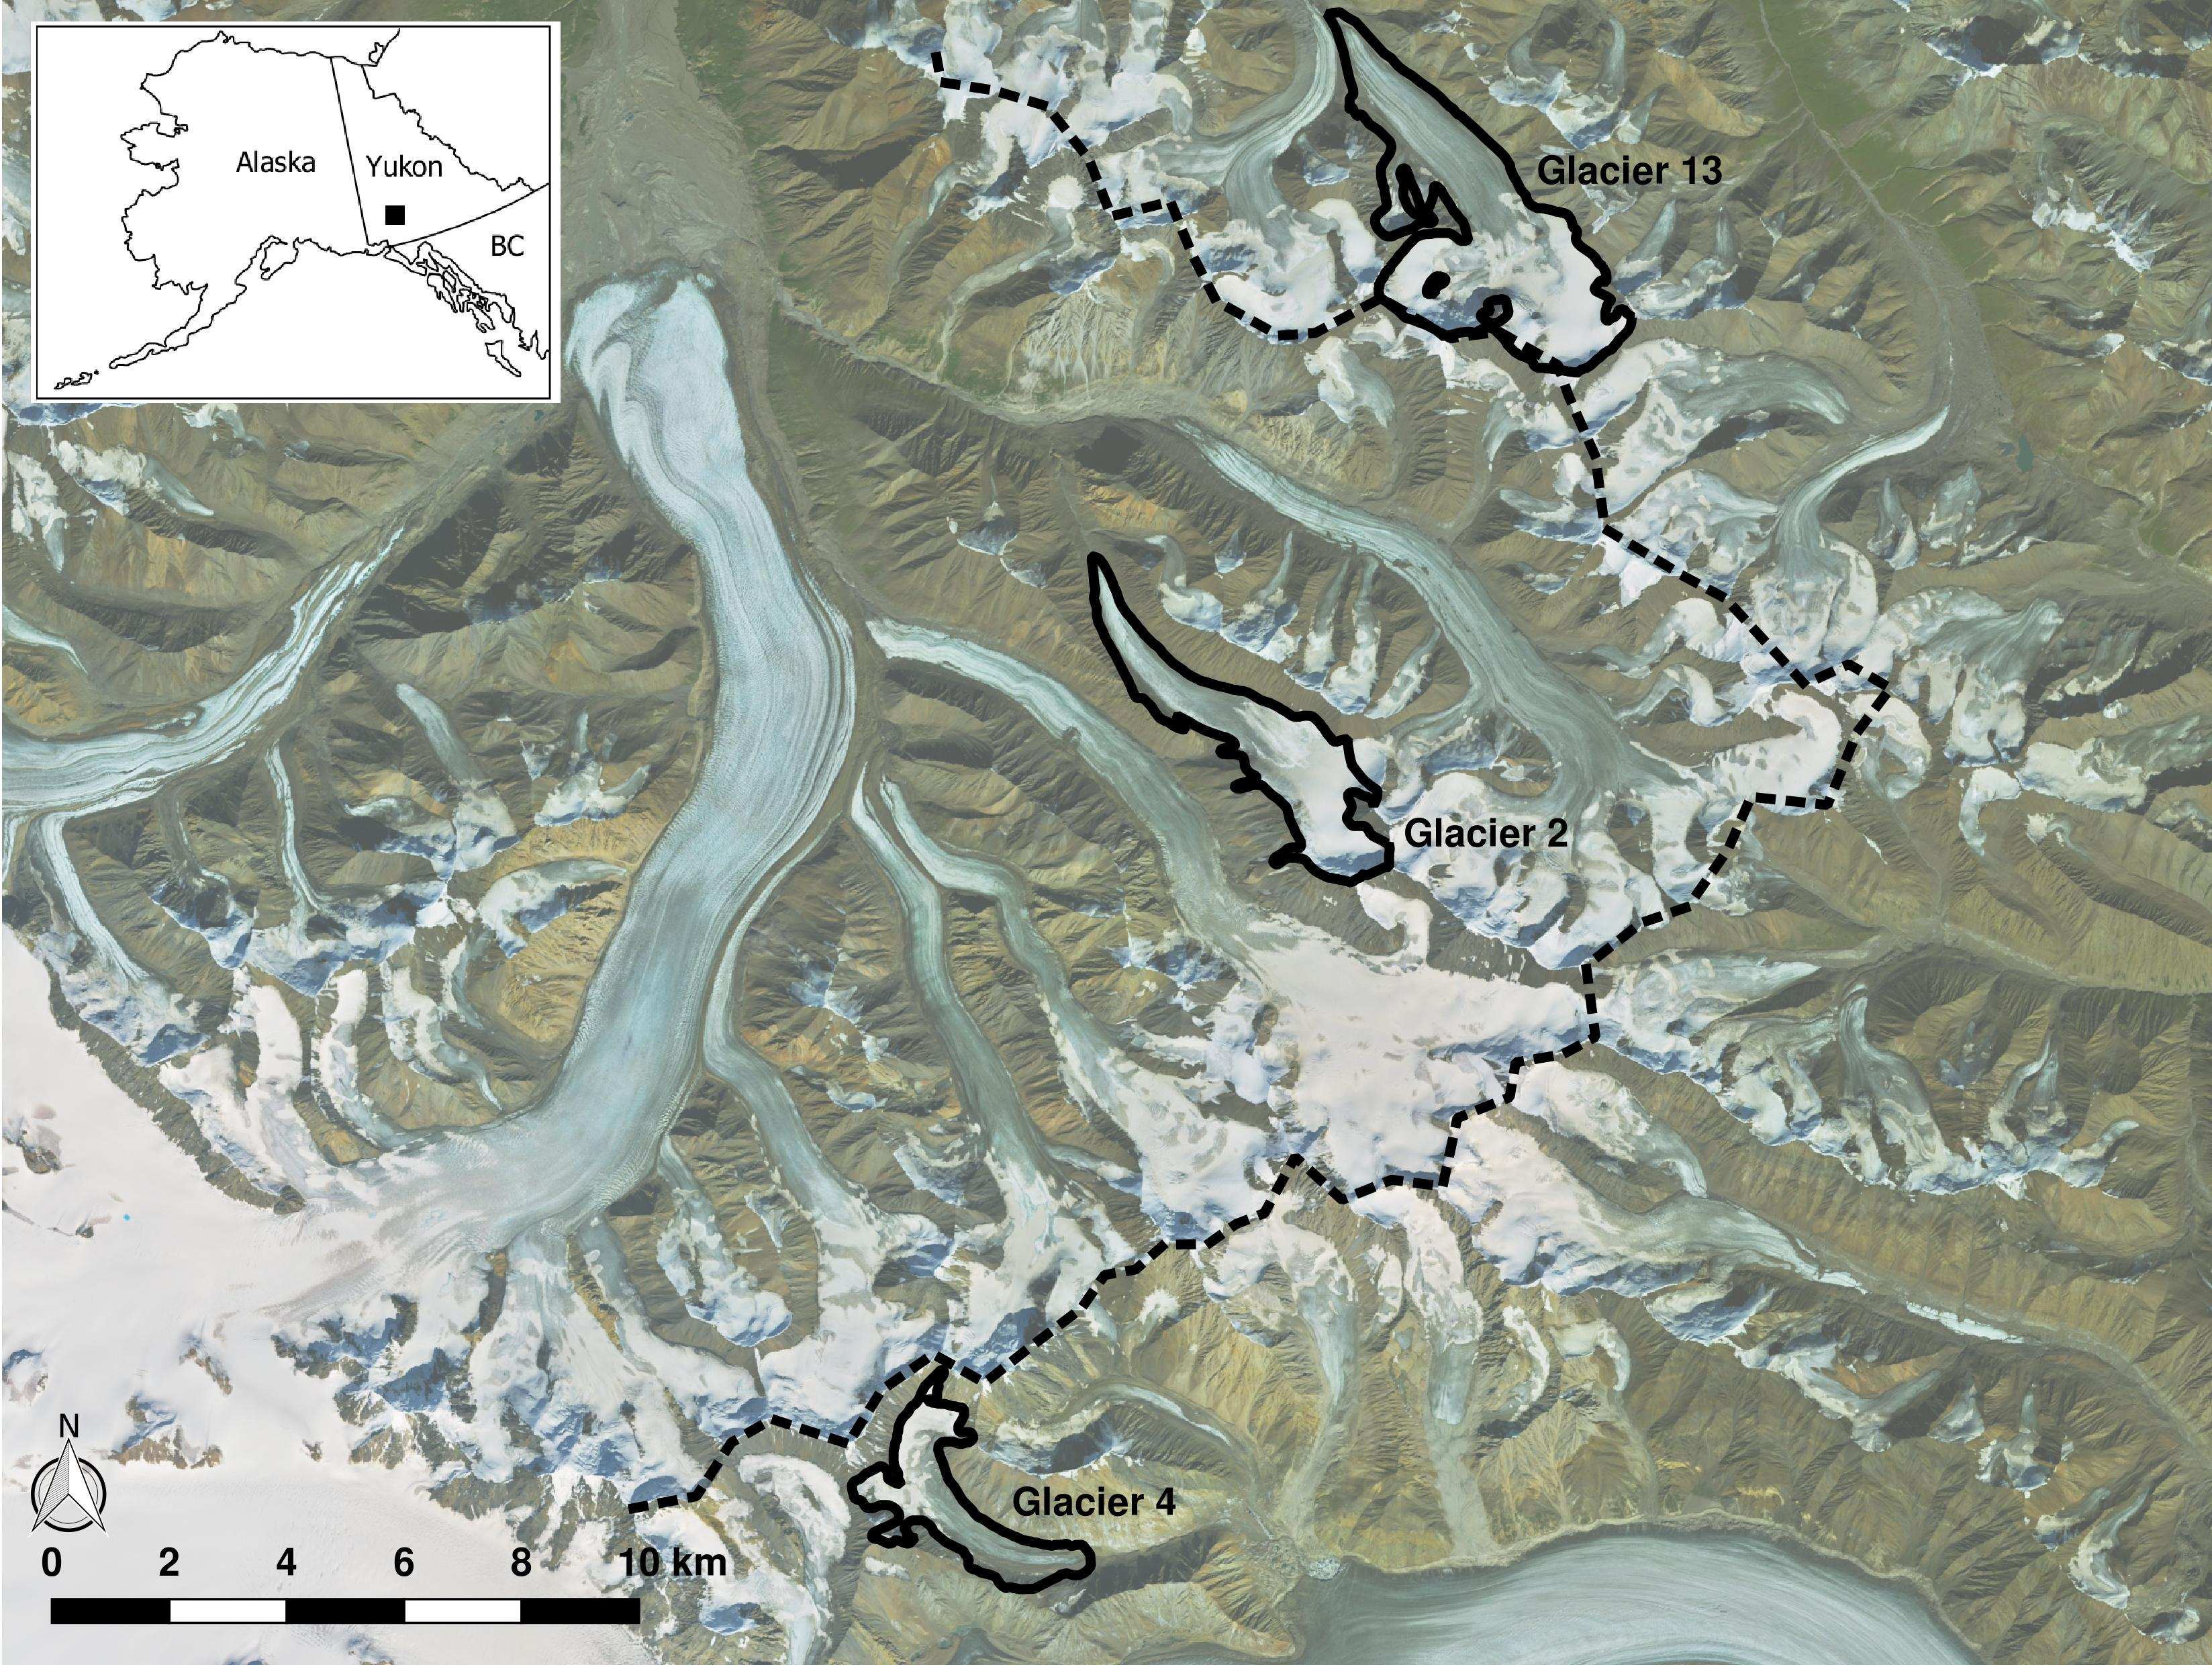
\includegraphics[height=10.5cm]{chosenglaciers.jpeg}
  \subcaption{Donjek Range with study glaciers. From left to right: Glacier 4, Glacier 2, Glacier 12. Dashed line indicates local topographic divide, which forms an `L' shape.}
  \par\vfill
  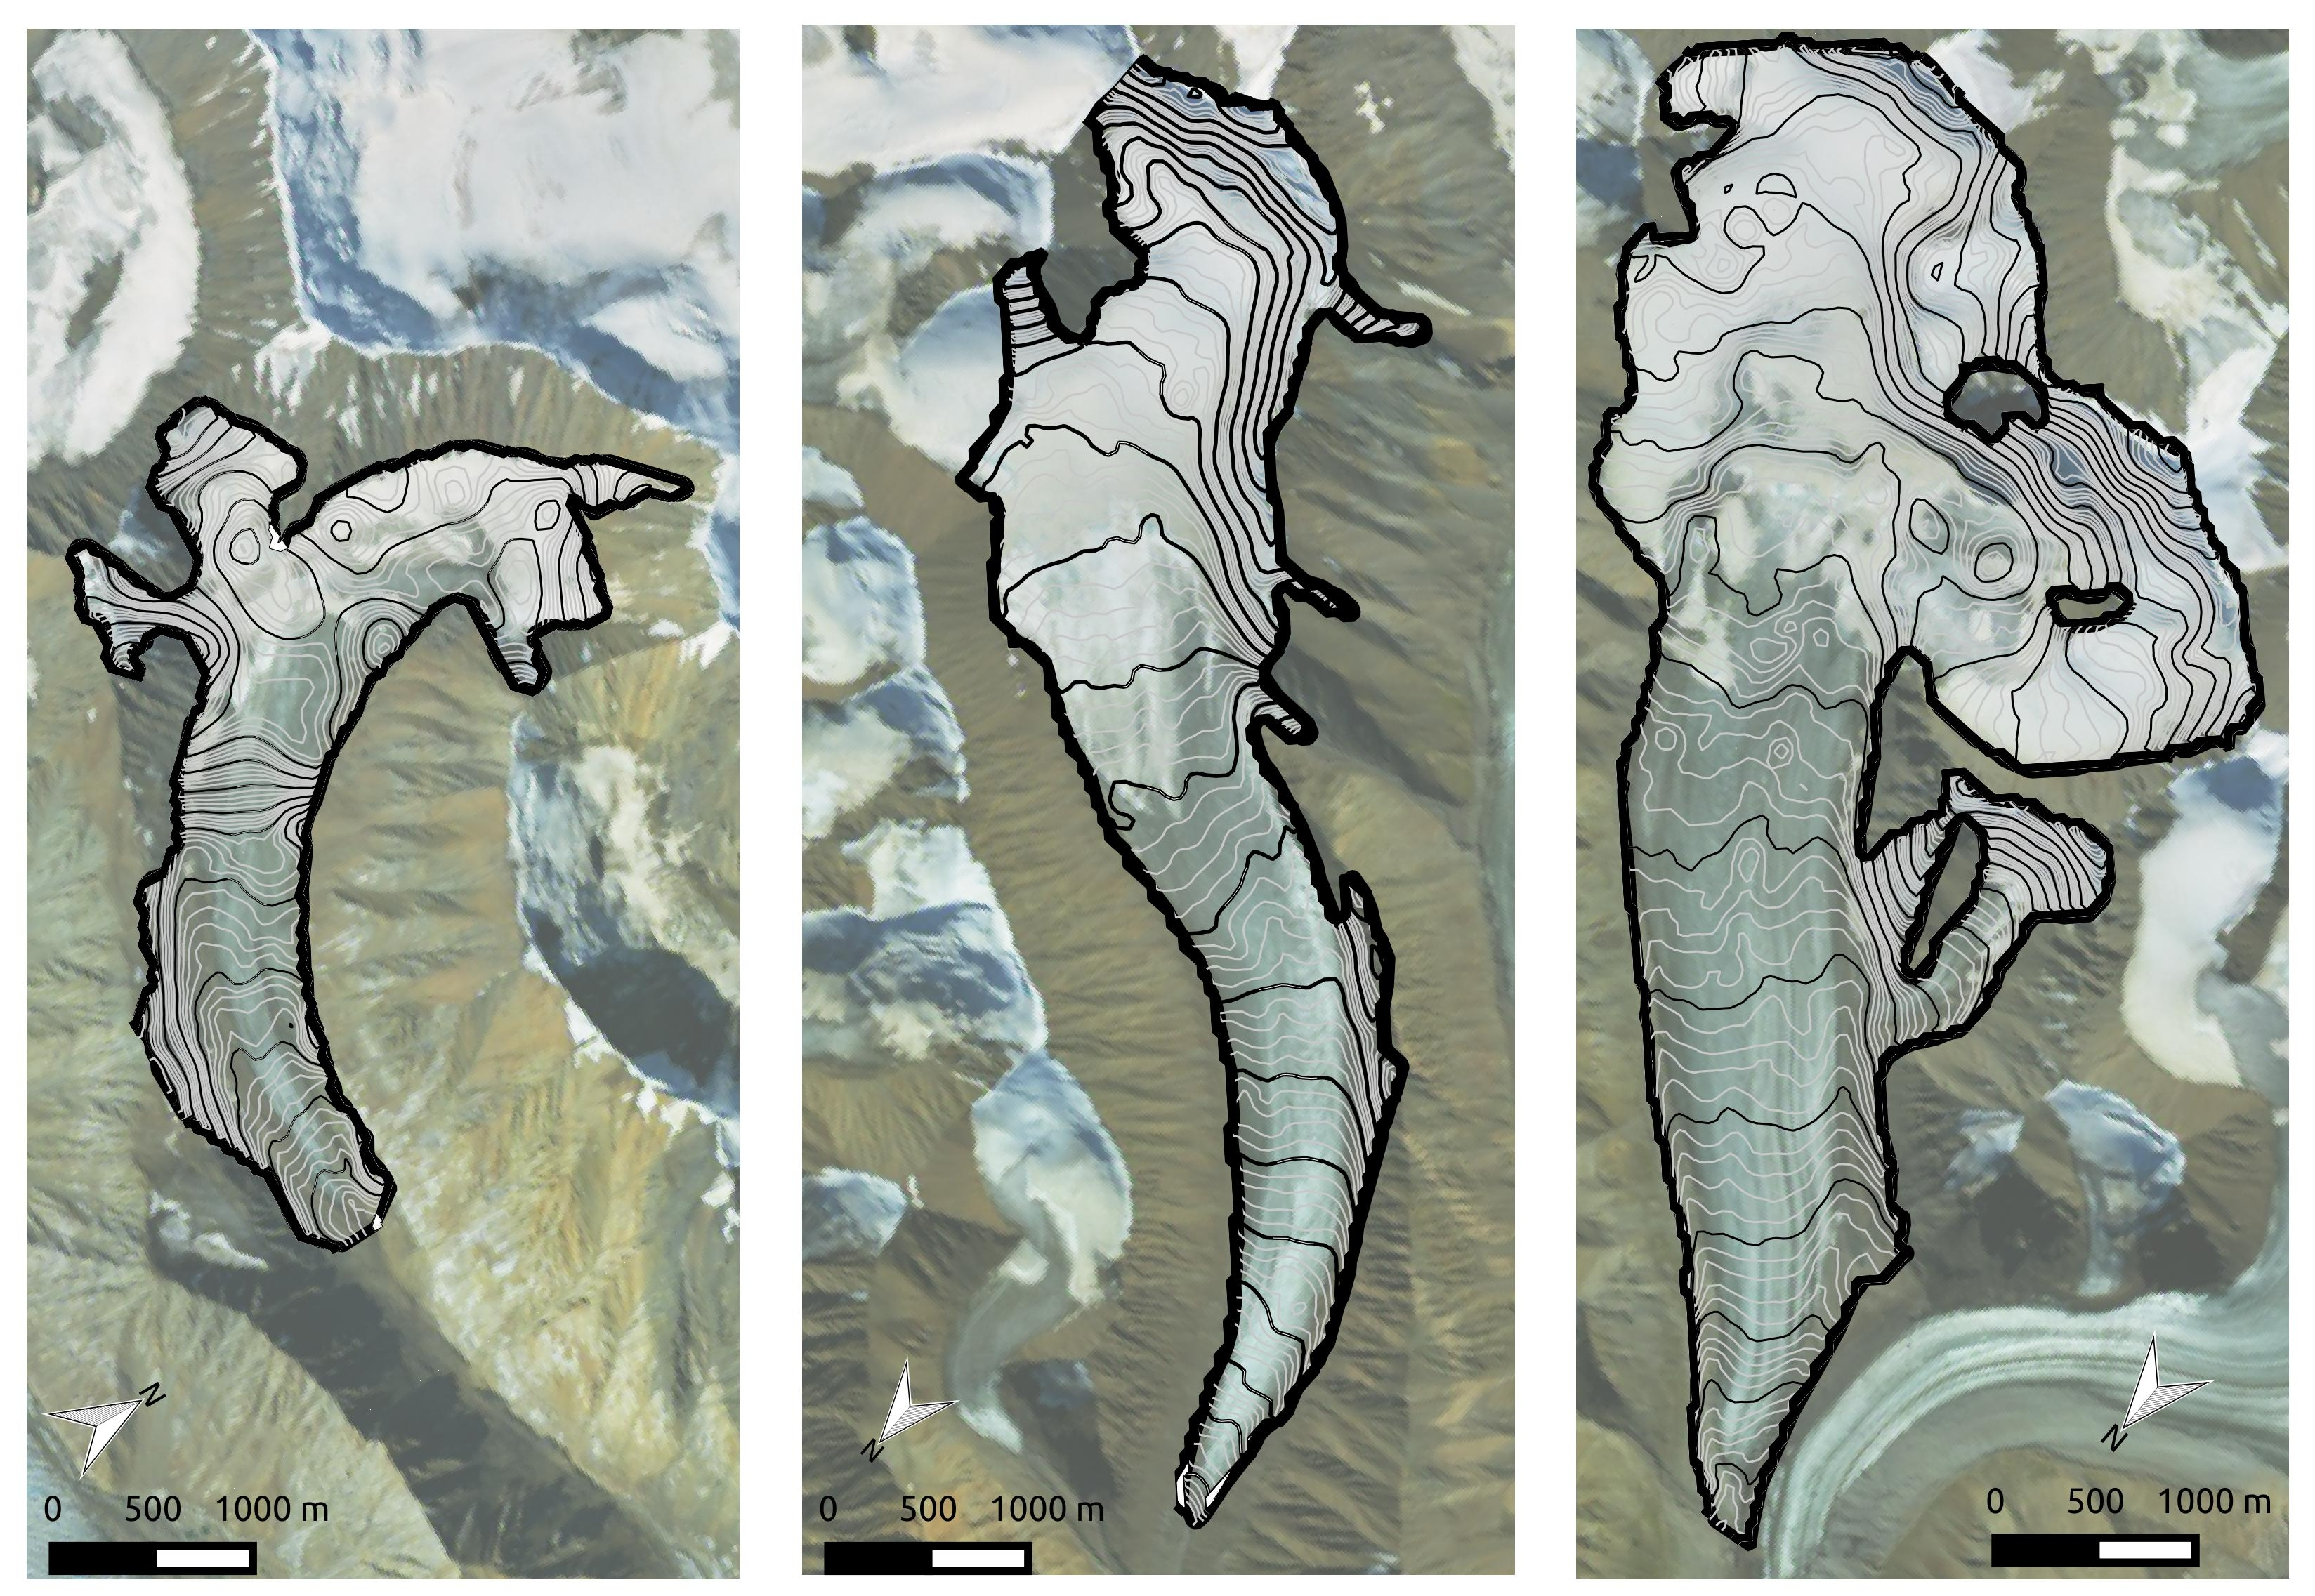
\includegraphics[height=9.5cm]{threeglaciers.jpeg}
  \subcaption{Study glaciers with 50 m contour lines. From left to right: Glacier 4, Glacier 2, Glacier 12.}
\end{minipage}%
\caption{Study glaciers in the Donjek Range.}
\label{donjek}
\end{figure}

\section{Snow Measurement} 

Each glacier was divided into seven regions to determine sampling schemes and their locations. This allowed for snow depth and density be taken throughout a large portion of the glacier area. The glaciers were divided into three attitudinally distributed areas, with the upper area encompassing the accumulation zone, the middle area encompassing the upper half of the ablation zone, and the lower area encompassing the lower half of the ablation zone. During the snow survey, approximately one day will be spent taking measurements in each area. With these divisions, the ablation area will have a higher density of snow probe, firn core, and snow pit measurements than the accumulation area. Since measurements are more difficult and time consuming to make in the accumulation area, measurement efforts will be focused on the ablation area, where the snow pack is well defined. Higher density sampling in the ablation zone may also be warranted because \cite{McGrath2015} found that the highest variability in SWE was in the ablation zone, especially in sections that had rough and crevassed ice.

The middle and lower areas were further divided into left, central, and right areas. The left and right areas encompass the margin of the glacier and were defined as being within 300 m of the ice edge (as mapped by the Randolph Glacier Inventory (RGI 5.0) \citep{Pfeffer2014}), while the central area encompasses the central part of the glacier between the margins. This division was chosen because the snow distribution is likely to be affected by different processes at the margins compared to the centre. The margins are closer to steep rock slopes, which can affect the wind patterns and radiation at the snow surface. Avalanching can also affect snow distribution along the margins \citep{Bloschl1991}. 

\begin{table}[t!]
\centering
\caption{Area, length, and elevation descriptors of three chosen glacier.}
\label{glacierstats}
\begin{tabular}{|l|c|c|ccc|}
\hline
\multicolumn{1}{|c|}{} & \multirow{2}{*}{\textbf{Area (km$^2$)}} & \multirow{2}{*}{\textbf{Length (km)}} & \multicolumn{3}{c|}{\textbf{Elevation (m)}}         \\
\multicolumn{1}{|c|}{} &                                         &                                       & \textbf{Minimum} & \textbf{Maximum} & \textbf{Mean} \\ \hline
Glacier 4              & 5.26                                    & 6.2                                   & 1573             & 2854             & 2321          \\
Glacier 2              & 6.91                                    & 7.4                                   & 1906             & 3098             & 2472          \\
Glacier 12             & 25.59                                   & 9.5                                   & 1775             & 3037             & 2434          \\ \hline
\end{tabular}
\end{table} 

Probing will be done at point, hillslope, and watershed scales on the three glaciers (regional scale) in a number of patterns and orientations in an attempt to estimate snow distribution at multiple scales (Figure \ref{sampling}). For the point scale, the star design will be used to measure snow depth within 40x40 m grids (SPOT5 DEM resolution). For the hillslope scale, the hourglass with inscribed circle (referred to just as hourglass) will be used to measure snow depth within an entire elevation band of the glacier, with the upper and lower transects also serving as transverse transects. Cross transects will be completed opportunistically when areas of high curvature are present. A centreline profile and additional transverse transects will also be probed, which can be combined with hourglass measurements to estimate watershed-scale mass balance. A comparison of these measurements between the three study glaciers will allow for investigation of regional scale variability. Sampling schemes will be placed to ensure that SWE is measured in locations that represent a full range of topographic parameters found on each glacier. 

For each glacier, the following series of snow depth measurements have been planned:
\begin{itemize}
\item Star design in a random location in thirteen regions of the ablation zone, with seven in the lower ablation area and six in the upper ablation zone (125 points each, random distance between 0.1 m and 1.5 m)
\item Hourglass in two regions of the glacier ablation zone and span the entire width (random distance between 5 and 20 m). The upper and lower portions will thus also serve as cross-glacier transects.
\item Transverse transects in three locations: one close to the terminus and two between the hourglass schemes (random distance between 5 and 20 m).
\item A centre-line transect with a low resolution ($\sim$100m). 
\end{itemize}

 \begin{figure*}
           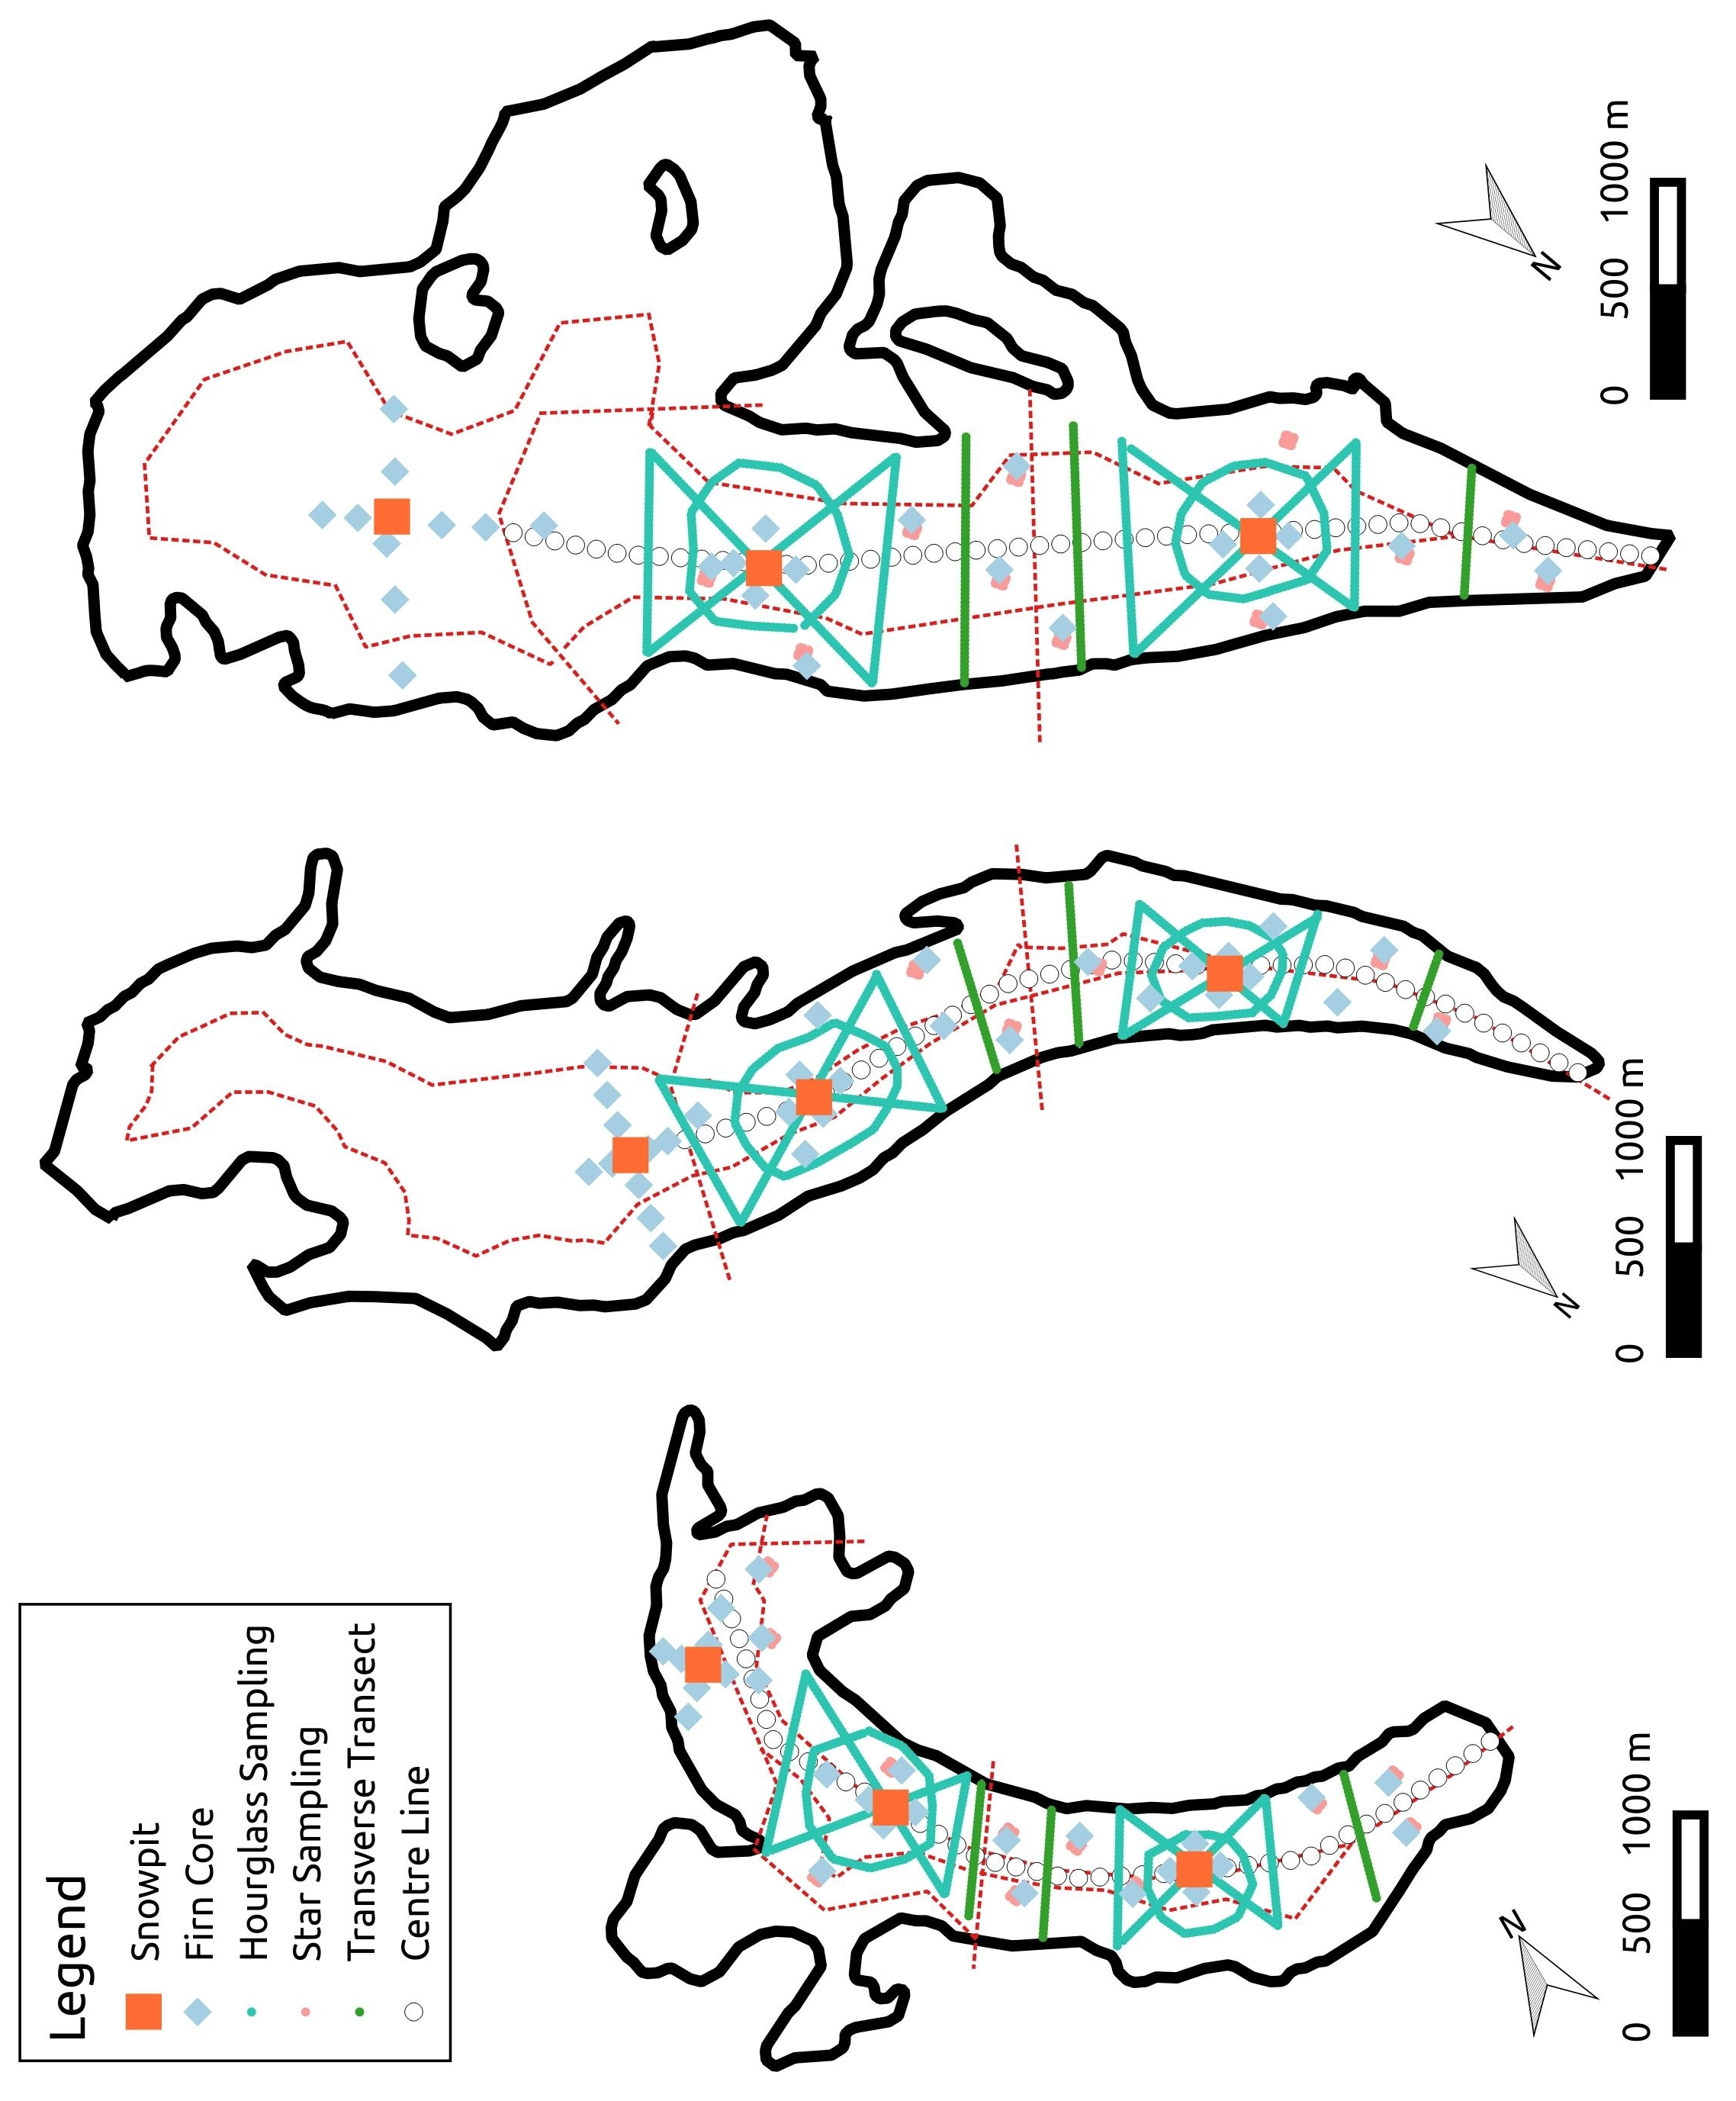
\includegraphics[height=19cm]{SamplingDesign.jpeg}
       \caption{Planned sampling design on Glaciers 4, 2 and 12.}
       \label{sampling}
\end{figure*}

Snow density will be measured in various areas of each glacier. A firn corer will be used to determine bulk density of the snow column by extracting snow cores (known volume) and weighting them. This instrument will be used because it allows for faster estimation of snow column density than snow-pit derived density. The measurements obtained with the firn corer will be compared to density measured in a snow pit using a wedge cutter, which is considered the most accurate way to measure density but is more time consuming \citep{Ostrem1991}. In areas with shallow snow packs, a Federal sampler (i.e. SWE tube) will be used for snow density measurements. Other snow properties observed in the snow pit, including stratigraphy and snow pack temperature will also be recorded.

For each glacier, the following series of snow density measurements have been planned (note that each measurement also serves as a depth measurement):
\begin{itemize}
\item Firn core at the edge of each star design located throughout the glacier.
\item Four firn cores at the centre of each hourglass scheme.
\item Approximately six firn cores in the transverse direction and four in the along-flow direction of the accumulation area.
\item Snow pit measurements at the centre of each hourglass schemes and one in the accumulation aree (allows for comparison of firn core and snow-pit density)
\end{itemize}

\section{Statistical Analysis}

Spatial variability of snow accumulation at multiple scales will be investigated using a number of statistical techniques. Variograms will be constructed from all snow-depth measurements within a basin. This will allow for an investigation of relevant length scales and scale breaks that may address the autocorrelation of snow depth on glaciers and identify how much variance can be observed using our methods (variogram nugget). Identification of scale breaks could also help determine processes that drive snow distribution patterns at various scales. 

At the point scale, the goal is to determine measurement error. To accomplish this, variability of snow depth within a grid cell will be quantified using basic statistical descriptors (e.g. standard deviation) of measurements from the star sampling schemes. It is valuable to estimate the uncertainty of a snow depth measurement at the resolution of the DEM used. 

Regressions of SWE and DEM-derived terrain parameters will be done to investigate variability at the hillslope scale. Terrain parameters, including elevation, slope, curvature, ``northness'', aspect, and wind exposure/shelter, will be calculated from SPOT5 DEMs (40 x 40 m resolution). Both linear statistical methods (e.g. multiple linear regression) and non-linear methods (e.g. regression tree models) will be applied to best try to capture the relationships between geography and accumulation. The regression method that is able to capture the most variance will be used to interpolate between accumulation measurements to obtain a spatial distribution of SWE. 

Variability at the watershed scale will be investigated by comparing winter balance estimates using different combinations of observed snow distribution and terrain parameters used for the regression. Different subsets of measured SWE values will be used to determine regressions and estimate winter balance, which will provide a range of possible winter-balance values. Comparing interpolated values of SWE from various regressions with measured values will examine the error when interpolating between point observations. This analysis is likely to provide insight into optimizing future glacier snow surveys.

At the regional scale, various analyses will be conducted. First, the transferability of regressions will be investigated by applying the regressions from one glacier to the other two and evaluating their performance. 

Second, an investigation into the mesoscale weather conditions in the Pacific northwest during the 2015--2016 winter season will be done in an attempt to explain regional scale differences in accumulation. Weather conditions, including geopotential height, integrated vapour transport (IVT), and mean sea-level pressure, in the North Pacific will be obtained from ERA-Interim reanalysis data and statistical methods, including PCA and neural networks, will then be applied to find weather patterns. The frequency and types of patterns observed at the mesoscale, such as atmospheric rivers of IVT \citep{Neiman2008, Roberge2009}, could provide insight into moisture sources for the Donjek Range and how they affect glaciers at different distances from the large-scale topographic divide as well as various orientations to range-scale topographic divides. 

Links with other studies that examined relationships between local precipitation and mesoscale and synoptic weather conditions will aid in understanding processes that affect regional snow distribution differences and in formulating hypotheses for future research. For example, \cite{Serreze1995} and \cite{Lackmann1998} found that vapour fluxes originating in the Pacific Ocean tend to peak in the lower troposphere (800 hPa) so the presence of a high mountain range is likely to block these sources. Additionally, \cite{Neiman2008} observed that on the west coast, atmospheric rivers are responsible for twice as much precipitation as all storms and that atmospheric rivers have a tendency to increase SWE in the autumn and winter and decrease SWE in the spring. Furthermore, work done by \cite{Roberge2009} found that atmospheric rivers, which result in intense cold-season precipitation events in the Yukon, can be clustered by the general area of moisture origins and that they are associated with certain synoptic conditions in the North Pacific. A study done by \cite{Matthews2013} found that including weather type found from reanalysis data improved the simulation of daily ablation by up to 14\% compared to a temperature-index model. Although this study did not examine precipitation, it is possible that investigation of weather conditions could also improve precipitation modelling through statistical down-scaling and account for inter-annual variability in precipitation. Preliminary work to correlate synoptic patterns to glacier-wide accumulation reveals significant correlations between patterns in the 750 hPa geopotential, found using a self organizing map (SOM), and winter balance on one glacier in the Donjek Range between 2007 and 2011, which is consistent with observations made by \cite{Taylor1969} in the St. Elias Mountains. 

\section{Expected Outcomes}

The goal of this project is to improve understanding of processes and parameters that affect snow accumulation on glaciers. Currently, there is little work that addresses length scales of SWE on glaciers. A large portion of the proposed work will therefore focus on identifying length scales within glacierized basins. This will be done by constructing and analysing variograms using data from star sampling schemes as well as hourglass, transverse, and centreline sampling schemes. From this, lag distances between 0.1 m and $\sim$5 km can be plotted, which allows for identification of multiple relevant length scales. Fractal analysis could also be attempted, which may aid in the identification of scale breaks. Determining length scales is likely to provide insight into conditions and processes that affect snow distribution, including underlying topography such as crevasses as well as wind redistribution. 

Mass balance models often estimate winter balance by using interpolation methods based on only a small number of observations. It is likely that these accumulation estimates are poor representations of mass balance input. The proposed work will attempt to improve how these estimates are made by determining uncertainty in SWE measurement and interpolation, identifying topographic parameters that affect snow distribution, and examining the transferability of statistical models within a mountain range. While these aspects have been investigated in mountain environments, there are few studies that look at winter balance estimates on glaciers. By examining various statistical techniques used when calculating regressions between observed accumulation and topographic parameters (e.g. linear regression versus binary tree) as well as different methods for interpolating between measurements (e.g. kriging), a range of winter mass balance estimates can be complied. Various subsets of measured SWE can also be used in these regressions and interpolations to examine the effect of sample size and measurement location on accumulation estimates. Valuable insights into optimizing snow survey design are likely to be gained from this process. Transferability of regressions between nearby basins will also be addressed, which will aid in determining winter mass balance across mountain ranges. Examining potential impacts of mesoscale weather systems (weather typing) on mountain range snow accumulation will also contribute to improving current understanding of conditions that may affect observed snow distribution. 

There is a need for a multi-scale investigation of snow accumulation on glaciers. The proposed work aims to characterise the snow distribution by identifying relevant length scales and by investigating the uncertainty, techniques, and controlling factors associated with calculating spatial patterns of SWE. 

\section{Summary}
Snow accumulation plays a central role in alpine hydrology and has a prominent impact on glacier mass balance. In mountainous regions, accumulation is highly variable on point, hillslope, watershed, and regional scales. The contribution of accumulation to glacier mass balance is controlled mainly by the distribution of snow. Processes such as orographic lifting, preferential deposition, and wind redistribution, all arising from the interaction of atmospheric conditions and topography, strongly affect snow distribution. Statistical models have been used to relate meteorological and topographic variables to snow accumulation in order to better understand the effects of these processes. These models rely on accurate measurement of snow distribution, which can be achieved by determining SWE from snow density and depth. Results from previous studies of accumulation on glaciers have shown large spatial variability at many scales and a dependence on multiple processes that affect snow distribution. 

Accumulation in the St. Elias Mountains is poorly understood, largely because the glaciers are remote. There is a need to quantify snow accumulation in this region and how it varies both between glaciers and within glacierized basins. The proposed study would be the first within the St. Elias Mountains to examine accumulation variability at the point, hillslope, watershed, and regional scale. Well-established methods will be applied to measure accumulation variability.  These measurements will be used to investigate measurement uncertainty and relevant length scales, the role of topography in determining snow distribution, optimizing winter balance measurement, and the transferability of statistical relationship as well as regional differences in accumulation across a range. This comprehensive approach to examining spatial patterns in snow distribution on glaciers will contribute to the current understanding of processes and parameters that affect winter balance variability on glaciers. 


%%%%%%%%%%%%%%%%%%%%%%%%%%%%%%%%%%%
\chapter{Field methods and data processing}

***Still needed: close up photo of swe tube, snowpit cut outs?

%%%%
\section{Field Design}
%%%%

\subsection{Sampling Scheme and Naming System}

Three glaciers within the Donjek Range were chosen as study sites and can be seen in Figure \ref{studysites}. Glaciers in the Donjek Range are unnamed but working names have been employed by \cite{Crompton2016} and are adopted for this work. Glacier 4, Glacier 2, and Glacier 13 were selected. These glaciers were chosen because these glaciers are spread throughout the Donjek Range and are located increasingly further from the large-scale topographic divide (located at the head of the Kaskawalsh Glacier \citep{Taylor1969}). The three glaciers are also located on different sides of the range-scale topographic divides, which run roughly from west to east in the southern area and from south to north in the eastern area and form an `L' shape. Glacier 4 is located on the southern side of the first arm, Glacier 2 is located on the northern side of the first arm and the western side of the second arm, and Glacier 13 is located on the eastern side of the second arm. The selected glaciers also have similar orientations and one central glacier-filled valley (similar shape). Within the Donjek Range, these glaciers have good SPOT5 DEM coverage, which provides the highest resolution DEM available for this area. Additionally, the majority of the three glaciers is accessible on foot and the total area is small enough (see Table \ref{glacierstats}) to allow for reasonable coverage using point measurements.

The sampling scheme for each glacier was chosen to be similar so that comparison between glaciers could be done more readily. Each glacier was divided into the accumulation area, upper ablation area, and lower ablation area. In the accumulation area, a central snowpit location was chosen. Additionally, a series of approximately ten snow coring locations was chosen throughout the accumulation area. Steep sections and glacier margins were avoided. In both the upper and lower ablation area a number of linear and curvilinear transects were mapped, which included an `hourglass and circle' (Parr, C., 2016 personal communication) as well as a transverse (below the hourglass) and midline transect. The length and width of each transect was adjusted to span the full dimension of its corresponding area. Snowpit locations in the ablation area were chosen to be at the centre of each hourglass. An overview of the sampling design can be seen in Figure \ref{transect_planned}.

The full ablation area was also divided into seven zones of approximately equal elevation intervals. Three locations within each zone were then randomly selected for zigzag \citep{Shea2010} measurements (Figure \ref{zigzag_planned}) and the three locations were randomly labelled as different priorities. The goal was to complete one zigzag in each zone. If possible, the measurement would be completed at the `Priority A' location but if it was not possible due to dangerous conditions then the `Priority B' or `Priority C' locations would be chosen. This allowed for random locations to be used but with the flexibility to adjust locations in the field. SWE measurements would be taken within each zigzag, and at snowpit locations with the ablation area.  

The location of each snow depth and density measurement is imported into hand-held GPS devices (Garmin GPSMAP 64s) as a waypoint with a unique name. Points that are part of a transect have a name with the glacier number, the transect and area that the point belongs to, and a three-digit sequential number. The code for the transect area and type includes two letters. The first letter is either `A' for `accumulation area', `U' for `upper ablation area', or `L' for `lower ablation area'. The second letter indicates the transect type, with `H' for `hourglass', `T' for `transverse transect', `C' for `circle', and `M' for `midline'. For example, the name G04\_UM023 is the 23rd point on the Midline transect in the Upper ablation area of Glacier 4, and G13\_LC134 is the 134th point on the circle in the lower ablation area of Glacier 13. Other points that are not part of a transect also follow a similar naming convention. The snowpit locations use the code `SP' (e.g. G04\_LSP is the snowpit located in the lower ablation zone of Glacier 4) and the firn coring locations have the code `FC' and a two digit number (e.g. G02\_AFC04 is the fourth firn core location in the accumulation area of Glacier 2).

The zigzag points have a name with the glacier number, the zone that they were located in, the zigzag priority, and the vertex number. The zone and priority (A, B, C) are indicated by a `Z', then the zone number, and then an `A', `B', or `C'. The vertex number is indicated by a `ZZ' and then a sequential number. For example, the vertex labelled G02\_Z2C\_ZZ04 is on Glacier 2 in zone 2 and the fourth point of a priority C zigzag. The vertex labelled G13\_Z7A\_ZZ08 is on Glacier 13 in zone 7 and the eighth point of a priority A zigzag. An example of a zigzag sampling scheme can be seen in Figure \ref{zigzag_vertex}.

\begin{landscape}
\begin{figure}
	\centering
	\fbox{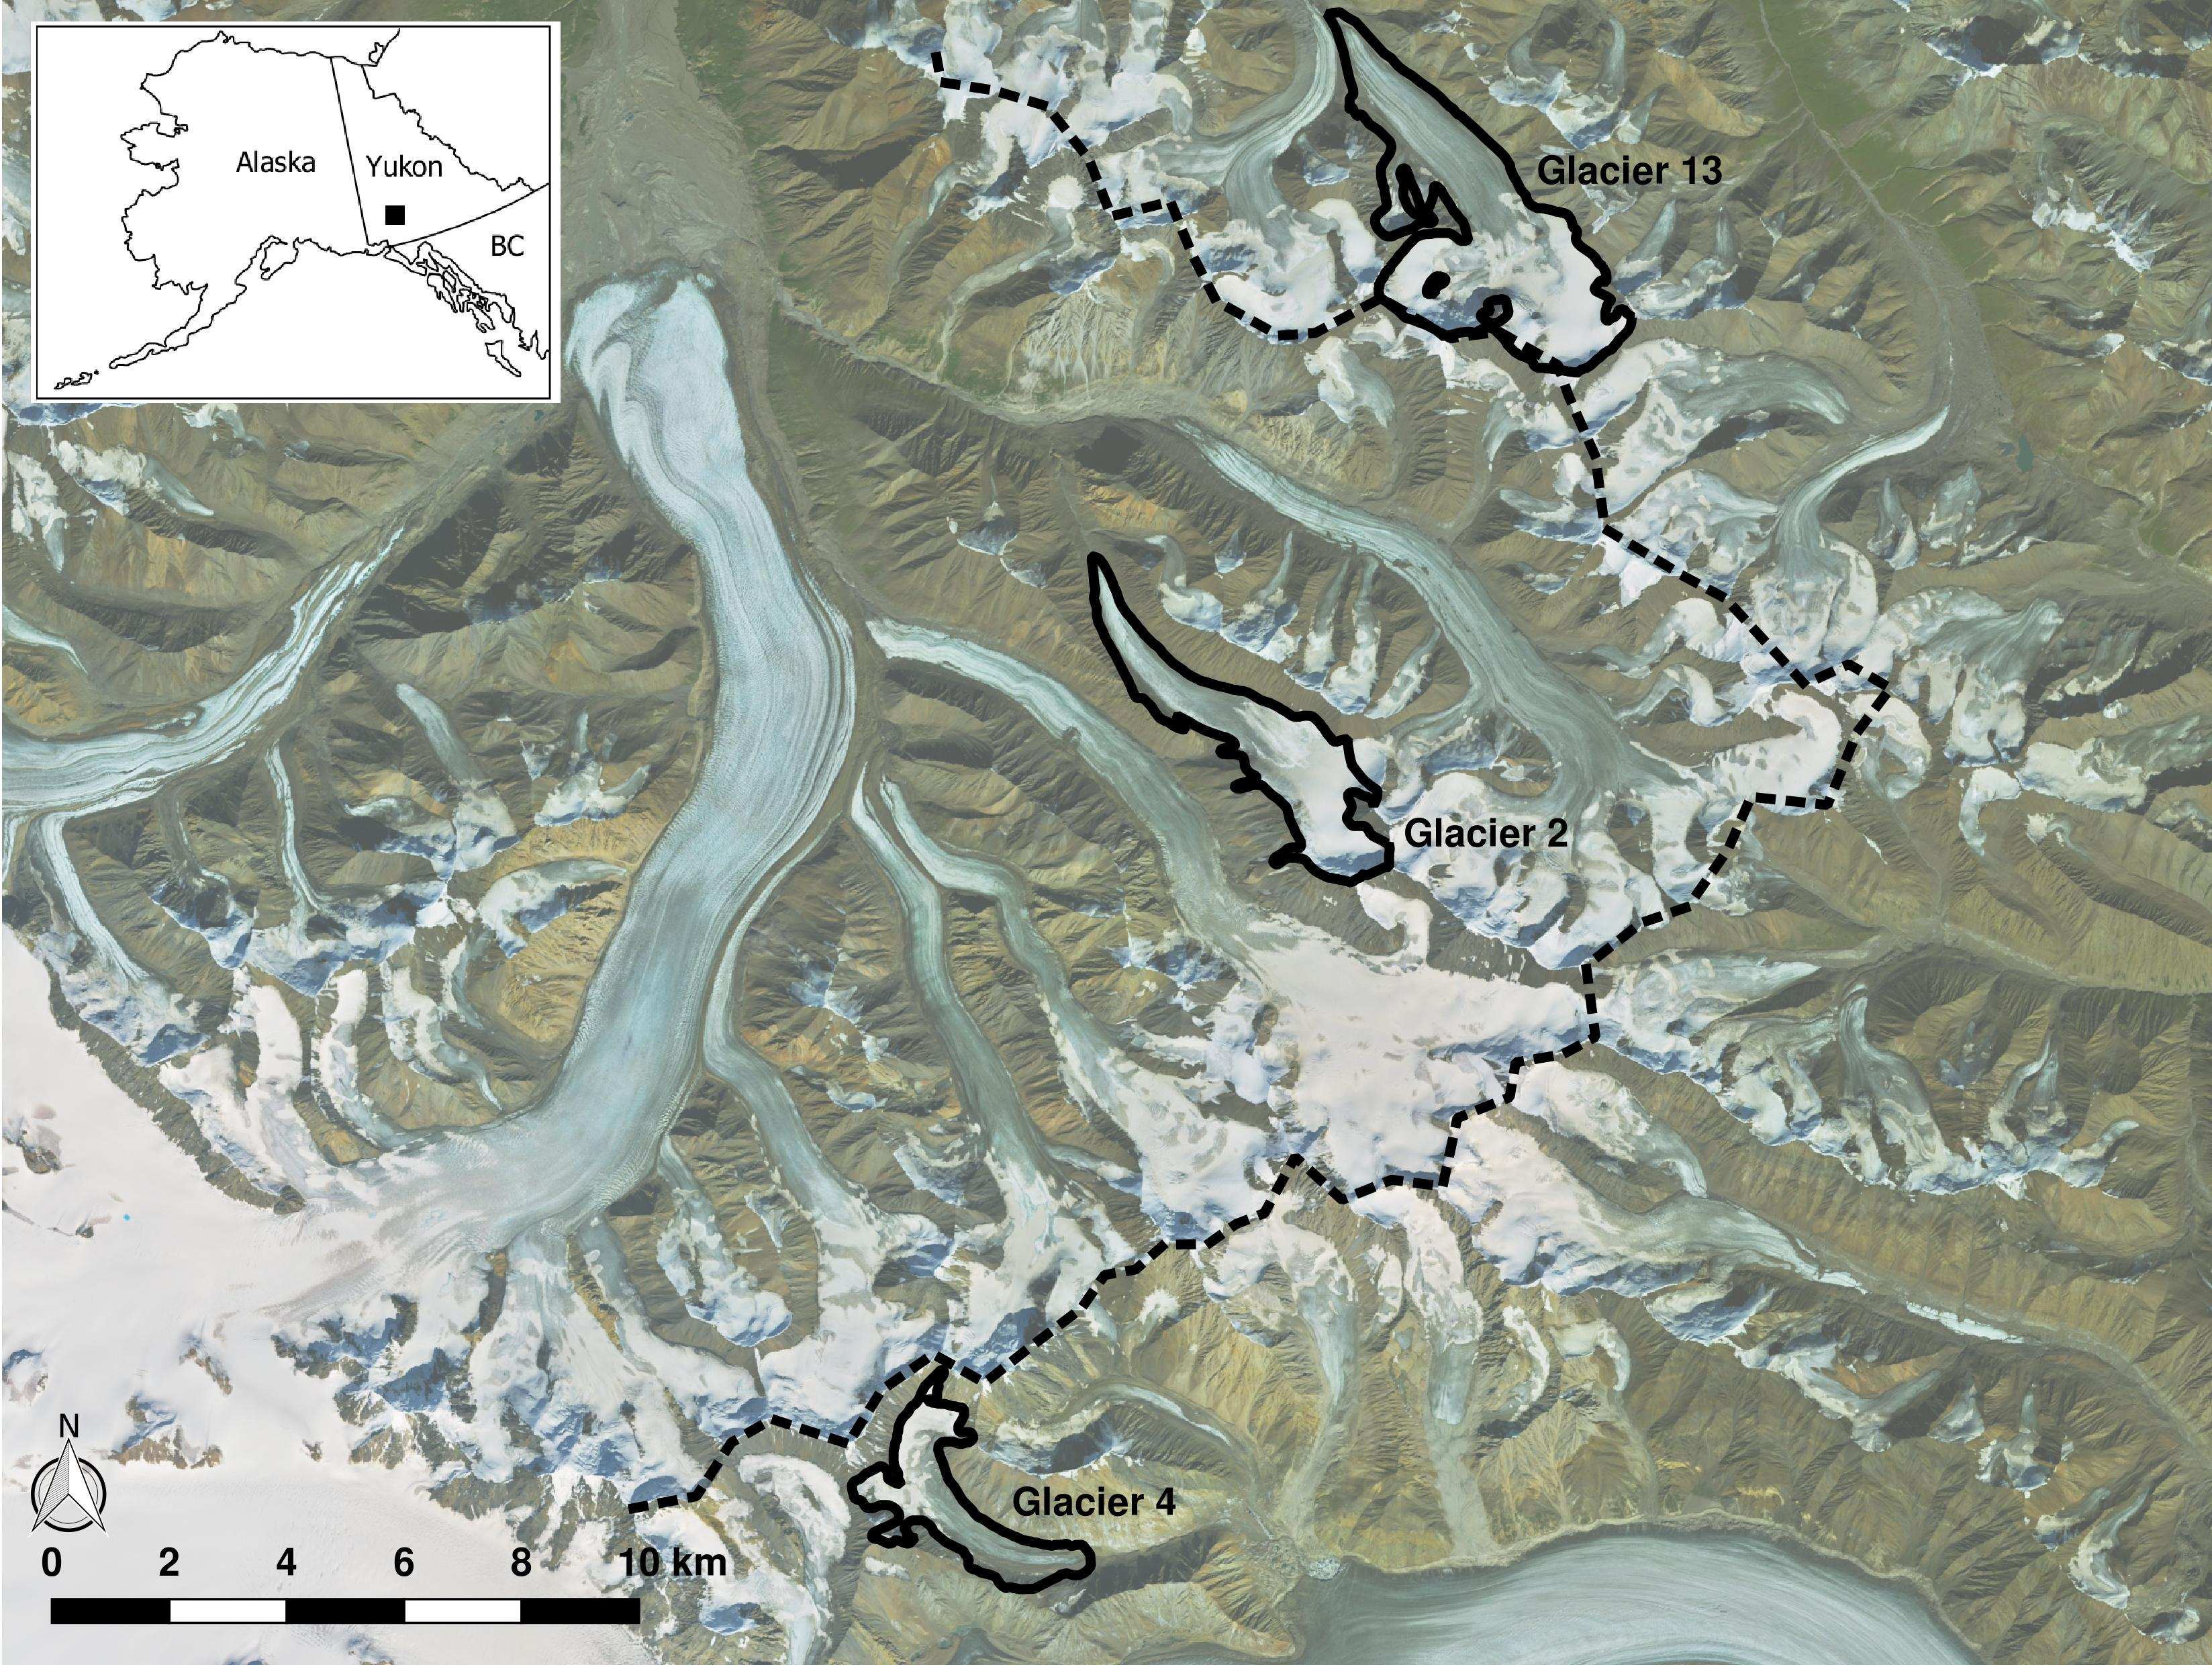
\includegraphics[height = 0.95\textwidth]{chosenglaciers.jpeg}}\\
	\caption{Study glaciers in the Donjek Range, Yukon (see inset). The topographic divide is shown as a dashed line.}
	\label{studysites}
\end{figure}

\begin{figure}
	\centering
	\fbox{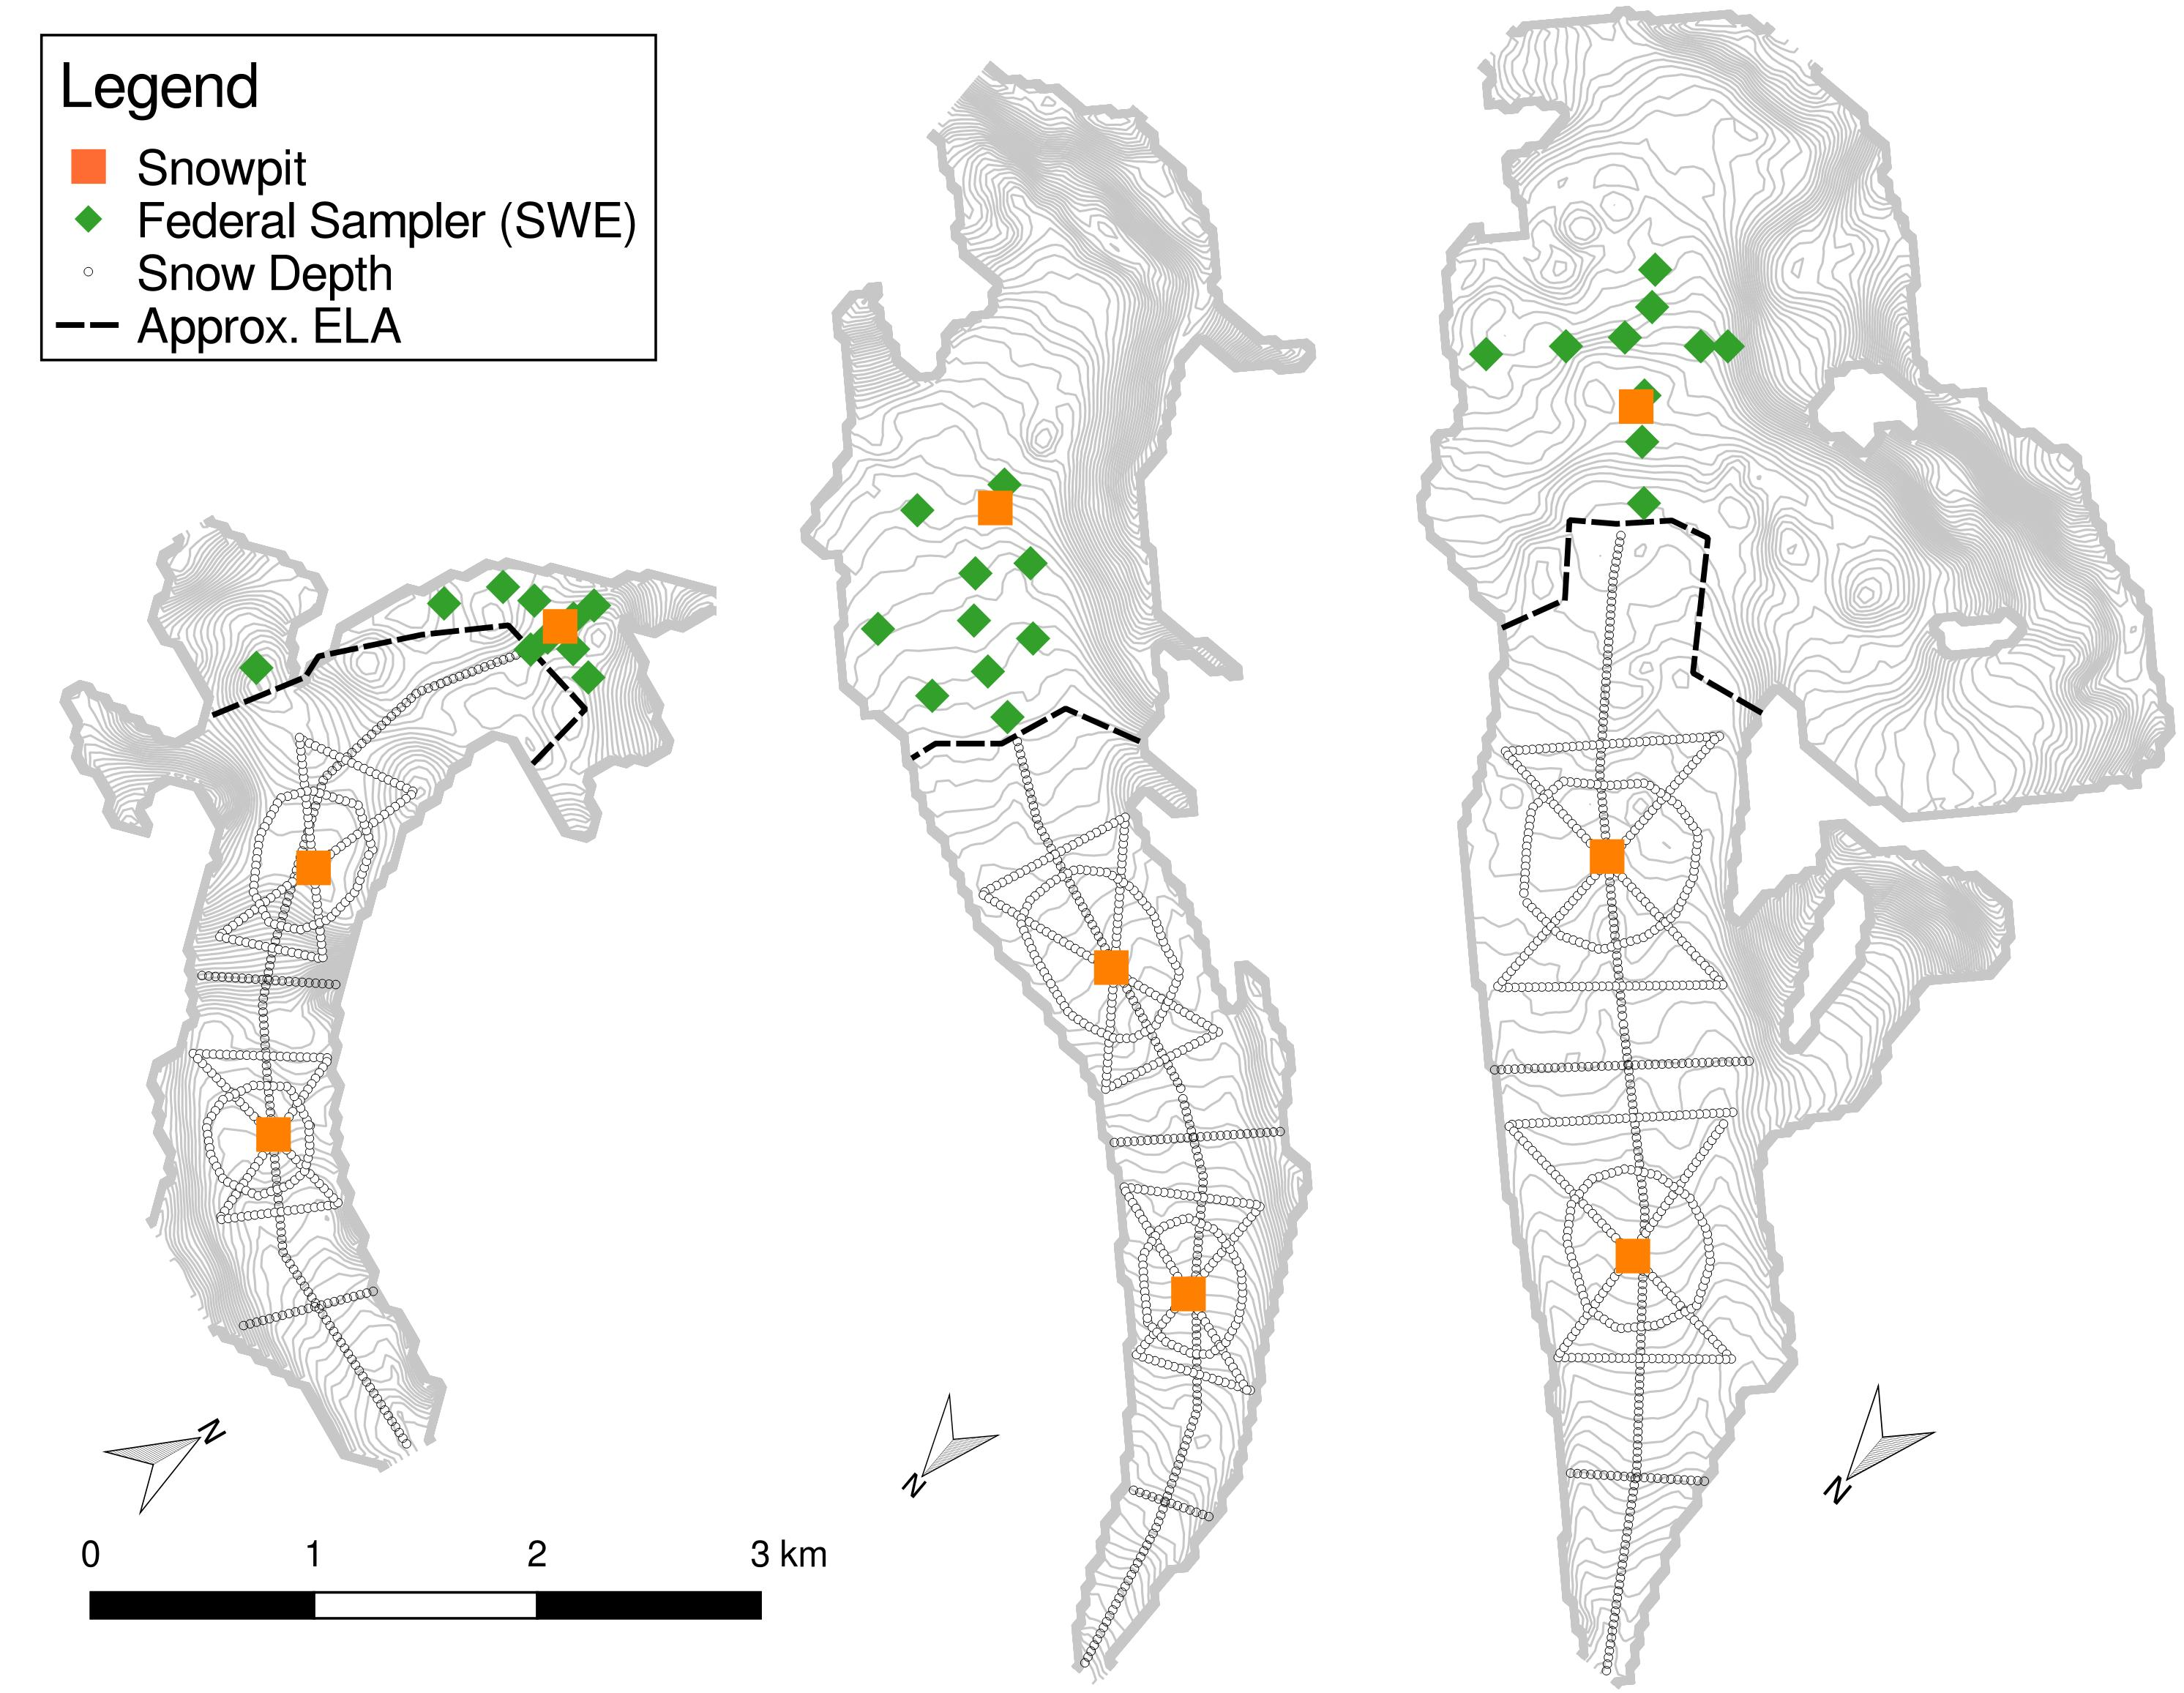
\includegraphics[height = 0.95\textwidth]{Transects_planned.jpeg}}\\
	\caption{Target waypoints for snow depth transects, snow pits, and SWE measurements on three study glaciers.}
	\label{transect_planned}
	\end{figure}

\begin{figure}
	\centering
	\fbox{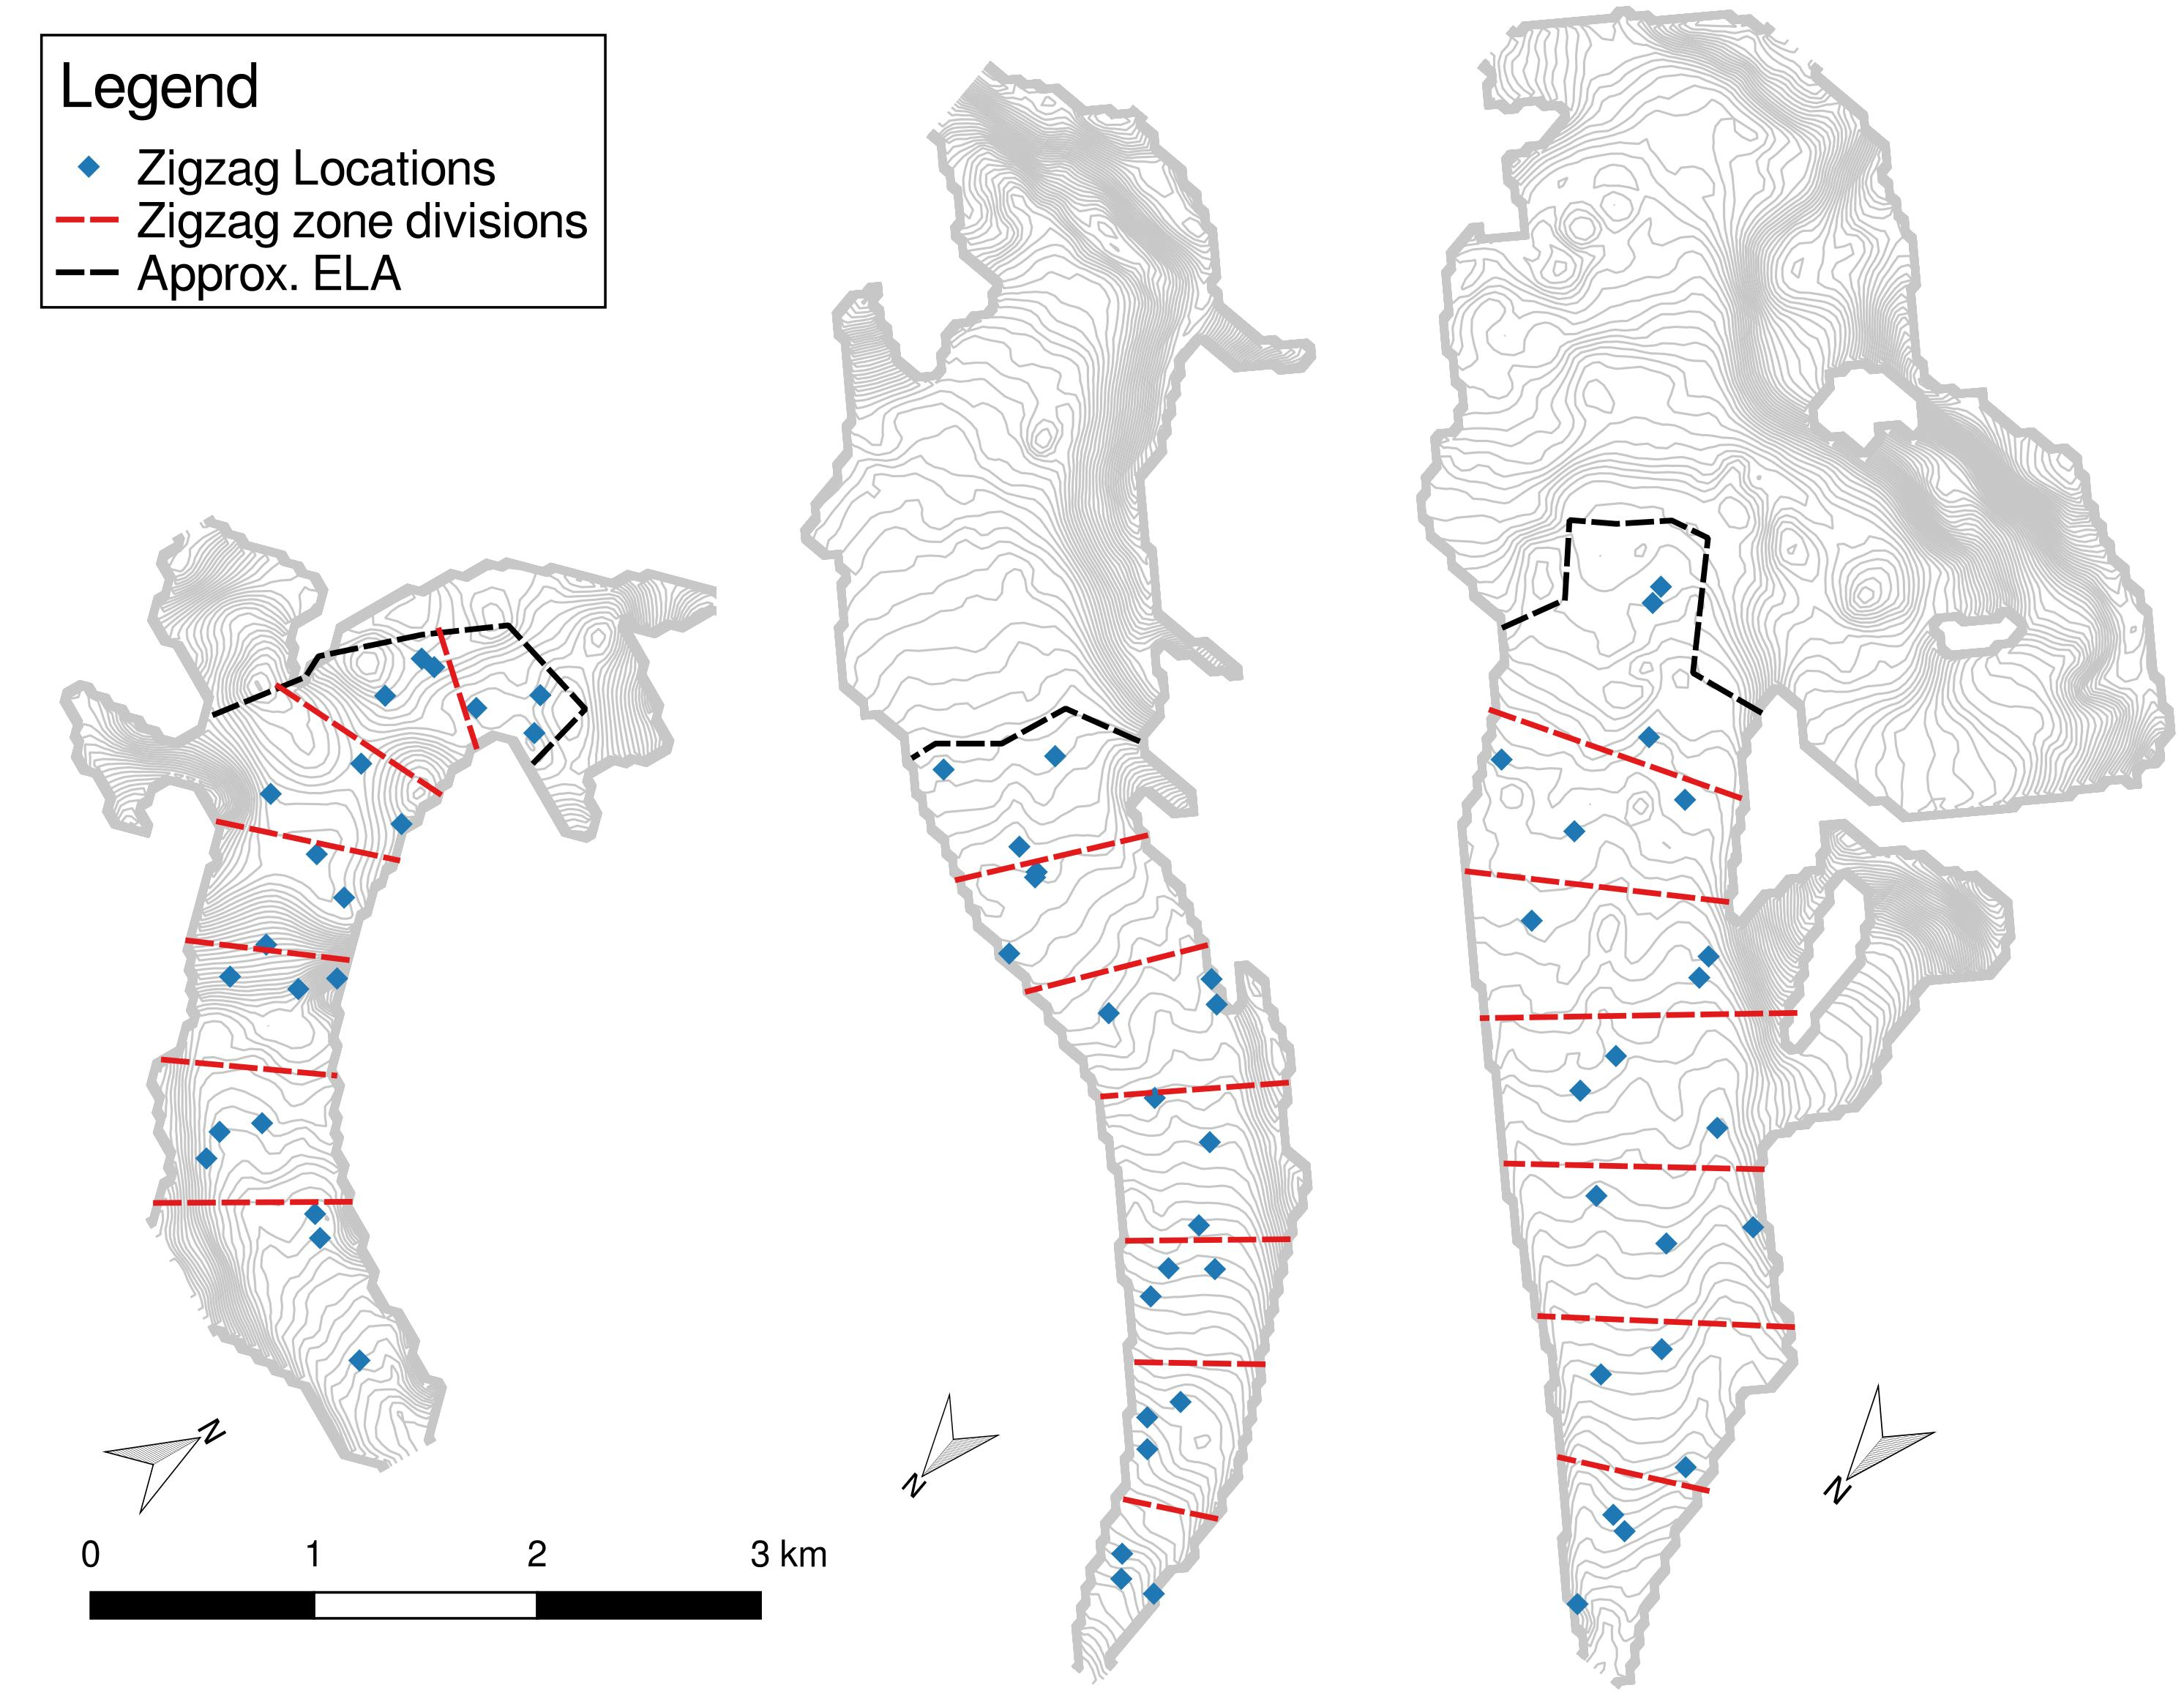
\includegraphics[height = 0.95\textwidth]{Zigzag_planned.jpeg}}\\
	\caption{Randomly assigned locations for zigzag measurements in the ablation area (divided into seven zones).}
	\label{zigzag_planned}
\end{figure}
\end{landscape}

\begin{figure}
	\centering
	\fbox{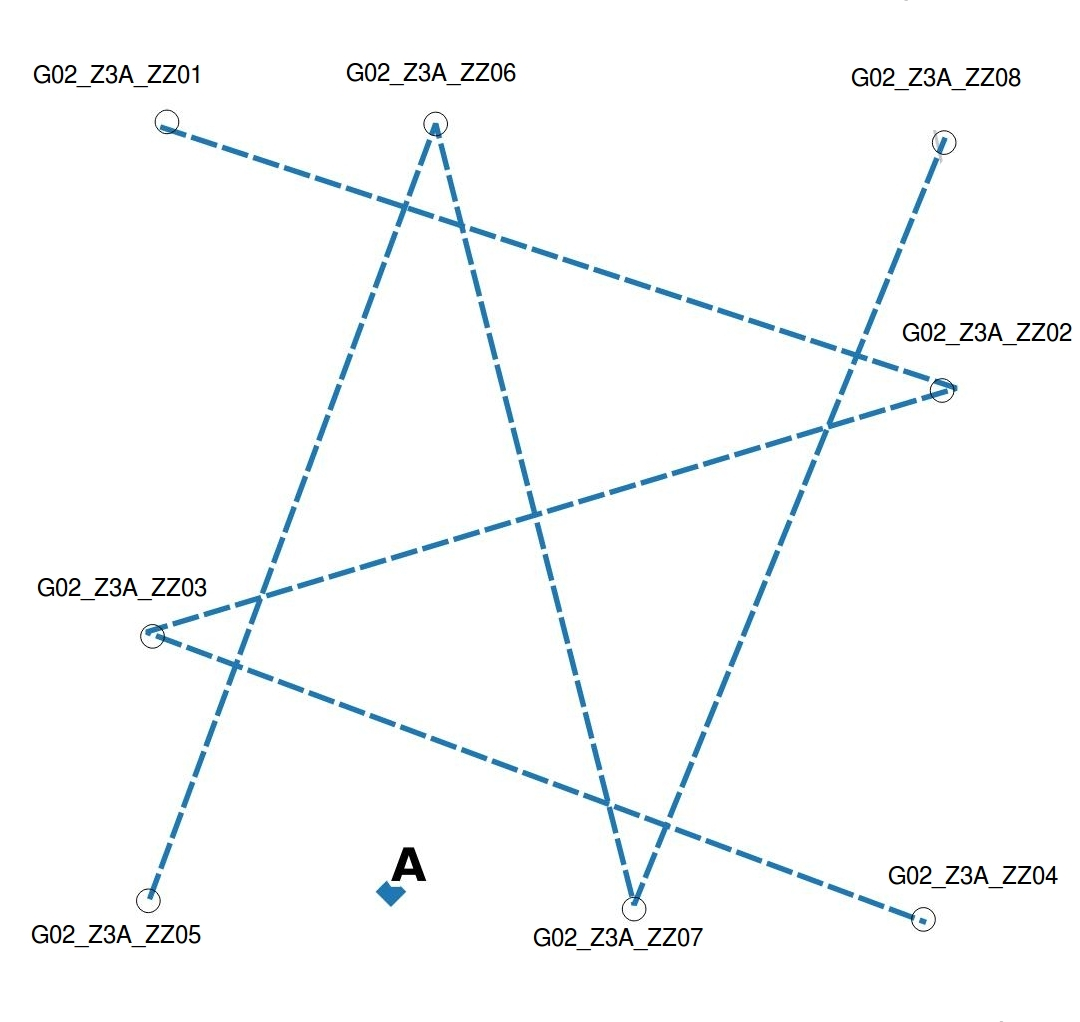
\includegraphics[height = 0.95\textwidth]{ZZ_vertex.jpeg}}\\
	\caption{Example of zigzag. Vertices are labelled and measurements are taken at random intervals along the dashed lines between vertices. The randomly chosen location of the SWE measurement is shown as a diamond.}
	\label{zigzag_vertex}
\end{figure}


%%%%
\section{Implementation}
%%%%

\subsection{Linear and Curvilinear Transects}
\label{sec:transects}

The transects, which include the hourglass, circle, transverse transect, and midline, were all executed in a similar way. Along each transect, waypoints were marked every 30 m. To sample these locations, a team of four people was used in the configuration shown in Figure \ref{photo_probing} and schematically in Figure \ref{probing}. The four people were roped together so that during typical glacier travel there was approximately 10 m separating each person (likely ranged between 9.5 and 11 m). The front person was responsible for navigation and waypoint marking and would follow these steps for each measurement location:
\begin{enumerate}
\item Use the GPS device to locate each intended waypoint
\item Navigate to that location using the GPS device
\item Stop and inform the team when they had arrived at the location
\item Mark a new waypoint on the GPS device as the real location of the measurement (allow for auto labelling of waypoint, which was a three digit number that increased by one with subsequent waypoints). When needed, call out the waypoint label to the team.
\item In one line of a field book, write the labels `Intended' for the waypoint that was being navigated to (code created during planning stage), `Real' for the name of the newly created waypoint on the GPS device (three digit number), as well as the easting, northing, and elevation for that location. This served as the backup for locating measurement points in the event of GPS device failure. 
\end{enumerate}

The remaining three people took snow depth measurement using a graduated 3.2 m avalanche probe. Upon arriving at the waypoint they would follow these steps:
\begin{enumerate}
\item Insert the probe into the snow until the snow/ice interface was reached. Read the depth of the snow pack on the probe to 0.5 cm. Repeat two (or three) more times (total of three (or four) measurements) within a 1 m$^2$ area of the first measurement and in a way that the three (or four) measurements are approximately equidistant. 
\item In one line of a field book, record the `Real' waypoint label (three digit number), as well as the three (or four) depth measurements. 
\end{enumerate}
Note that the snow/ice interface could often be differentiated from an ice lens. Typically, glacier ice felt hard, had a thin, low density (empty feeling) layer above, and created a bright `ping' sound in the probe. Ice lenses felt sticky and the probe would make a dull `thud' sound. In some locations this differentiation was obvious while in other locations it was difficult to be determine what was at the end of the probe. Often, layers in the snowpack could be felt with the probe. For example, the probe would move easily through low density layers such as depth hoar and would `stick' to hard layers or ice lenses. Increasing the force applied to the probe would usually allow the probe to penetrate through hard layers. In cases where the `sticky' layer could not be penetrated, the observer would place a question mark next to the recorded depth or simply omit that measurement. A question mark was also placed beside measurements that were notably smaller than adjacent measurements, which suggested much deeper snow. Note that the probe was inserted vertically, which was not necessarily perpendicular to the snow surface.

It was originally planned for each observer to take four depth measurements in a square pattern. However, during the first transect the observers found time consuming and difficult to remember and record four depths. The observers found that the most efficient way to collect data was to take three depth measurements, remember the values, and then write them all down in the field book. When four measurements were taken it was too difficult to remember all the values simultaneously so the whole process would take much longer. The decision was made to decrease the number of measurements so that we could increase the number of locations measured. 

There were dedicated field books for each type of measurement rather than each observer. The first person had the `Navigation' field book, the second person had `Snow depth \#1', the third person had `Snow depth \#2', and the fourth person had `Snow depth \#3'. In this way, the location of each measured value can be inferred from its location relative to the navigation person (where the location was being recorded). For example, the `Snow depth \#3' value was located $\sim$30 m behind the waypoint location along the trajectory between the previous and current waypoint. This arrangement was preferred to having a field book for each observer because it minimized confusion and potential errors when entering and processing data.

In this arrangement, snow depth measurements could be taken every 10 m along a transect if a waypoint was marked every 30 m. For the first two transects, measurements were completed at every waypoint. However, this also proved to be too time consuming so measurements were taken at every second waypoint for subsequent transects (exceptions include the midline on Glacier 4 and the lower hourglass on Glacier 2, see Table \ref{tab:snowdepthsummary}). A schematic of this arrangement can be seen in Figure \ref{probing:mapview}. Waypoints that were too dangerous to access were omitted. Additional waypoints (not originally uploaded to GPS devices) were created in some instances when travelling from the last accessible waypoint to the next accessible waypoint. A summary of information about the completed snow depth transects can be seen in Table \ref{tab:snowdepthsummary}.

\begin{figure}
	\centering
	\fbox{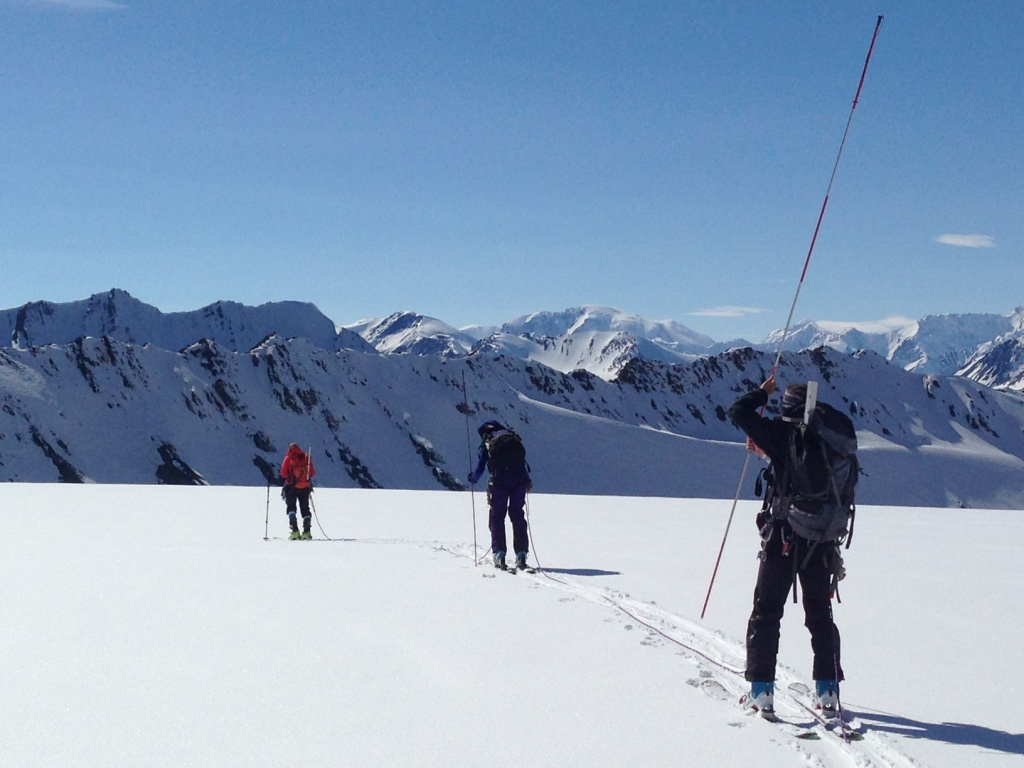
\includegraphics[width = 0.95\textwidth]{photo_probing.jpg}}\\
	\caption{Implementation of transect probing. The first person navigated to the intended waypoint using the GPS device. The second, third, and fourth (not seen) observers are probing using 3.2 m long avalanche probes. There is approximately 10 m between observers. Photo credit: G. Flowers}
	\label{photo_probing}
	\end{figure}


\begin{figure}
    \centering
    \begin{subfigure}[b]{0.8\textwidth}
        \fbox{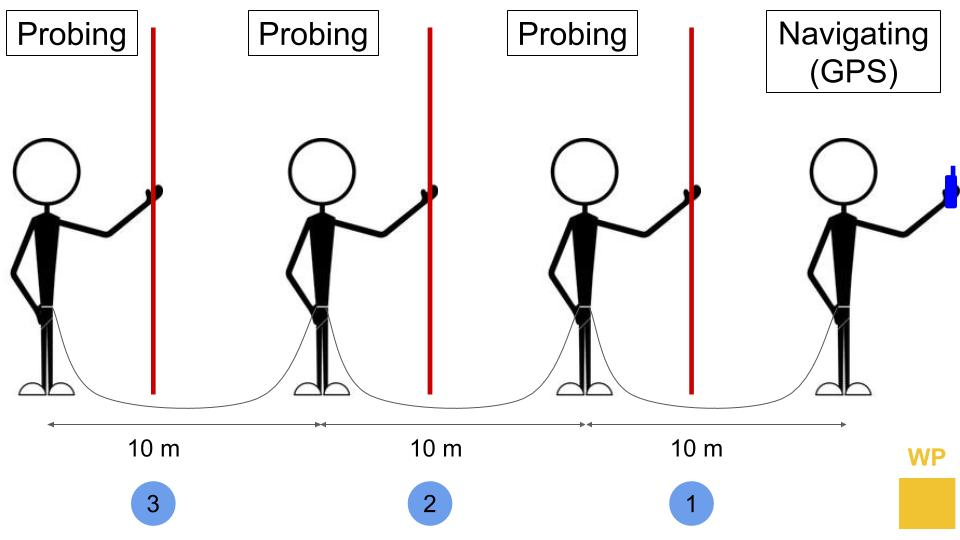
\includegraphics[width=\textwidth]{probers1.jpg}}
        \caption{Relative location of four people taking depth measurements at desired locations.}
        \label{probing:people}
    \end{subfigure}
    
    \begin{subfigure}[b]{0.8\textwidth}
        \fbox{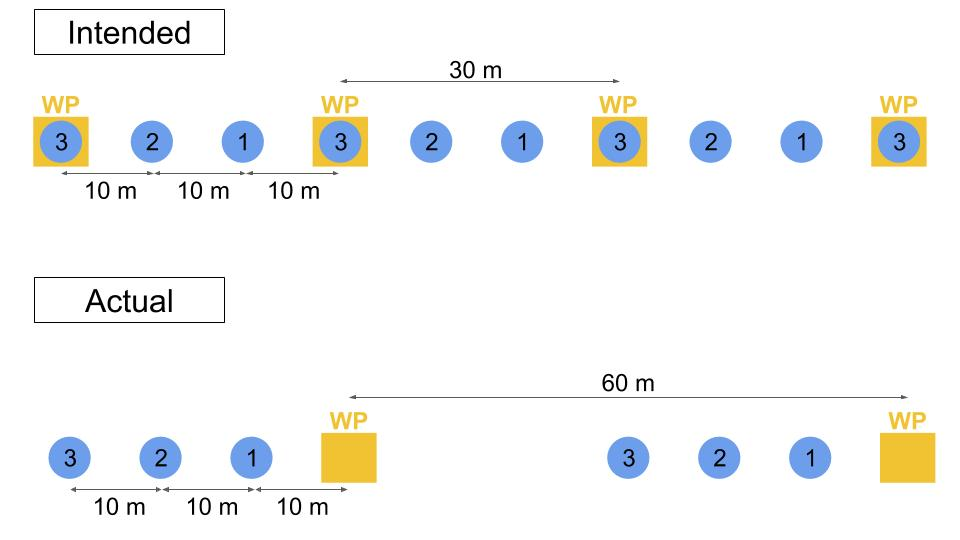
\includegraphics[width=\textwidth]{probers2.jpg}}
        \caption{Intended and actual transect depth measurement spacing. In the intended design, there was continuous measurement with 10 m sampling interval. In the actual implementation, every second waypoint was accessed so there was 60 m between subsequent measurements.}
        \label{probing:mapview}
    \end{subfigure}

    \caption{Schematic of the snow depth measurement configuration. Blue circles indicate depth measurement and orange squares indicate waypoint (WP) location.}\label{probing}
\end{figure}

\begin{landscape}

\begin{table}[]
\footnotesize
\centering
\caption{Summary information for snow depth transects. Transect shapes completed include Lower Hourglass (LH), Lower Circle (LC), Lower Midline (LM), Upper Hourglass (UH), Upper Circle (UC), Upper Midline (UM), Upper Transect (UT), and Bonus Transect (BT). The first observer was navigating to waypoints and the remaining three were taking depth measurements.}
\label{tab:snowdepthsummary}
\begin{tabular}{ccccccl}

\textbf{Glacier}                                                             & \textbf{Shape}                                               & \textbf{\begin{tabular}[c]{@{}c@{}}Measurement\\ Interval\end{tabular}}  & \textbf{Date} & \textbf{\begin{tabular}[c]{@{}c@{}}GPS \\ Waypoint\\  Labels\end{tabular}} & \textbf{\begin{tabular}[c]{@{}c@{}}Observer\\  Order\end{tabular}} & \multicolumn{1}{c}{\textbf{Comments}}                                                                                                                                                                                                            \\ \hline
\multirow{7}{*}{\begin{tabular}[c]{@{}c@{}}Glacier 4\\ (G04)\end{tabular}}   & \textbf{LH}                                                  & \begin{tabular}[c]{@{}c@{}}30 m \\ (60 m for \\ upper part)\end{tabular} & 4 May 2016    & 021 -- 070                                                                 & GF--AP--CA--AC                                                     & \begin{tabular}[c]{@{}l@{}}4 depth measurement/location \\ along upper part\end{tabular}                                                                                                                                                         \\
                                                                             & \textbf{LC}                                                  & 60 m                                                                     & 6 May 2016    & 159 -- 184                                                                 & GF--AP--CA--AC                                                     &                                                                                                                                                                                                                                                  \\
                                                                             & \textbf{LM}                                                  & 90 m                                                                     & 7 May 2016    & 185 -- 207                                                                 & AP--GF--CA--AC                                                     &                                                                                                                                                                                                                                                  \\
                                                                             & \textbf{UH}                                                  & 60 m                                                                     & 5 May 2016    & 072 -- 126                                                                 & CA--GF--AP--AC                                                     &                                                                                                                                                                                                                                                  \\
                                                                             & \textbf{UC}                                                  & 60 m                                                                     & 5 May 2016    & 127 -- 157                                                                 & CA--GF--AP--AC                                                     &                                                                                                                                                                                                                                                  \\
                                                                             & \textbf{UM}                                                  & 90 m                                                                     & 7 May 2016    & 208 -- 221                                                                 & AP--GF--CA--AC                                                     & Additional measurement at WP 158 (6 May 2016)                                                                                                                                                                                                               \\
                                                                             & \textbf{UT}                                                  & 30 m                                                                     & 4 May 2016    & 004 -- 020                                                                 & GF--AP--CA--AC                                                     & 4 depth measurement/location                                                                                                                                                                                                                     \\ \hline
\multirow{7}{*}{\begin{tabular}[c]{@{}c@{}}Glacier 2 \\ (G02)\end{tabular}}  & \textbf{\begin{tabular}[c]{@{}c@{}}LH \\ \& LC\end{tabular}} & 30 m                                                                     & 11 May 2016   & 371 -- 518                                                                 & GF--AP--CA                                                         & \begin{tabular}[c]{@{}l@{}}Only two probers. Avoided crossing main \\ channel so LH \& LC were combined and \\ done together on glacier right and then \\ glacier left of the channel. Almost all \\ measurements in the dune area.\end{tabular} \\
                                                                             & \textbf{LM}                                                  & $\sim$60 m                                                               & 10 May 2016   & 355 -- 370                                                                 & AP--GF--CA--AC                                                     & \begin{tabular}[c]{@{}l@{}}Original points along supraglacial stream \\ bed so points moved to glacier right and \\ locations were approximated\end{tabular}                                                                                     \\
                                                                             & \textbf{UH}                                                  & 60 m                                                                     & 8 May 2016    & 223 -- 275                                                                 & AC--AP--CA--GF                                                     & \begin{tabular}[c]{@{}l@{}}Many corner points avoided due to \\ crevasse danger\end{tabular}                                                                                                                                                     \\
                                                                             & \textbf{UC}                                                  & 60 m                                                                     & 8 May 2016    & 276 -- 313                                                                 & AC--AP--CA--GF                                                     &                                                                                                                                                                                                                                                  \\
                                                                             & \textbf{UM}                                                  & 60 m                                                                     & 9 May 2016    & 313 -- 343                                                                 & AC--AP--CA--GF                                                     &                                                                                                                                                                                                                                                  \\
                                                                             & \textbf{UT}                                                  & 60 m                                                                     & 11 May 2016   & 519 -- 528                                                                 & GF--AP--CA                                                         & Only two probers                                                                                                                                                                                                                                 \\
                                                                             & \textbf{BT}                                                  & $\sim$60 m                                                               & 19 May 2016   & 344 -- 354                                                                 & GF--AP--CA--AC                                                     &                                                                                                                                                                                                                                                  \\ \hline
\multirow{7}{*}{\begin{tabular}[c]{@{}c@{}}Glacier 13 \\ (G13)\end{tabular}} & \textbf{LH}                                                  & 60 m                                                                     & 15 May 2016   & 745 -- 811                                                                 & AC--AP--CA--GF                                                     &                                                                                                                                                                                                                                                  \\
                                                                             & \textbf{LC}                                                  & 60 m                                                                     & 15 May 2016   & 812 -- 847                                                                 & AC--AP--CA--GF                                                     &                                                                                                                                                                                                                                                  \\
                                                                             & \textbf{LM}                                                  & 60 m                                                                     & 14 May 2016   & 714 -- 743                                                                 & AC--AP--CA--GF                                                     &                                                                                                                                                                                                                                                  \\
                                                                             & \textbf{UH}                                                  & 60 m                                                                     & 12 May 2016   & 571 -- 650                                                                 & AC--GF--CA--AP                                                     &                                                                                                                                                                                                                                                  \\
                                                                             & \textbf{UC}                                                  & 60 m                                                                     & 12 May 2016   & 529 -- 570                                                                 & AC--GF--CA--AP                                                     &                                                                                                                                                                                                                                                  \\
                                                                             & \textbf{UM}                                                  & 60 m                                                                     & 14 May 2016   & 678 -- 713                                                                 & AC--AP--CA--GF                                                     &                                                                                                                                                                                                                                                  \\
                                                                             & \textbf{UT}                                                  & 60 m                                                                     & 14 May 2016   & 660 -- 677                                                                 & AC--AP--CA--GF                                                     &                                                                                                                                                                                                                                                 
\end{tabular}
\end{table}

\normalsize
\begin{table}[]
\centering
\caption{Summary information for zigzag measurements}
\label{tab:zigzagsummary}
\begin{tabular}{cccccl}
\textbf{Glacier} & \textbf{Zone} & \textbf{Priority} & \textbf{Date} & \textbf{Observers} & \multicolumn{1}{c}{\textbf{Comments}}                                                                          \\ \hline
G04              & 3             & A                 & 5 May 2016    & AP/CA              &                                                                                                                \\
G04              & 2             & A                 & 7 May 2016    & CA/AC              &                                                                                                                \\
G04              & 5             & B                 & 7 May 2016    & AP/GF              & \begin{tabular}[t]{@{}l@{}}Sticky layer - many points not collected\\ Snowing during measurements\end{tabular} \\ \hline
G02              & 5             & C                 & 10 May 2016   & CA/GF              & \begin{tabular}[t]{@{}l@{}}Extra line measured\\ Vertex labelling error in GPS device \end{tabular}                                                                                   \\
G02              & 7             & A                 & 10 May 2016   & CA/GF/AP/AC              & \begin{tabular}[t]{@{}l@{}}Channel present\\ Vertex labelling error in GPS device\end{tabular}                        \\
G02              & 3             & B                 & 10 May 2016   & GF/AP              & Vertex labelling error in GPS device                                                                                  \\ \hline
G13              & 7             & C                 & 14 May 2016   & AC/AP              & Vertex labelling error in GPS device                                                                                  \\
G13              & 4             & C                 & 14 May 2016   & GF/CA              & \begin{tabular}[t]{@{}l@{}}Channel present\\ Vertex labelling error in GPS device\end{tabular}                        \\
G13              & 3             & B                 & 15 May 2016   & GF/CA              & Vertex labelling error in GPS device                                                                                  \\
G13              & 5             & A                 & 15 May 2016   & AP/AC              & \begin{tabular}[t]{@{}l@{}}Mushy snow that collapses\\ Vertex labelling error in GPS device\end{tabular}             
\end{tabular}
\end{table}

 \begin{figure}
	\centering
	\fbox{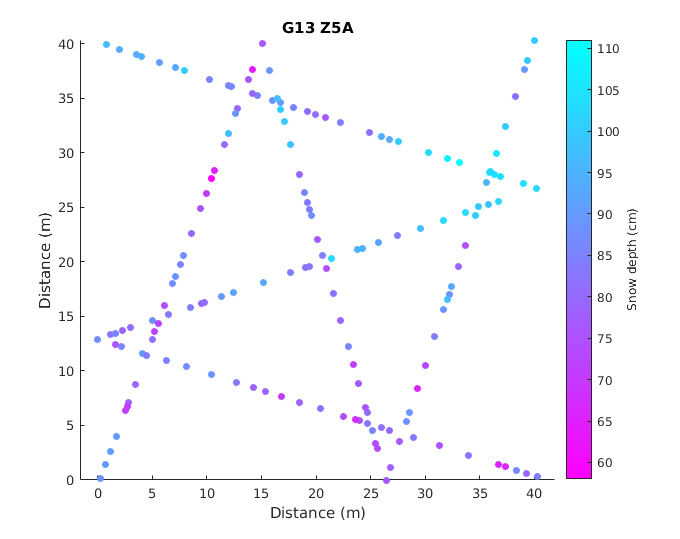
\includegraphics[height = \textwidth]{zigzag_completed.png}}\\
	\caption{Snow depth values measured along a zigzag pattern (G04\_Z3A)}
	\label{zigzag_example}
\end{figure}

\end{landscape}

\begin{table}[]
\centering
\caption{Summary information for SWE measurements with the Federal Snow Sampler}
\label{tab:SWEsummary}
\begin{tabular}{ccccccl}
\textbf{Glacier}      & \textbf{Location} & \textbf{\begin{tabular}[c]{@{}c@{}}Total\\ Values\end{tabular}} & \textbf{\begin{tabular}[c]{@{}c@{}}Number \\ of Tube \\ Lengths\end{tabular}} & \textbf{Date} & \textbf{Observers} & \multicolumn{1}{c}{\textbf{Comments}}                                        \\ \hline
\multirow{7}{*}{G04}  & Z3A               & 5                                                               & 3                                                                             & 5 May 2016    & GF/AC              &                                                                              \\
                      & USP               & 2+2+2+3                                                         & 3                                                                             & 5 May 2016    & GF/CA              &                                                                              \\
                      & Z2A               & 3                                                               & 3                                                                             & 7 May 2016    & GF/AP              &                                                                              \\
                      & LSP               & 3+2+2+2                                                         & 3                                                                             & 7 May 2016    & GF/CA              &                                                                              \\
                      & Z5B               & 3                                                               & 3                                                                             & 7 May 2016    & CA/AC              &                                                                              \\
                      & Z5A               & 3                                                               & 3                                                                             & 7 May 2016    & CA/AC              &                                                                              \\
                      & Z5C               & 3                                                               & 2                                                                             & 7 May 2016    & CA/AC              &                                                                              \\ \hline
\multirow{7}{*}{G02}  & Z5C               & 3                                                               & 2                                                                             & 10 May 2016   & AP/AC              &                                                                              \\
                      & USP               & 3+2+2+2                                                         & 2                                                                             & 10 May 2016   & AP/AC              &                                                                              \\
                      & Z7A               & 3                                                               & 3                                                                             & 10 May 2016   & CA/GF              &                                                                              \\
                      & Z7B               & 3                                                               & 3                                                                             & 10 May 2016   & CA/GF              &                                                                              \\
                      & Z7C               & 3                                                               & 2                                                                             & 10 May 2016   & AP/CA              &                                                                              \\
                      & LSP               & 2+2+2+2                                                         & 1                                                                             & 10 May 2016   & CA/AC              & \begin{tabular}[t]{@{}l@{}}Used snowpit \\ spring scale (grams)\end{tabular} \\
                      & Z3B               & 3                                                               & 1                                                                             & 10 May 2016   & CA/AC              & \begin{tabular}[t]{@{}l@{}}Used snowpit \\ spring scale (grams)\end{tabular} \\ \hline
\multirow{19}{*}{G13} & ASP               & 2+2+2+2                                                         & 3                                                                             & 13 May 2016   & AP/AC              &                                                                              \\
                      & AFC05             & 3                                                               & 3                                                                             & 13 May 2016   & AP/CA              & \begin{tabular}[t]{@{}l@{}}Probe depth \\ $\neq$ tube depth\end{tabular}     \\
                      & WP 651            & 3                                                               & 3                                                                             & 13 May 2016   & AP/CA/GF           &                                                                              \\
                      & WP 652            & 4                                                               & 3                                                                             & 13 May 2016   & AP/CA/GF           &                                                                              \\
                      & WP 653            & 3                                                               & 3                                                                             & 13 May 2016   & AP/CA/GF           &                                                                              \\
                      & WP 654            & 3                                                               & 3                                                                             & 13 May 2016   & AP/CA/GF           &                                                                              \\
                      & WP 655            & 3                                                               & 3                                                                             & 13 May 2016   & AP/CA/GF           &                                                                              \\
                      & WP 656            & 3                                                               & 3                                                                             & 13 May 2016   & AP/CA/GF           &                                                                              \\
                      & WP 657            & 3                                                               & 3                                                                             & 13 May 2016   & AP/CA/GF           &                                                                              \\
                      & WP 658            & 3                                                               & 3                                                                             & 13 May 2016   & AP/CA/GF           &                                                                              \\
                      & WP 659            & 3                                                               & 3                                                                             & 13 May 2016   & AP/CA/GF           &                                                                              \\
                      & Z7C               & 3                                                               & 2                                                                             & 13 May 2016   & CA/GF              &                                                                              \\
                      & USP               & 2+2+2+2                                                         & 2                                                                             & 14 May 2016   & AP/AC              & \begin{tabular}[t]{@{}l@{}}Ice layer near \\ bottom\end{tabular}             \\
                      & Z4C               & 3                                                               & 3                                                                             & 14 May 2016   & AP                 & In stream channel                                                            \\
                      & WP 744            & 3                                                               & 2                                                                             & 14 May 2016   & AP                 & In Z4C zigzag                                                                \\
                      & Z3B               & 3                                                               & 2                                                                             & 15 May 2016   & AP/AC              &                                                                              \\
                      & Z4B               & 3                                                               & 2                                                                             & 15 May 2016   & AP/AC              &                                                                              \\
                      & Z5C               & 3                                                               & 2                                                                             & 15 May 2016   & CA/GF              &                                                                              \\
                      & Z5B               & 3                                                               & 2                                                                             & 15 May 2016   & CA/AC              &                                                                             
\end{tabular}
\end{table}



\subsection{Zigzag}

The zigzag sampling pattern was used to obtain many measurements within a 40 x 40 m area.  The pattern consisted of two intersecting `Z' shaped transects. Snow depth was measured with random spacing between 0.3 m and 3.0 m. 

Two teams of two people were used to complete each zigzag. The first team would navigate to the vertices of the zigzag using the GPS device and place wands at each vertex. Often the tracks would not be straight between two vertices so the second team would use the wands to travel between vertices in as straight a line as possible. The first person would use the avalanche probe to measure out the distance to the next measurement spot and then probe at that point (Sturm, M., 2016 personal communication). Probing protocol was exactly the same as for transect measurements (see Section \ref{sec:transects}). The first person would call out the depth to the second person, who was responsible for recording the distance between measurements and the depth at the measurement point. A field book was dedicated to zigzag measurements and each page would have the name of the vertex where measurements started, the distance from the previous measurement point and the depth at that point. The second person also had a sheet with random numbers from a uniform distribution between 0.3 and 3.0 m (generated used Matlab) and would call out these numbers in order as the distance between measurement points. While the second team was measuring snow depth, the first team took three SWE measurements with a $\sim$1 m area around the predetermined location within the zigzag area (see Section \ref{sec:SWE} for protocol). An example of a completed zigzag pattern can be seen in Figure \ref{zigzag_example} and a summary of information about completed zigzags can be seen in Table \ref{tab:zigzagsummary}.


 \subsection{Federal Snow Sampler}
\label{sec:SWE}
 
\begin{figure}
    \centering
    \begin{subfigure}[b]{0.38\textwidth}
        \fbox{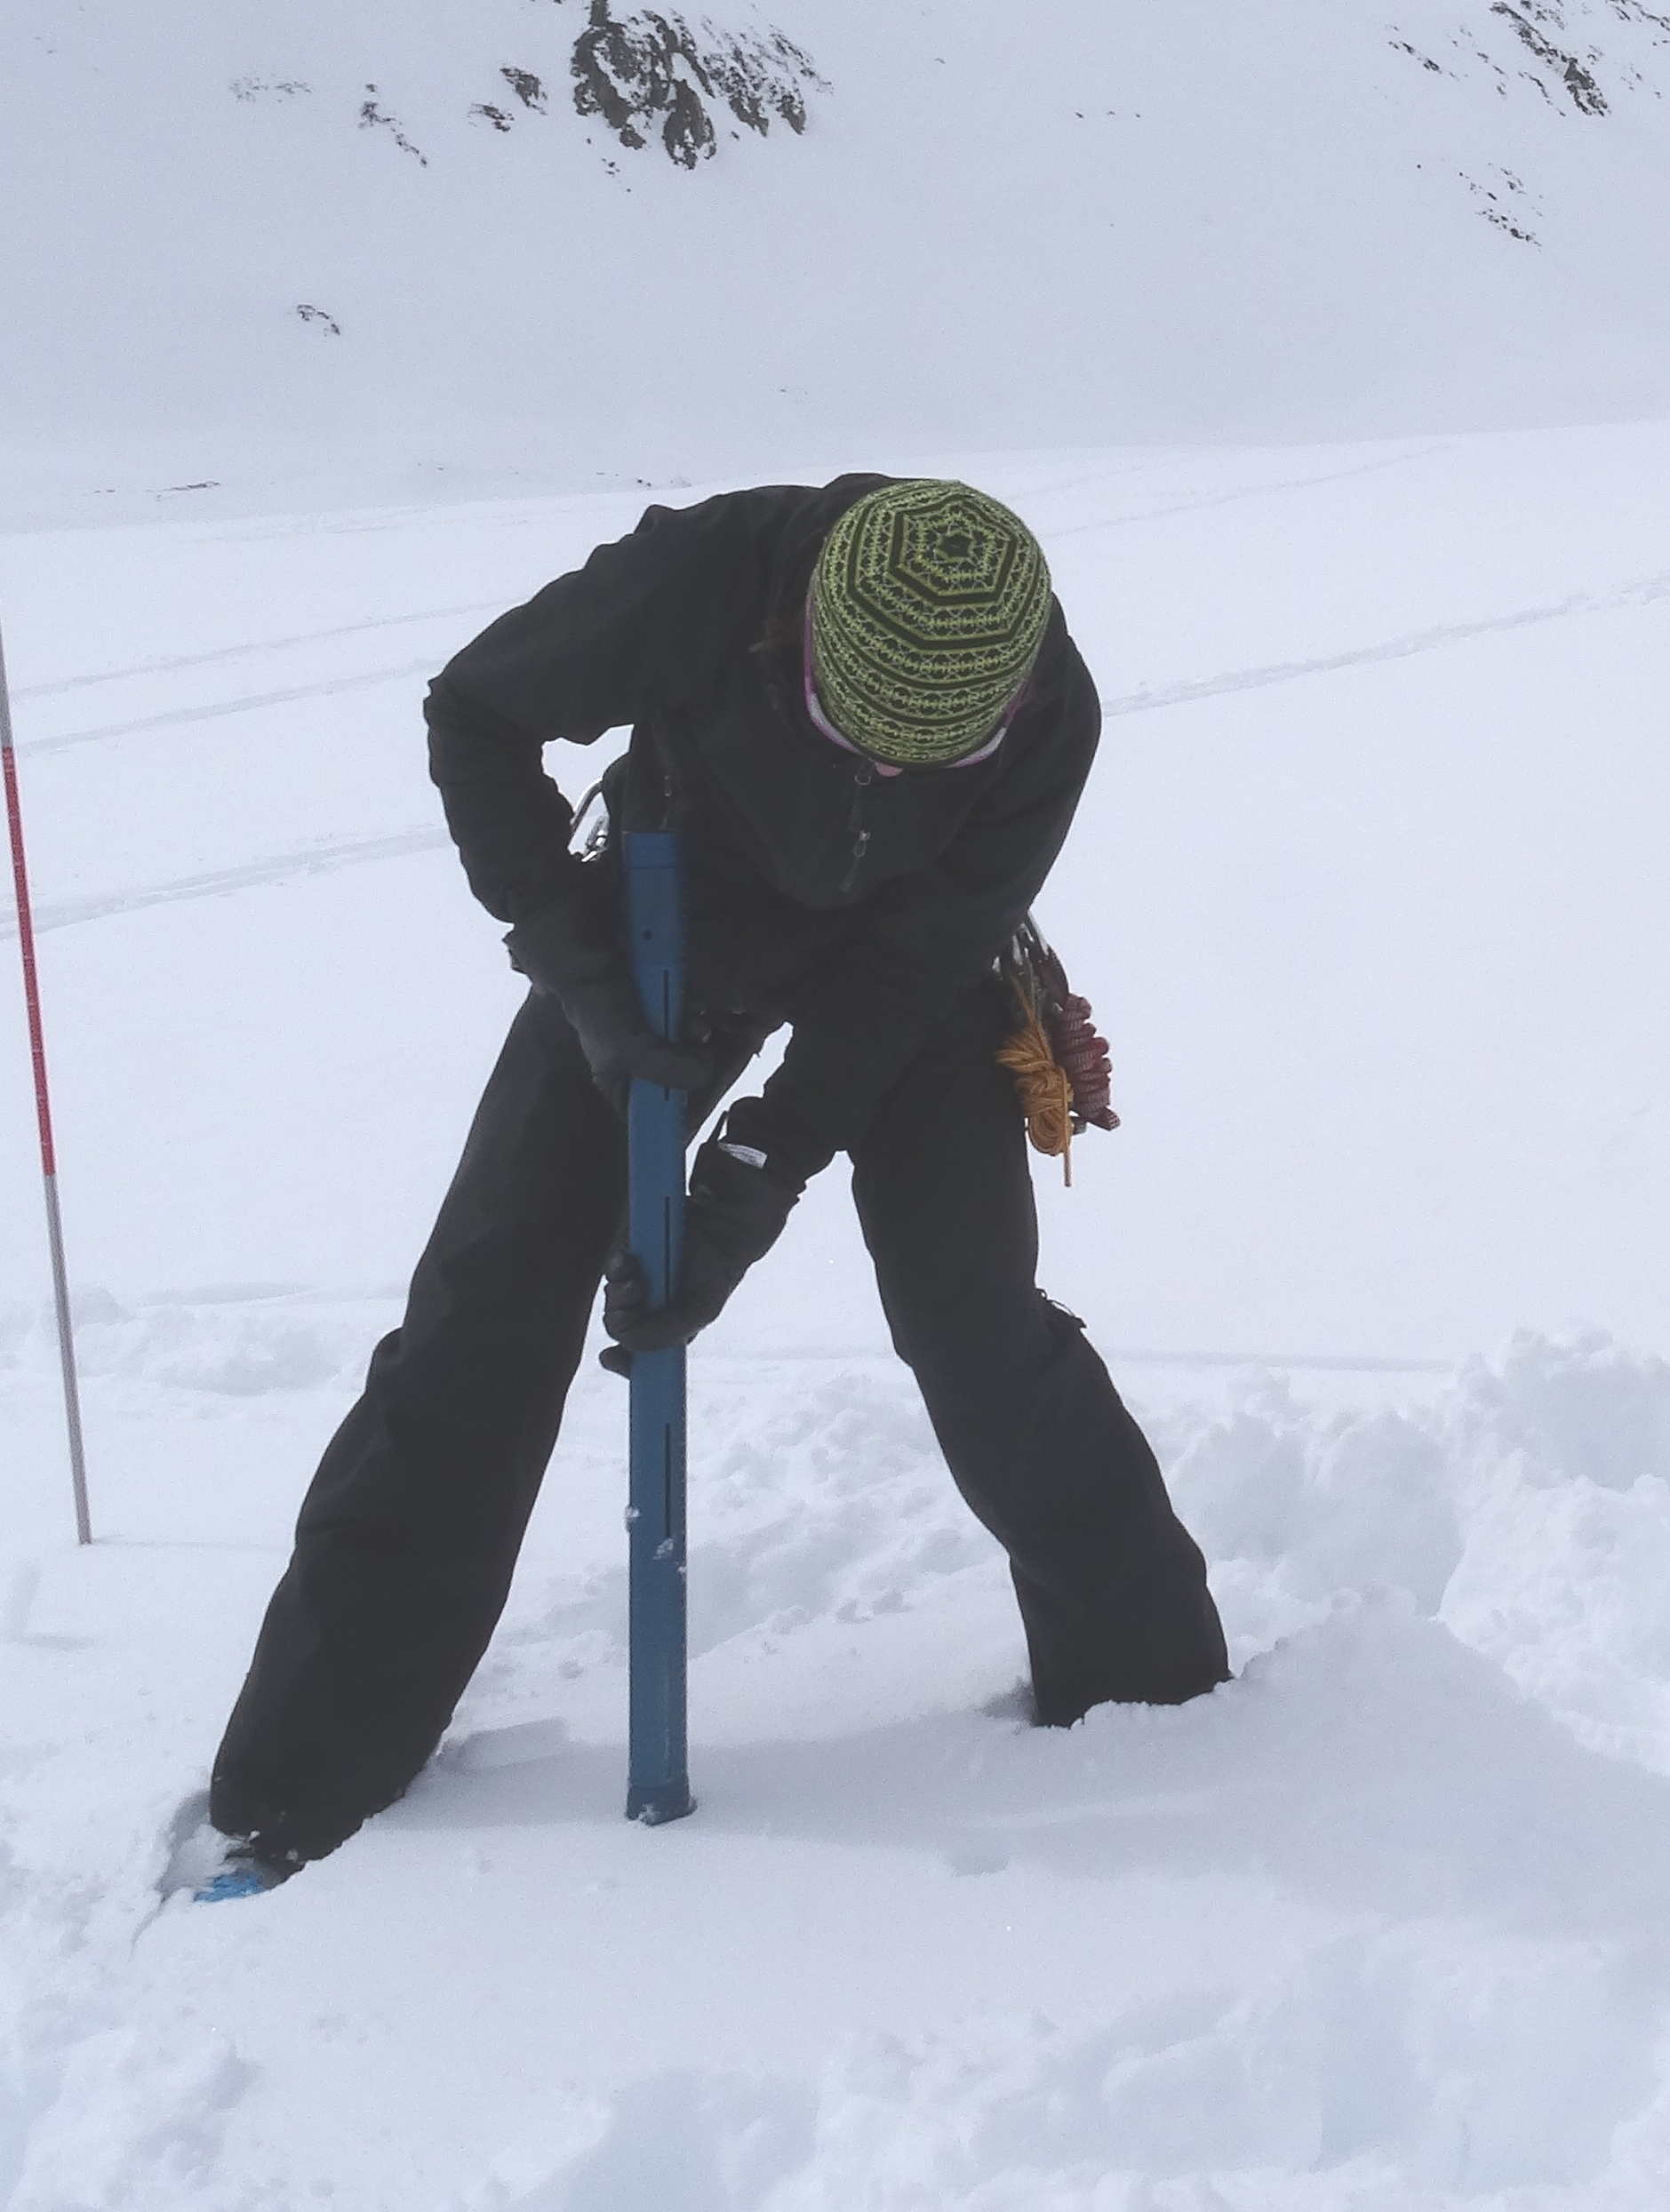
\includegraphics[width=\textwidth]{photo_swe1.JPG}}
        \caption{Inserting the Federal Sampler into the snow. Photo credit: C. Ariagno}
        \label{photo_swe1}
    \end{subfigure}
    ~
    \begin{subfigure}[b]{0.56\textwidth}
        \fbox{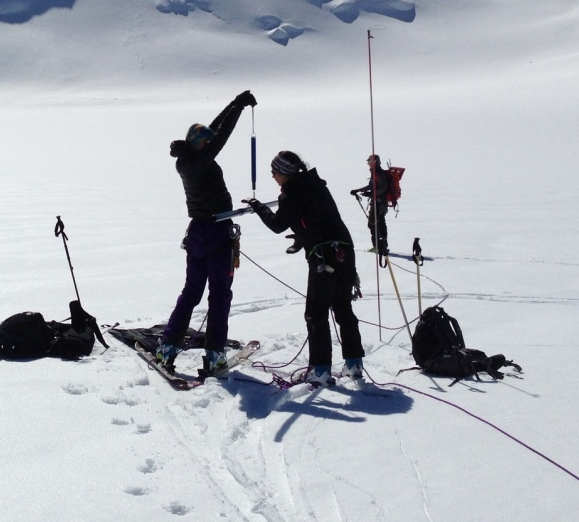
\includegraphics[width=\textwidth]{photo_swe2.jpg}}
        \caption{Weighing the Federal Sampler using the spring scale (units of cm SWE). Photo credit: G. Flowers}
        \label{photo_swe2}
    \end{subfigure}

    \caption{Using the Federal Sampler to measure SWE}
    \label{photo_swe}
\end{figure}
 
A metric Federal Snow Sampler from Geo Scientific Ltd. was used to measure snow depth and snow water equivalent (SWE). At the predetermined locations, three measurements (within 50 cm of each other) were made using the sampler. At the snowpit locations, a total of eight measurements were made, with two measurements on each side of the snowpit. Density calculated from these values will be compared with density determined from sampling within the snow pit (see Section \ref{sec:snowpit}). 

The Federal Snow Sampler consists of four 0.83 m sections that could be screwed together. One end of the sampler has cutter teeth and the other end has a removable thread protector that can be screwed onto the top section of the tube. The sampler has graduations in units of 1 cm and slits along the side of the tube allow the observer to determine the length of the core when it is in the tube. The spring scale that comes with the Federal Sampler is in units of cm SWE.  

To take a measurement with the Federal Sampler the following steps were taken:
\begin{enumerate}
\item Three depth measurements (within $\sim$50 cm of each other) were made using an avalanche probe and the depths were recorded.
\item The weight (in cm SWE) of the assembled empty tube was measured using the spring scale and then recorded (tare).
\item The tube was placed vertically into the snow and then pushed and twisted clockwise so that the cutters at the end of the tube would penetrate the snow pack. If this proved to be too difficult, the T-handle was added onto the tube to aid in pushing the tube further into the snow. 
\item When the bottom of the snow pack was reached, the observer would measure the snow depth by using the graduation on the outside of the tube.
\item The tube was then gently pulled out of the snow (so as not to lose any snow from the bottom). The length of the snow core inside the tube was then measured by using the side slits to see the top of the core and lining it up with the graduation on the outside of the tube. This value was then recorded. If the length of the snow core was much less than the snow depth (typically a result of lost snow), the sample measurement was redone.
\item The snow and tube were weighed together using the spring scale and the value was recorded.
\item The tube was then emptied and wiped using a soft cloth on a pole to remove any moisture. 
\end{enumerate}

When the T-handle was used, the tube segments often became difficult to take apart. The small handles provided in the kit aided in disassembling the Federal Sampler. However, if a significant force was applied to the T-handle during sampling and the tube segments seized then longer handles (accomplished by attaching snow shovel handles to provided tools) helped in disassembling the sampler. Anti-seizing compound was included in the kit and was applied when needed. A summary of information about completed SWE measurements can be seen in Table \ref{tab:SWEsummary}.

\subsection{Firn Corer}

The firn corer was intended to be used in the accumulation area to extract a snow/firn core. The coring device would be beneficial in the accumulation area because the core can be extracted and used to determine the location of the snow/firn transition. From that, the snow depth and the mass of the snow core, which included only the past year of accumulation, could be determined. The Federal Sampler was thought to be ineffective in the accumulation area because the snow/firn transition may not have been felt and the core cannot be examined to establish where the transition occurs.

When the corer was used in the field however, a number of problems were encountered that prevented the collection of accurate measurements. The first was that the snow core would get stuck inside the core barrel. Warm temperatures meant that the barrel would get wet from snow melt and when it was inserted into the snow pack, the snow would freeze onto the side of the barrel. This meant that the core was destroyed in the extraction process. The second problem (which was connected to the first problem) was that the coring chips in the hole could not be discriminated from the core itself. Coring chips are loose snow crystals that fall to the bottom of the drilling hole when the barrel is taken out. When the barrel is reinserted for the second (or third) core, the snow in the subsequent core will contain these coring chips, which are not part of the intended core. The mass of the core will be incorrect (overestimate) because of this additional snow. This problem is typically avoided by extracting the in-tact core and identifying and removing the coring chips. However, since the core could not be extracted as one piece, this step was not possible and the masses of the cores were incorrect. 

In a few locations, sections of the core could be exacted without breaking them apart. In these areas the snow/firn transition could be identified. This means that in principal, the firn corer could be used to determine the depth of this transition. The main challenge is therefore being able to identify chips. In firn core trials that occurred after this field work, it was found that the the cores could be pulled out easily if the barrel was not totally full. However, in these less compacted cores the chips were difficult to identify so the problem persists. 

As a result of these complications, many accumulation area measurements on Glacier 4 and Glacier 2 were abandoned. On Glacier 13, the Federal Sampler was successfully used to take SWE measurements. The snow/firn transition could be felt with the Federal Sampler because of the large density change, which made it almost impossible to further insert the tube into the snow pack.  

\subsection{Snowpit}
\label{sec:snowpit}

\begin{figure}
	\centering
	\fbox{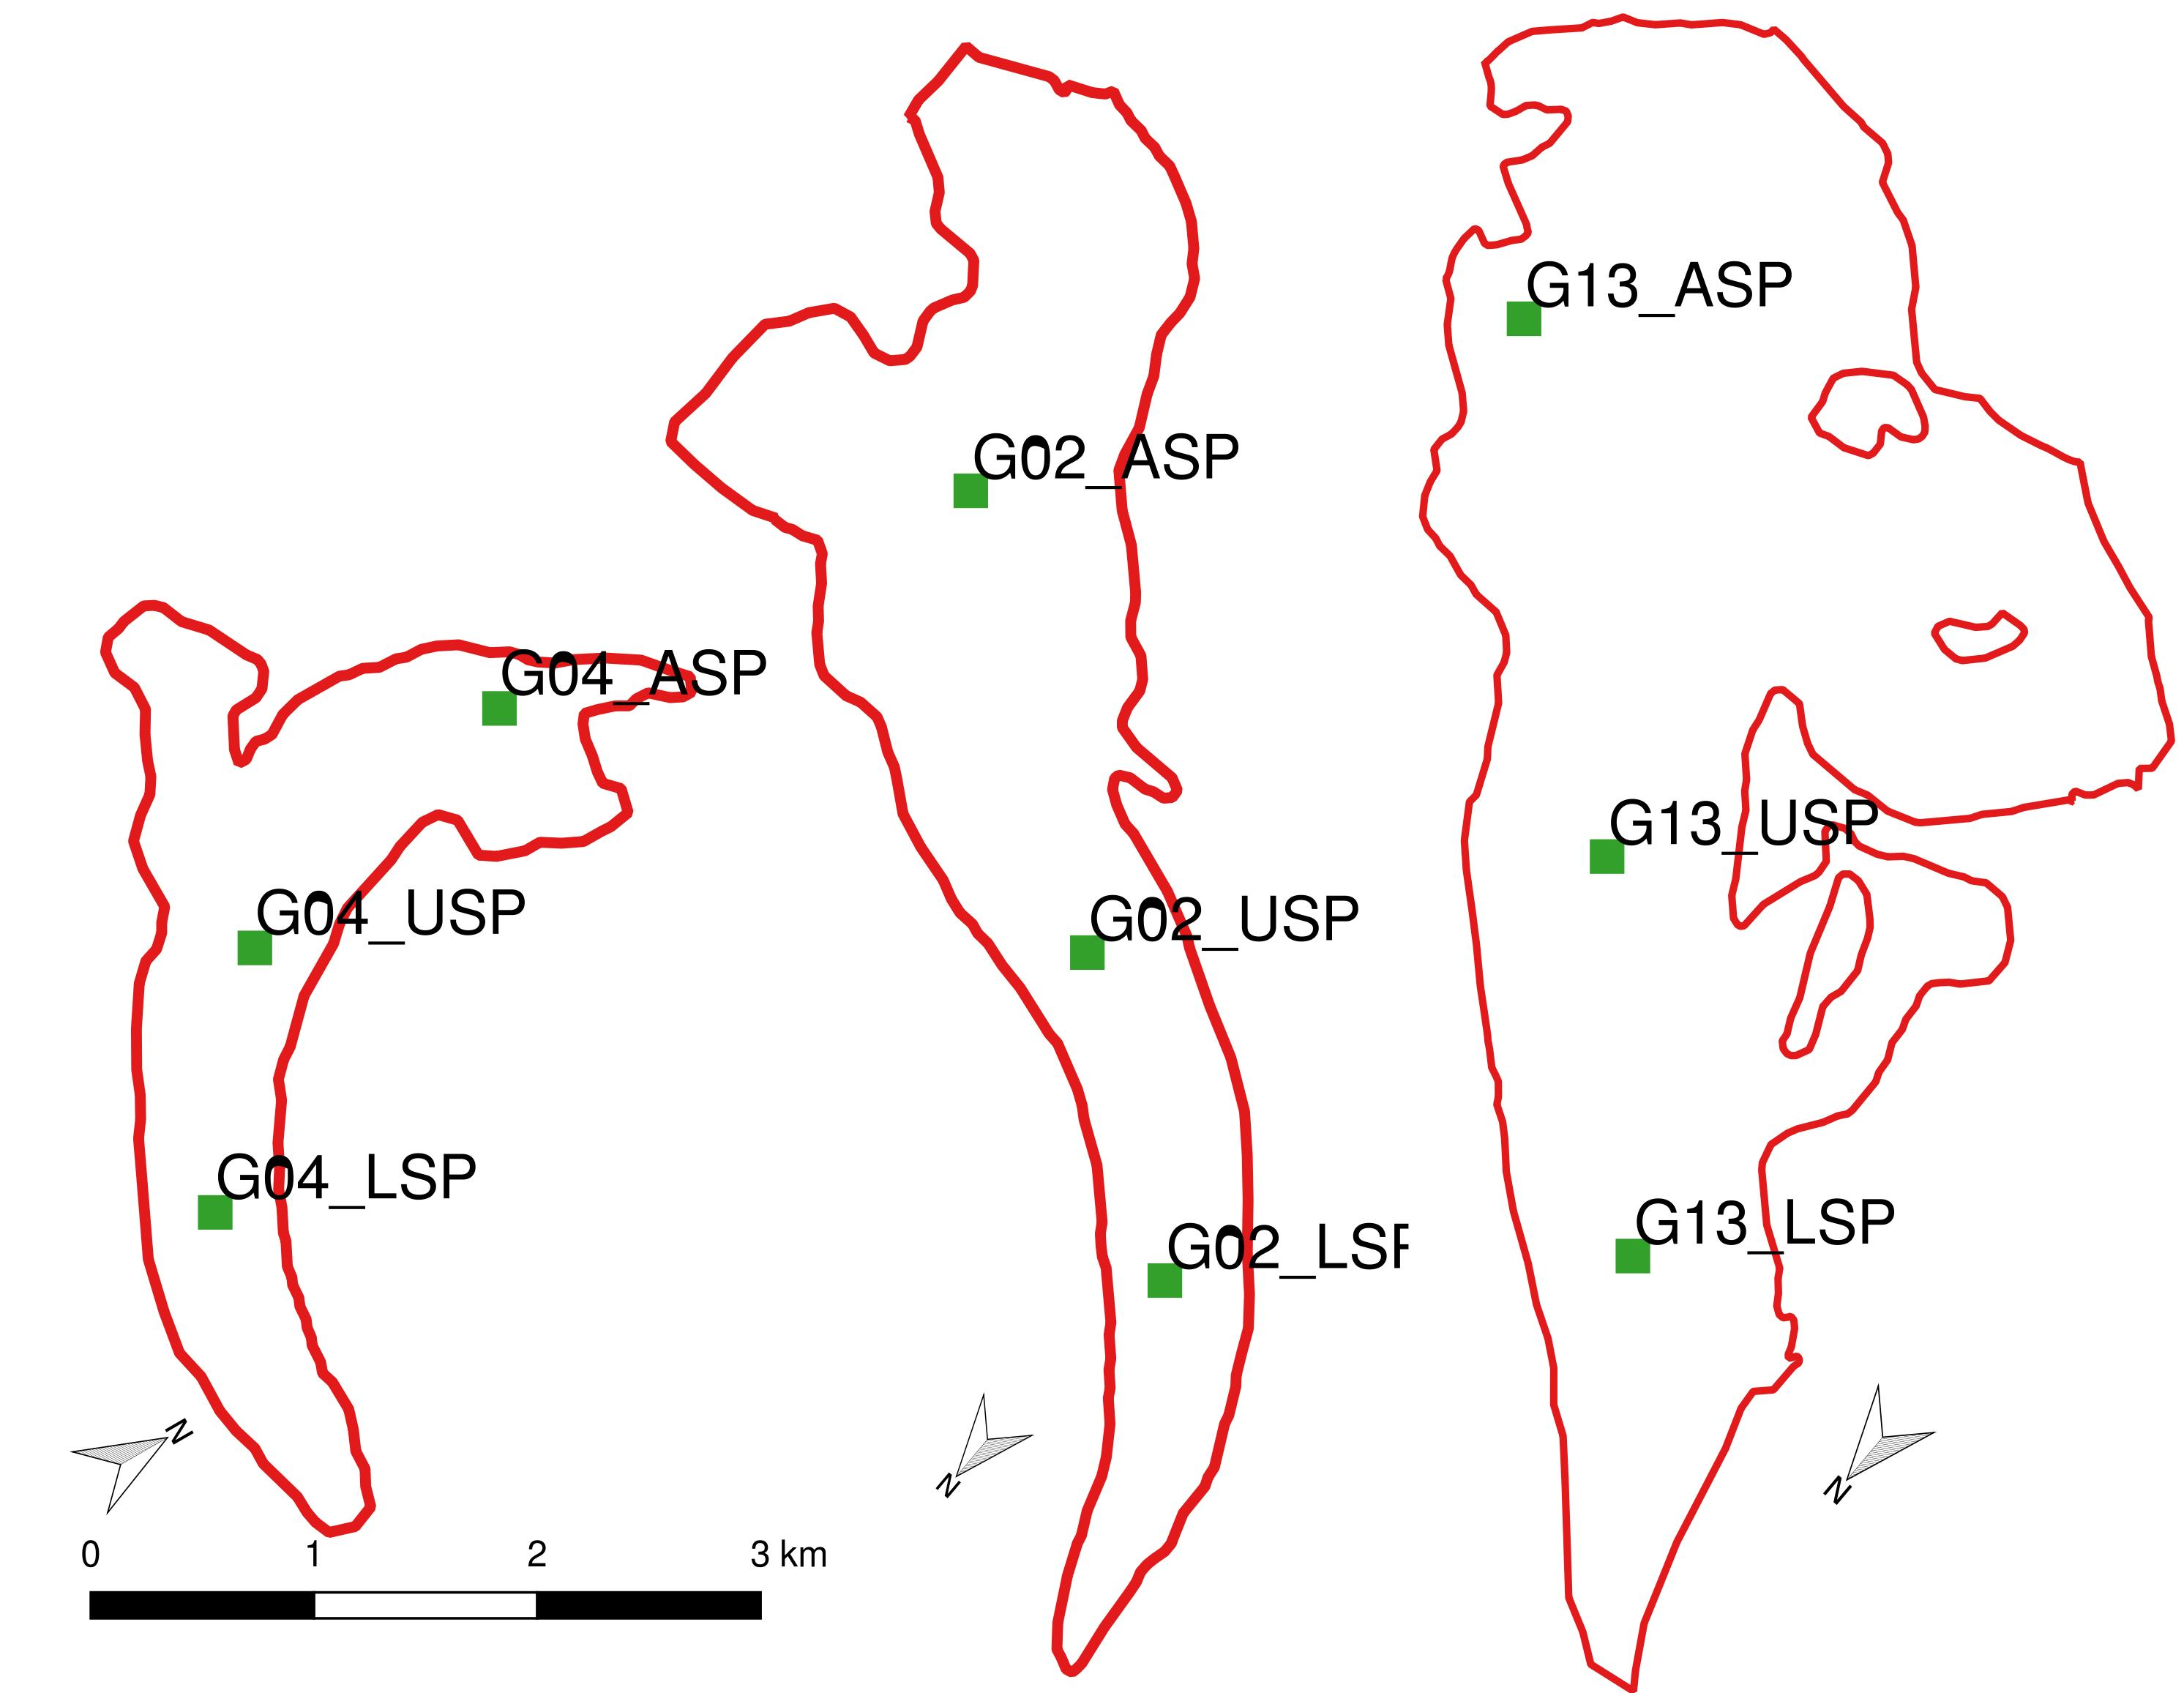
\includegraphics[width = 0.55\textwidth]{map_snowpitlocation_all.jpeg}}\\
	\caption{Locations and labels for all snowpits dug on Glaciers 4, 2 and 13 (left to right).}
	\label{fig:snowpit_location_all}
	\end{figure}

Three snowpits were excavated on each glacier (Figure \ref{fig:snowpit_location_all}) and snow density sampled every 10 cm using a wedge cutter (Snow Metrics RIP 2 Cutter (250 cc)). The snow temperature was also measured at 10 cm intervals. The snowpit was oriented so that the sampling face was in the shade (typically south edge of snowpit), which reduces melt. 

The measurement procedure in the snowpit was as follows:
\begin{enumerate}
\item The face of the wall that was chosen for sampling was smoothed and a ruler was placed against the wall with the 0 cm mark at the bottom of the snowpit. The ruler was used to measure sampling heights within the snow pack. The snow surface directly above this wall was undisturbed during the digging process so that the true snow depth could be determined. 
\item Air and snow surface temperature were measured by placing the thermometer (dial-stem thermometer ($\pm$0.5$^\circ$)) in the shade of a shovel or ski. 
\item A snow density sample was taken in 10 cm intervals through the full depth of the snow pack. Samples were offset horizontally from each other so that the snow was not affected by previous measurements. 
	\begin{enumerate}
	\item The wedge cutter was inserted into the snow vertically (to sample 10 cm intervals) and the top was slid onto the wedge to isolate the sample. The wedge was taken out and inspected. If the sample appeared to fill the entire wedge (no obvious voids) then the wedge was emptied into a small plastic bag. If the sample was poor then the snow was discarded and a new sample was taken at the same height in the snow pit. 
	\item A spring scale ($\pm$2.5 g) was then used to weigh the bag with the snow sample and the weight was recorded. The snow sample was then discarded. Note that the spring scale was tared with an empty bag.
	\end{enumerate}
\item Snow temperatures were also measured and recorded every 10 cm. The thermometer was inserted into the snow at the desired location and left to equilibrate for several minutes. The temperature was then recorded.
\end{enumerate}

Modifications to this procedure occurred when snow samples could not be taken because the snow was too dense. This would often occur when ice layers or lenses were present in the snow, which could not be cut by the wedge. In these cases, the measured thickness was recorded. A sample would then be taken using the wedge cutter but aligned horizontally so that a 5 cm tall sample was taken. Additionally, the sample interval closest to the ice surface (0--10 cm) would be difficult to obtain because the ice was rough and the snow above was faceted. Sometimes, this sample could not be obtained or a 5 cm sample needed to be taken. 

After the majority of snowpit measurements were completed, a spring scale with finer resolution was found. For Glacier 4 and 2 the coarse resolution (10 g) scale had been used but for Glacier 13 the fine resolution (2 g) scale was used. Future measurements should use the finer resolution spring scale when using the small wedge sampler. As a result, the snow-density uncertainty is larger for Glacier 4 and 2 than for Glacier 13. 

\begin{figure}
	\centering
	\fbox{\includegraphics[width = 0.95\textwidth]{photo_snowpit.jpg}}\\
	\caption{Taking snow denisty measurements in a snowpit. An expandable ruler is used to measure snow depth and determine sampling locations. A 250cc wedge cutter is used to extract a known volume of snow and a spring scale is used to weigh the snow. The dial-stem thermometer is used for measureing snow temperature. Note that the sampling wall is shaded, has an undistrubed snow surface above it, and has a smoothed face. Photo credit: A. Criscitiello}
	\label{photo_snowpit}
	\end{figure}

%%%%
\section{Data processing}
%%%%
\subsection{Snow depth measured with graduated avalanche probe}

\subsubsection{Linear and curvilinear transect surveys}

\begin{wrapfigure}{R}{0.7\textwidth}
	\centering
	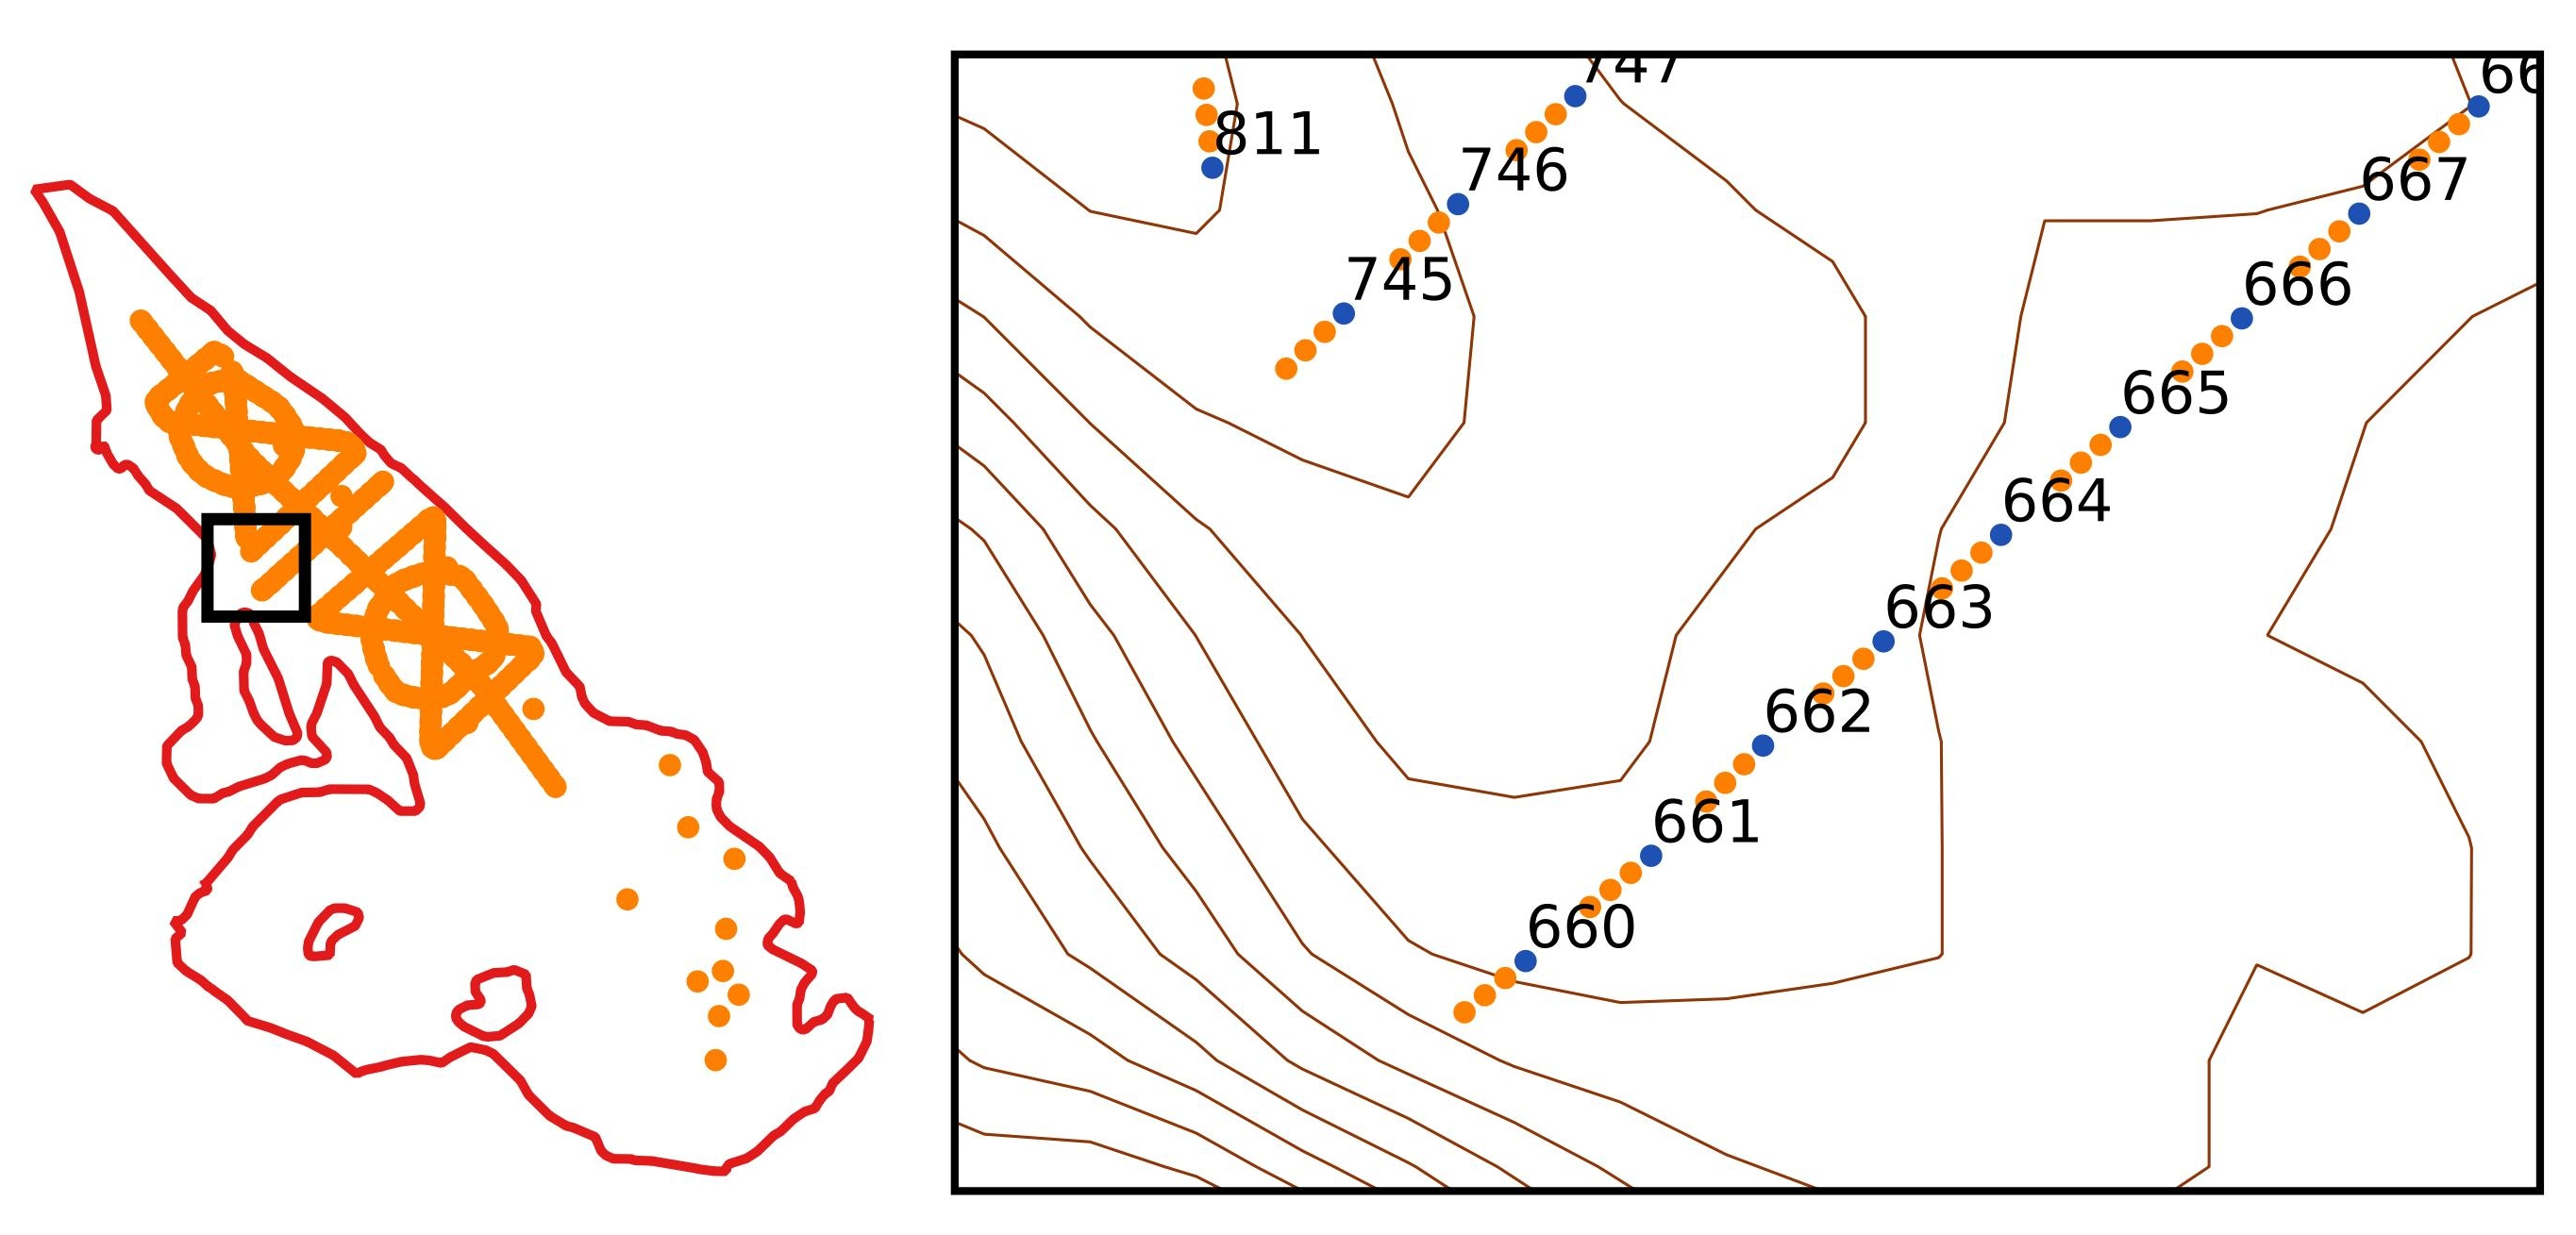
\includegraphics[width = 0.7\textwidth]{transect_measure_locations.jpeg}\\
	\caption{Example of estimating snow depth measurement locations in one area (indicted by black box) on Glacier 13. Numbered waypoint (WP) locations are shown in blue and estimated measurement locations are shown in orange at a distance of 10, 20, and 30 m from the WP. Measurement locations are taken to be along a straight line between subsequent WPs. For the first WP of a transect, the measurement locations are assumed to be along the same line as that between the first and second WPs of a transect. For example, the measurement locations behind WP 660 fall along the same line as those between WP 660 and WP 661. The same is true for WP 745. }
	\label{fig:transect_measure_loc}
\end{wrapfigure}

Snow depth measurements along the linear and curvilinear transects were taken at locations a certain distance from marked waypoints. Since only the coordinates of the waypoints (WP) were recorded, the measurement coordinates need to be estimated. The measurement locations were assumed to be 10, 20, and 30 m behind the marked WP, in a straight line between the marked WP and the previous WP (Figure \ref{fig:transect_measure_loc}). In cases with only two observers, locations were assumed to be 10 and 20 m behind the marked WP. For the first marked WP of a transect, it was assumed that the measurement locations were along the same line as that between the first and second WPs. Details of the methodology used to estimate measurement locations can be found in Appendix \ref{app:transect_calc}.

\subsubsection{Zigzag surveys}

\begin{wrapfigure}{R}{0.5\textwidth}
	\centering
	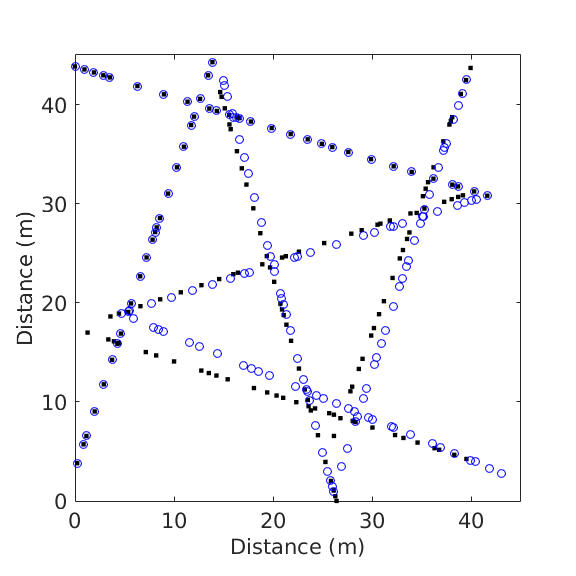
\includegraphics[width = 0.5\textwidth]{Zigzag_calOptions.png}\\
	\caption{Example of zigzag survey measurement locations calculated using difference reference vertices for each section of the zigzag. Black squares show measurement locations calculated using the original GPS coordinates of vertices (Option 1). Blue circles show measurement locations calculated using the last measurement location from the previous section as the reference vertex (Option 2). For the first and fifth vertices (located at (0, 40 m) and (0, 4 m)) the original GPS coordinates were used, which is why those sections have the same measurement locations for both options. }
	\label{fig:zigzag_location_options}
\end{wrapfigure}

Depth measurements in zigzag surveys were taken along six sections that connected eight vertices. GPS coordinates of vertices were predetermined. The survey involved navigating to the first vertex, then taking measurements at random distances from this vertex along a straight line between that vertex and the next one. The location of each measurement was measured, using the avalanche probe, and recorded as the distance from the previous measurement location. Each section was recorded separately and identified by its start, or reference, vertex. 

Originally, the location of measurements was found by taking the cumulative distance of a measurement from its reference vertex along a straight line between the reference and the next vertices. However, it was found that the cumulative distance (measured using an avalanche probe) of each zigzag section was not equivalent to the distance between UTM coordinates of each vertex (due to error in GPS and/or walking between vertices not along a straight line). Therefore, a second option for calculating the measurement locations was established. This second option still assumes the measurement was along a straight line between two vertices but the location is relative to the end of the previous section, not the reference vertex. Vertices 1 and 5 were used as reference vertices for their respective section because they began a section with no prior measurements. An example of differences between these two location estimation methods can be seen in Figure \ref{fig:zigzag_location_options}.

\subsection{Snow density}

The snowpit and Federal Sampler measurements were entered into a spreadsheet and the snow density from each measurement was calculated. For snowpit measurements the snow density was calculated by multiplying the measured density from each wedge sample by the thickness of the sample and summing these values. This is known as an integrated snow density and it encompasses the whole snow column. A density of 917 kg m$^{-3}$ was applied to ice layers and a density of 600 kg m$^{-3}$ was applied to layers that were described as `hard' and were too difficult to sample. To determine the error in estimating integrated snow density, the values of ice density, ice-layer thickness, and the `hard' layer density were varied between 700 and 917 kg m$^{-3}$, $\pm$ 1 cm (representing 20-100\% of the ice-layer thickness), and 500 and 600 kg m$^{-3}$, respectively.  A summary of density values and ranges is shown in Table \ref{tab:density_stats}.

\begin{table}[b!]
\centering
\caption{Statistics of integrated densities measured using Federal Sampler or vertical density profiles (of snow wedge measurmenets) in snow pits. Mean, standard deviation (std), and number ($n$) of snow density (kg m$^{-3}$) measurements on study glaciers is shown.}
\label{tab:density_stats}
\begin{tabular}{c|ccc|ccc}
\multirow{2}{*}{} & \multicolumn{3}{c}{\textbf{Snowpits}} & \multicolumn{3}{| c}{\textbf{Federal Sampler}} \\
 & Mean & Std & $n$ & Mean & Std & $n$ \\ \hline \hline
\textbf{Glacier 4} & 348 & 13 & 3 & 327 & 32 & 7 \\
\textbf{Glacier 2} & 333 & 26 & 4 & 326 & 23 & 7 \\
\textbf{Glacier 13} & 349 & 26 & 10 & 307 & 32 & 31 \\ \hline
\textbf{All} & 342 & 26 & 10 & 316 & 31 & 31
\end{tabular}
\end{table}

Density values determined from Federal Sampler measurements that were deemed to be unrepresentative of the local snow pack, including measurements where the inner core length was less than 70\% of the snow depth or where density values were exceptionally high (e.g. 490 kg m$^{-3}$), were flagged as poor quality and removed. The remaining Federal Sampler density values were then averaged for each measurement location.

\subsection{Snow water equivalent (SWE)}
\label{sec:swe_calc}

\begin{wrapfigure}{R}{0.7\textwidth} 
	\centering
	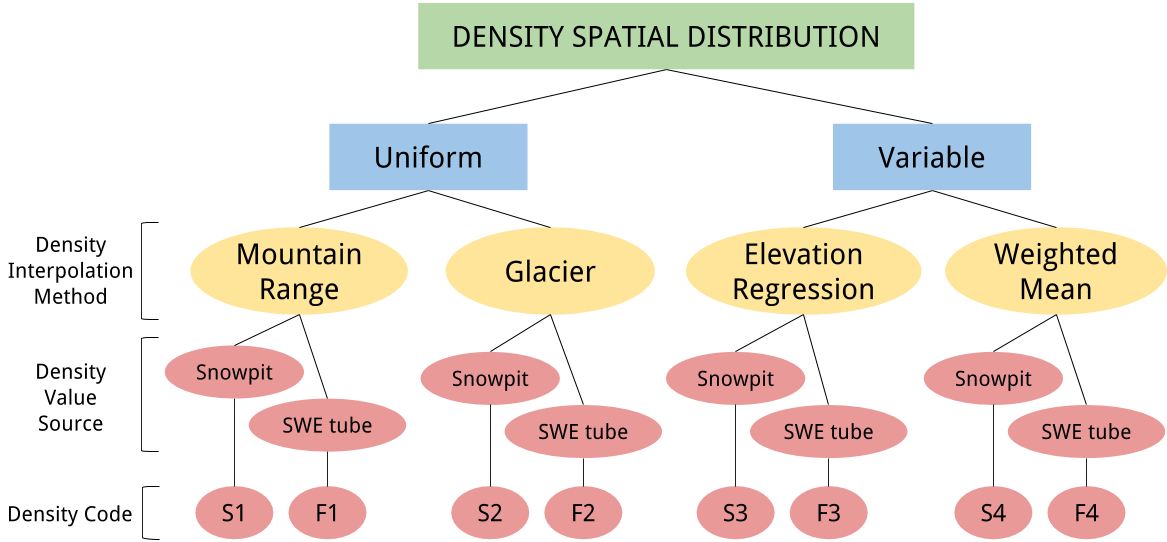
\includegraphics[width = 0.7\textwidth]{SWEoptions.png}\\
	\caption{Relationship between various ways to interpolate between density measurements for the calculation of SWE. The bottom row shows the code for each density interpolation option as described in Section \ref{sec:swe_calc}.}
	\label{fig:SWEoptions}
\end{wrapfigure}

The conversion of measured snow depth to snow water equivalent (SWE) could not be done at all measurement locations because snow density was not measured at all locations where snow depth was measured. This meant that the density measurements need to be interpolated. A subset of appropriate interpolation methods was chosen for this project. In the absence of a clear justification for choosing one option over the other, all options were carried forward in the analysis. A schematic of the interpolation method choices is shown in Figure \ref{fig:SWEoptions}. 

Four main interpolation methods are used \citep{McGrath2015, Elder1991}. The first assumes a uniform spatial distribution of density, calculated as the mean from all measurement locations on all three glaciers, over the entire study area. The second  also assumes a uniform spatial distribution of density but uses a mean density for individual glaciers (different value for each glacier). The third and fourth methods involve spatially variable density values. One of these methods involves using a regression of elevation and measured density values to interpolate between measurement locations. The other spatially variable interpolation method uses an inverse-distance weighted mean for interpolation. 

Since the snowpit-derived densities and Federal Sampler-derived densities had no discernible relationship, the two density datasets are kept separate. This means that for each density interpolation option, there are two outputs. In the end, there are eight different interpolations of density that are carried forward throughout the study, which allows for a range of SWE estimates to be made. 

The eight density distributions can be classified as using either snowpit-derived densities (SP) or Federal Sampler-derived densities (FS) and as using a certain method, indicated by a number.
\begin{itemize}
	\item[S1] Calculates the mean density of all snowpit measurements.
	\item[F1] Calculates the mean density of all Federal Sampler measurements.
	\item[S2] Calculates the mean density for each glacier using the snowpit measurements. 
	\item[F2] Calculates the mean density for each glacier using the Federal Sampler measurements. 
	\item[S3] Calculates the slope and intercept of the best-fit regression line of snowpit densities with elevation for each glacier using the `fit' function and then uses slope and intercept to determine density for all elevations associated with each measurement location.
	\item[F3] Calculates the slope and intercept of the best-fit regression line of Federal Sampler densities with elevation for each glacier using the `fit' function and then uses the slope and intercept to determine density for all elevations associated with each measurement location.
	\item[S4] Determines the distance between each measurement location and each snowpit and then calculates the inverse-distance weight. For each measurement location, each snowpit density is then multiplied by its weight and these values are added together and divided by the sum of all weights. 
	\item[F4] Determines the distance between each measurement location and each Federal Sampler and then calculates the inverse-distance weight. For each measurement location, each Federal Sampler density is then multiplied by its weight and these values are added together and divided by the sum of all weights. 
	\end{itemize}



\chapter{Data observations}

%%%
\section{Density Estimates}
%%%
\label{sec:density}

\subsection{Basic statistics}

The standard deviation of each type of density measurement is less than 10\% of the mean density (Table \ref{tab:density_stats}). For snowpit derived densities, the mean density is within one standard deviation between glaciers . The densities estimated using the Federal Sampler differed between glacier within one standard deviation. Our density measurements on Glacier 2 were lower than those on Glacier 4, while density measurements taken on Glacier 13 were the same as Both Glaciers 2 and 4. The mean of all Federal Sampler derived density values was skewed by the proportionally large number of measurements obtained on Glacier 13.

\subsection{Federal Sampler measurements and snow depth}
\label{sec:FSdensity&depth}

There is a positive linear relation (R$^2$ = 0.59, p$<$0.01) between measured snow density and depth for all Federal Sampler measurements (Figure \ref{fig:all_depth}). This positive relationship could be a result of physical processes, such as compaction, and/or artefacts during data collection; however, it seems more likely that this trend is a result of measurement artefacts for a number of reasons. First, the range of densities measured by the Federal sampler is large (225--410 kg m$^{-3}$) and the extreme values seem unlikely to exist at these study glaciers, which experience a continental snowpack with minimal mid-winter melt events. Previous unpublished density measurements taken on Glacier 2 for five study years have a mean snow density of 298 kg m$^{-3}$ and a standard deviation of 48 kg m$^{-3}$ (range of 264-396 kg m$^{-3}$ with a maximum density difference of 110 kg m$^{-3}$ in any one year) (Flowers, 2016, personal communication). Second, compaction effects would likely be small at these study glaciers because of the relatively shallow snowpack (deepest measurement was 340 cm). Third, no linear relationship exists between depth and snowpit-derived density (R$^2$ = 0.05) as can be seen in a plot of the depth-density relationship in snowpits in Figure \ref{fig:all_depth}. Together, these reasons lead us to conclude that the Federal Sampler measurements are biased. Linear detrending can correct the density data but it was decided to use uncorrected data for future analysis.

The Federal Sampler appears to oversample in deep snow and undersample in shallow snow. Oversampling by small diameter (area of 1O--12 cm$^2$) sampling tubes has been observed in previous studies, with a percent error between +6.8\% and 11.8\%\citep{Work1965, Fames1982, Conger2009}. Studies that use Federal Samplers often apply a 10\% correction to all measurements \citep[e.g.][]{Molotch2005}. \cite{Dixon2012} attributed oversampling to slots ``shaving'' snow into the tube as it is rotated as well as cutter deign forcing snow into the tube. \cite{Beaumont1963} found that only when snow samples had densities greater than 400 kg m$^{-3}$ and snow depth greater than 1 m, the Federal Sampler oversampled due to snow falling into the greater area of slots. Undersampling is likely to occur due to snow falling out of the bottom of the sampler \citep{Turcan1975}. It is likely that this occurred during our study since a large portion of the lower elevation snow on both Glaciers 2 and 13 was melt affected and thin, allowing for easier lateral displacement of the snow as the sampler was inserted. For example, on Glacier 13 the snow surface had been affected by radiation melt (especially at lower elevations where the snow was shallower) and the surface would collapse when the sampler was inserted into the snow. It is also difficult to measure the weight of the sampler and snow with the spring scale when there was little snow because the weight was at the lower limit of what could be detected by the scale. 



\begin{figure}[p]
	\centering
	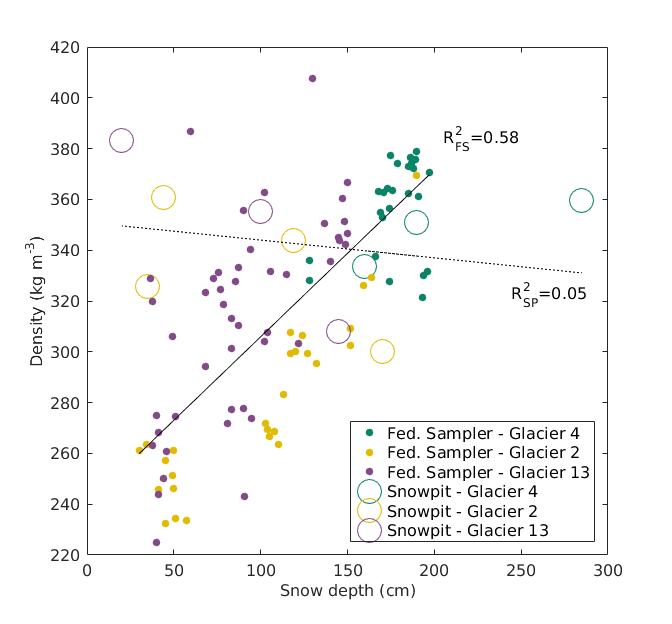
\includegraphics[width =0.85\textwidth]{DepthDensity_SWEonly.png}\\
	\caption{Relationship between measured density and snow depth for all Federal Sampler and snowpit locations. A linear regression of depth and density for Federal Sampler (FS) measurements is shown as a solid line and for snowpits (SP) is shown as a dashed line.}
	\label{fig:all_depth}
\end{figure}


\subsection{Density uncertainties}

\subsubsection{Snowpit densities}

Uncertainty in estimating density from snowpits stems from measurement errors and incorrect assignment of density to layers that could not be sampled (i.e. ice lenses and `hard' layers). To determine a possible range of snowpit-derived integrated snow density values, the original data are used and three quantities are varied. Ice layer density is varied between 700 and 900 kg m$^{-3}$, ice layer thickness is varied by $\pm$1 cm of the observed thickness, and the density of layers identified as being too hard to sample (but not ice) was varied between 600 and 700 kg m$^{-3}$. 

The range of integrated density values is always less than 15\% of the reference density, with the largest ranges present on Glacier 2 (Table \ref{tab:density_SP}). Density values for shallow pits that contained ice lenses were particularly sensitive to changes in density and ice lens thickness. 

\begin{sidewaystable}[]
\centering
\caption{Summary of reference and range of integrated snow density calculated from  snowpit measurements. The reference density values are calculated with an ice layer density of 917 kg m$^{-3}$ and a `hard' snow density of 600 kg m$^{-3}$. To determine the error in estimating integrated snow density, ice density, ice thickness, and the `hard' layer density are varied between 700 and 917 kg m$^{-3}$, $\pm$ 1 cm, and 500 and 600 kg m$^{-3}$, respectively.}
\label{tab:density_SP}
\resizebox{\textwidth}{!}{%
\begin{tabular}{lcccccccc}
\multirow{2}{*}{\textbf{Snowpit Name}} &  & \multicolumn{4}{c}{\textbf{Density (kg m$^{-3}$)}} &  \\
\multirow{-2}{*}{} & \multirow{-2}{*}{\textbf{Depth (m)}} & \textit{Reference} & \textit{Minimum} & \textit{Maximum} & \textit{Range} & \multirow{-2}{*}{\textbf{\begin{tabular}[c]{@{}c@{}}Range as \% \\ of reference value\end{tabular}}} & \multirow{-2}{*}{\textbf{\begin{tabular}[c]{@{}c@{}}Elevation\\ (m a.s.l)\end{tabular}}}& \multirow{-2}{*}{\textbf{\begin{tabular}[c]{@{}c@{}}Average \\ Temperature ($^{\circ}$) \end{tabular}}}\\ \hline \hline

Glacier 4, Lower & 190 & 350.9 & 343.2 & 359.1 & 15.9 & 4.5 & 2154 & $-$ 4.3\\
Glacier 4, Upper & 160 & 333.4 & 316.6 & 349.6 & 33.0 & 9.9  & 2298 & $-$ 5.7\\
Glacier 4, Accumulation& 285 & 359.7 & 356.6 & 362.4 & 5.8 & 1.6  & 2482 & $-$ 6.8\\  \hline
Glacier 2, Lower  & 44 & 360.9 & 328.6 & 377.3 & 48.7 & 13.5 & 2175 & $-$ 3.7 \\
Glacier 2, Zone 4A & 35 & 325.8 & 307.9 & 344.7 & 36.8 & 11.3 & 2261 & $-$ 3.4 \\
Glacier 2, Upper  & 119 & 344.0 & 327.1 & 361.9 & 34.8 & 10.1 & 2349 & $-$ 6.6 \\ 
Glacier 2, Accumulation & 170 & 300.2 & 298.6 & 303.1 & 4.5 & 1.5  & 2550 & $-$ 7.4\\  \hline
Glacier 13, Lower  & 20 & 383.0 & 383.0 & 383.0 & 0 & 0  & 2139 & $-$ 0.1\\
Glacier 13, Upper & 100 & 355.4 & 345.6 & 366.9 & 21.3 & 6.0 & 2257 & $-$ 1.7 \\
Glacier 13, Accumulation & 145 & 307.8 & 306.4 & 308.2 & 1.8 & 0.6 & 2521 & $-$ 5.6
\end{tabular}%
}
\end{sidewaystable}

\subsubsection{Federal Sampler densities}

Mean Federal Sampler derived density has a larger range of values over the study glaciers when compared to snowpit densities (Table \ref{tab:density_TubeRange}). The percent range is also larger than snowpit densities for many of the measurement locations. 

\begin{table}[]
\centering
\caption{Range of densities estimated from Federal Sampler measurements. The number ($n$) of reliable measurements, as well as the minimum, maximum, and mean density are shown. The density range, given as a percent of the mean density, is also shown. Location refers to the snowpit name as shown in Figure \ref{fig:snowpit_location_all}.}
\label{tab:density_TubeRange}
\begin{tabular}{lcccccc}
\multicolumn{1}{c}{\multirow{2}{*}{\textbf{Location}}} & \multirow{2}{*}{\textbf{$n$}} & \multicolumn{3}{c}{\textbf{Density (kg m$^{-3}$)}} & \multirow{2}{*}{\textbf{\begin{tabular}[c]{@{}c@{}}Range as \%\\ of mean (\%)\end{tabular}}}& \multirow{2}{*}{\textbf{\begin{tabular}[c]{@{}c@{}}Elevation\\ (m a.s.l)\end{tabular}}} \\
\multicolumn{1}{c}{} &  & Mean & Minimum & Maximum &  \\ \hline  \hline
G04\_Z3A\_SWE & 3 & 334 & 309 & 358 & 14 & 2229 \\
G04\_USP & 6 & 311 & 274 & 353 & 22 & 2298 \\
G04\_Z2A\_SWE & 3 & 360 & 303 & 431 & 35 & 2162 \\
G04\_LSP & 7 & 272 & 250 & 297 & 13 & 2154 \\
G04\_Z5B\_SWE & 2 & 337 & 324 & 350 & 7  & 2360\\
G04\_Z5A\_SWE & 3 & 311 & 275 & 351 & 21  & 2328\\
G04\_Z5C\_SWE & 2 & 361 & 350 & 373 & 6  & 2332\\  \hline
G02\_Z5C\_SWE & 2 & 296 & 245 & 347 & 28 & 2332 \\
G02\_USP & 7 & 294 & 232 & 353 & 34  & 2349\\
G02\_Z7A\_SWE & 3 & 326 & 304 & 349 & 12  & 2403\\
G02\_Z7B\_SWE & 2 & 336 & 320 & 351 & 9 & 2458 \\
G02\_Z7C\_SWE & 3 & 351 & 338 & 365 & 7 & 2442 \\
G02\_Z3B\_SWE & 3 & 349 & 341 & 353 & 3  & 2172\\
G02\_LSP\_SWE & 7 & 331 & 302 & 349 & 13 & 2175 \\ \hline
G13\_ASP & 8 & 343 & 277 & 395 & 33  & 2521\\
G13\_651 & 3 & 329 & 318 & 345 & 7  & 2574\\
G13\_652 & 2 & 319 & 291 & 346 & 15  & 2542\\
G13\_654 & 3 & 298 & 266 & 318 & 14  & 2571\\
G13\_655 & 1 & 300 &-- & -- & --  & 2561\\
G13\_656 & 3 & 279 & 227 & 315 & 24  & 2541\\
G13\_657 & 3 & 331 & 323 & 338 & 4  & 2483\\
G13\_658 & 2 & 343 & 333 & 354 & 6  & 2427\\
G13\_659 & 3 & 245 & 232 & 258 & 7 & 2327 \\
G13\_Z7C\_SWE & 2 & 270 & 253 & 287 & 9  & 2297\\
G13\_USP & 6 & 294 & 247 & 359 & 31  & 2258\\
G13\_Z4C\_SWE & 4 & 342 & 334 & 350 & 5 & 2206 \\
G13\_744 & 3 & 323 & 298 & 347 & 14 & 2210 \\
G13\_Z3B\_SWE & 3 & 333 & 308 & 351 & 12 & 2156 \\
G13\_Z4B\_SWE & 2 & 332 & 312 & 351 & 11  & 2214\\
G13\_Z5A\_SWE & 3 & 276 & 240 & 301 & 17  & 2271\\
G13\_Z5B\_SWE & 2 & 255 & 254 & 257 & 1 & 2226
\end{tabular}
\end{table}

\subsection{Comparing density from snowpit and Federal Sampler measurements}

To compare snowpit-derived densities and Federal Sampler-derived densities, eight Federal Sampler measurements were taken around two snowpit locations on each study glacier.  The overall range of Federal Sampler-derived densities is larger than that of the snowpit-derived density values (Figure \ref{fig:density_pitVStube}). Within the minimum and maximum snowpit-derived densities, the values are indistinguishable for all snowpit locations, except for the accumulation snowpit on Galcier 13 (`G13\_ASP').

\begin{figure}[H]
	\centering
	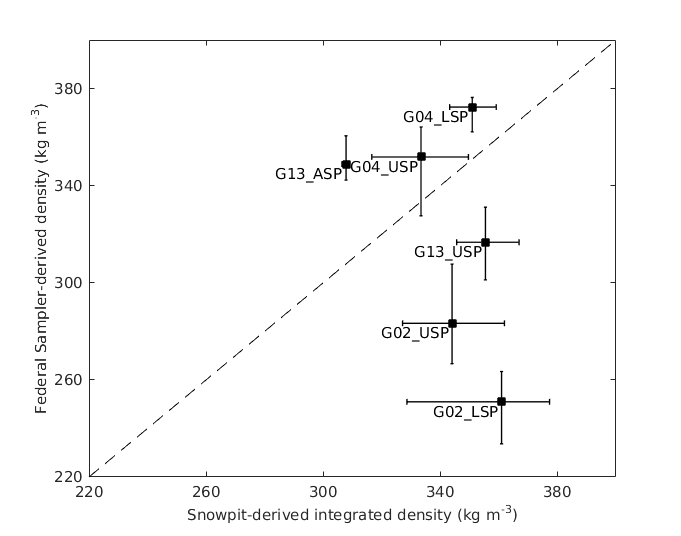
\includegraphics[width =0.95\textwidth]{SnowpitVsSWEtube_all.png}\\
	\caption{Comparison of integrated density estimated using wedge cutters in a snowpit and density estimated using Federal Sampler measurements for Glacier 4 (G04), Glacier 2 (G02) and Glacier 13 (G13). Error bars are minimum and maximum values for each estimate as reported in Table \ref{tab:density_SP} and \ref{tab:density_TubeRange}. }
	\label{fig:density_pitVStube}
\end{figure}


\subsection{Density and elevation}

A linear regression of density on topographic parameters is often used to interpolate density values between measurement locations \citep[e.g.][]{Elder1998, Molotch2005,Wetlaufer2016}. Since the density measurement locations spanned a large portion of the elevation range for each glacier, the density values are regressed on elevation only. Regression slopes differ in both magnitude and sign between snowpit-derived and Federal Sampler-derived densities (Table \ref{tab:elev_regress}). 

Snowpit-derived density decreases with elevation on Glaciers 2 and 13 and does not change with elevation on Glacier 4 (Figure \ref{fig:elev_snowpit}). The lower elevation sites on Glaciers 2 and 13 could have been melt affected. Warmer mean snow temperatures at the lower sites (Table \ref{tab:density_SP}) indicate that melt has occurred, which would increase snow density. Glacier 4 was probably not affect by melt, as snow temperatures are cool at all snowpit sites. 

Opposite relationship are seen in the regression of Federal Sampler-derived densities and elevation (Figure \ref{fig:elev_tube}). Density increases with elevation on Glacier 2 and there is no relationship with elevation on Glacier 4 and 13. The is a positive relationship between snow density and snow depth (Section \ref{sec:FSdensity&depth}) and a positive relationship between snow depth and elevation (Figure \ref{fig:depth_elev}) on Glacier 2, which results in a positive relationship between snow density and elevation. Since there is no significant relationship between snow depth and elevation on Glaciers 4 and 13, there is no relationship between snow density and elevation. 


\begin{table}[]
\centering
\caption{Summary of linear regressions between integrated density and elevation (m a.s.l.). }
\label{tab:elev_regress}
\begin{tabular}{lrrcrcc}
\multicolumn{1}{c}{\multirow{2}{*}{\textbf{Location}}} & \multicolumn{3}{c}{\textbf{\begin{tabular}[c]{@{}c@{}}Snowpit \\ Regression\end{tabular}}} & \multicolumn{3}{c}{\textbf{\begin{tabular}[c]{@{}c@{}}Fed. Sampler\\ Regression\end{tabular}}} \\
\multicolumn{1}{c}{} & \multicolumn{1}{c}{Equation} & \multicolumn{1}{c}{R$^2$} & \multicolumn{1}{l}{$n$} & \multicolumn{1}{c}{Equation} & R$^2$ & \multicolumn{1}{l}{$n$} \\ \hline \hline
Glacier 4 & 0.03$z+$274 & 0.16 & 3 & $-$0.16$z+$714 & 0.53 & 7 \\
Glacier 2 & $-$0.14$z+$659 & 0.75 & 4 & 0.24$z-$282 & 0.72 & 7 \\
Glacier 13 & $-$0.20$z+$802 & $>$0.99 & 3 & 0.12$z+$33 & 0.21 & 17 \\ \hline
All & $-$0.12$z+$618 & 0.50 & 10 & $-$0.14$z+$659 & 0.75 & 31
\end{tabular}
\end{table}


\begin{figure}[H]
  \makebox[\textwidth][c]{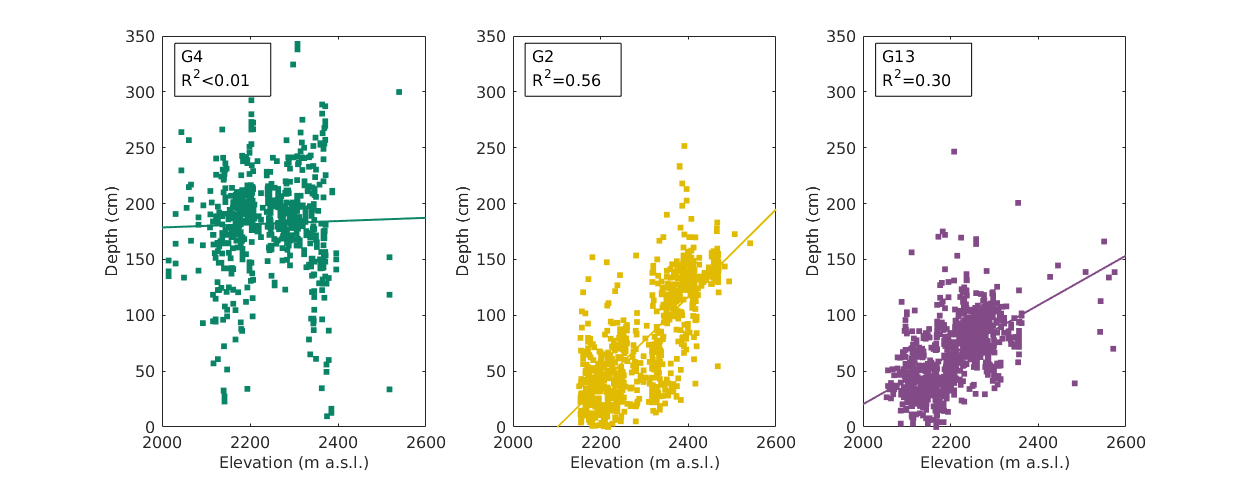
\includegraphics[width=1.2\textwidth]{DepthElevation.png}}%
	\caption{Relationship between measured snow depth and elevation at all sampling locations.}
	\label{fig:depth_elev}
\end{figure}


\begin{figure}[H]
	\centering
	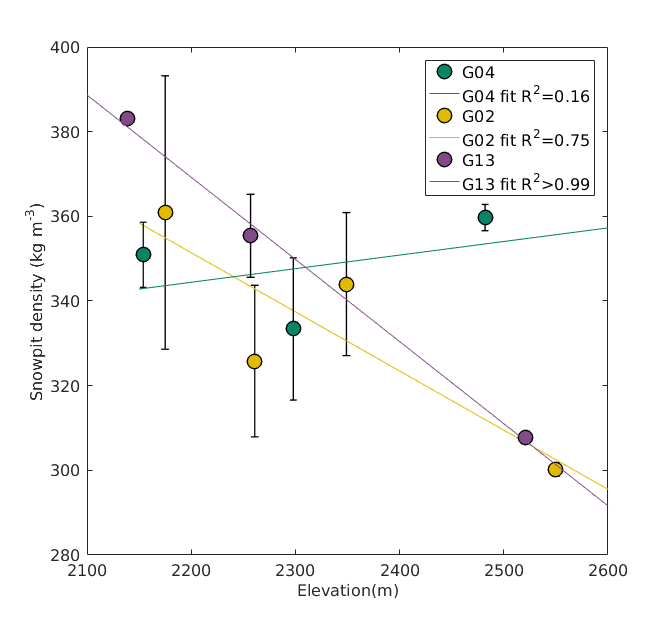
\includegraphics[width = 0.6\textwidth]{ElevationVsSnowpit_all.png}\\
	\caption{Relationship between snowpit-derived density and elevation for all study glaciers.}
	\label{fig:elev_snowpit}
\end{figure}


\begin{figure}[H]
	\centering
	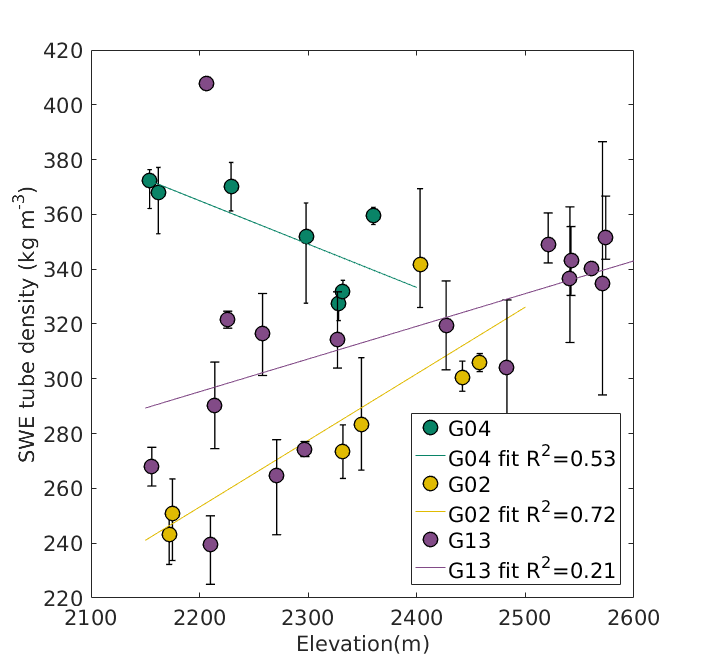
\includegraphics[width = 0.5\textwidth]{ElevationVsSWEtube_all.png}\\
	\caption{Relationship between Federal Sampler-derived density and elevation for all study glaciers.}
	\label{fig:elev_tube}
\end{figure}


\pagebreak

%%%%%%%%%%%%%%%%%%%%%%%%%%%%%%%%%%%%%%
\section{Linear and curvilinear transect snow depth data}

\begin{figure}[H]
    \centering
    \begin{subfigure}[b]{0.48\textwidth}
        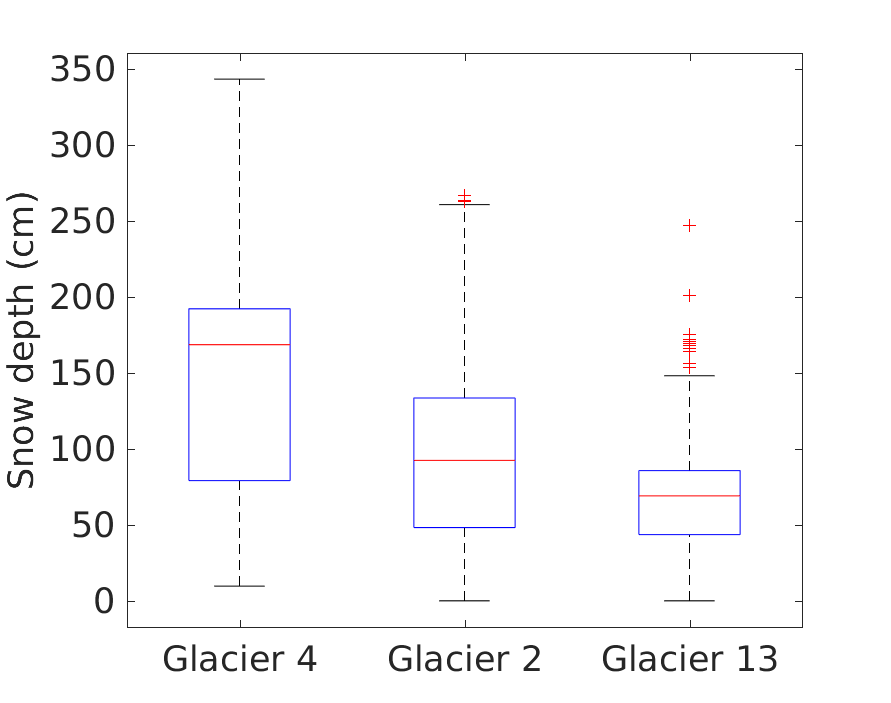
\includegraphics[width=\textwidth]{box_depth_wZZ.png}
        \caption{ }
        \label{fig:box_depth_wZZ}
    \end{subfigure}
    ~
    \begin{subfigure}[b]{0.48\textwidth}
        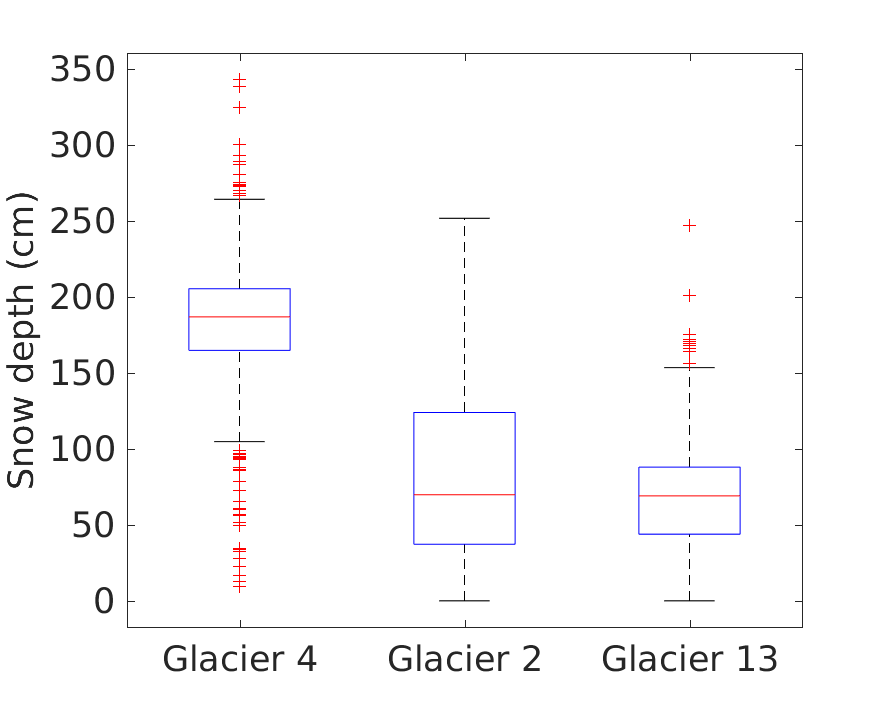
\includegraphics[width=\textwidth]{box_depth_noZZ.png}
        \caption{}
        \label{fig:box_depth_noZZ}
    \end{subfigure}

    \caption{Boxplots of snow depth measured on study glaciers. All snow depth values shown in (a) and snow depth values only from transects (zigzag, snowpit and Federal Sampler measurements excluded) shown in (b). Red line indicates median, blue box shows first quantiles, bars indicate minimum and maximum values (excluding outliers), and red crosses show outliers, which are defined as being outside of the range of 1.5 times the quartiles (approximately $\pm2.7\sigma$).}
    \label{fig:box_depth}
\end{figure}

Glacier 4 has the largest median and range of snow depth values, while Glacier 13 has the smallest (Figure \ref{fig:box_depth}). The boxplot of snow depth on Glacier 4 has different characteristics when only transect data is plotted (zigzag, snowpit and Federal Sampler measurements excluded). The range and IQR are smaller and there are significantly more points that are considered outliers. 

\pagebreak
%%%%%%%%%%%%%%%%%%%%%%%%%%%%%%%%%%%%%%
\section{Zigzag snow depth data}

A comparison of measured snow depth for each zigzag is shown in Figure \ref{fig:ZZ_boxplot}. The zigzags on Glacier 4 show minimal variability with a small range of values observed and few outliers. The mean depth is significantly larger at the highest elevation zigzag. Zigzags on Glacier 2 show more variability. The range on the middle elevation is the largest of all the zigzags measured and the highest zigzag has many outliers. The zigzags on Glacier 13 do not vary considerably in range, although the lower zigzags show a large number of outliers which may be a result of these locations being close to a supraglacial meltwater channel. 

The depths measured in each zigzag are shown in Figures \ref{fig:ZZ_G04}, \ref{fig:ZZ_G02}, and \ref{fig:ZZ_G13}. There is considerable variability both between zigzags and within each zigzag. For example, snow depths in G04\_Z5B are more uniform than in G04\_Z3A (Figure \ref{fig:ZZ_G04}). 

\begin{figure}[H]
	\centering
	 \makebox[\textwidth][c]{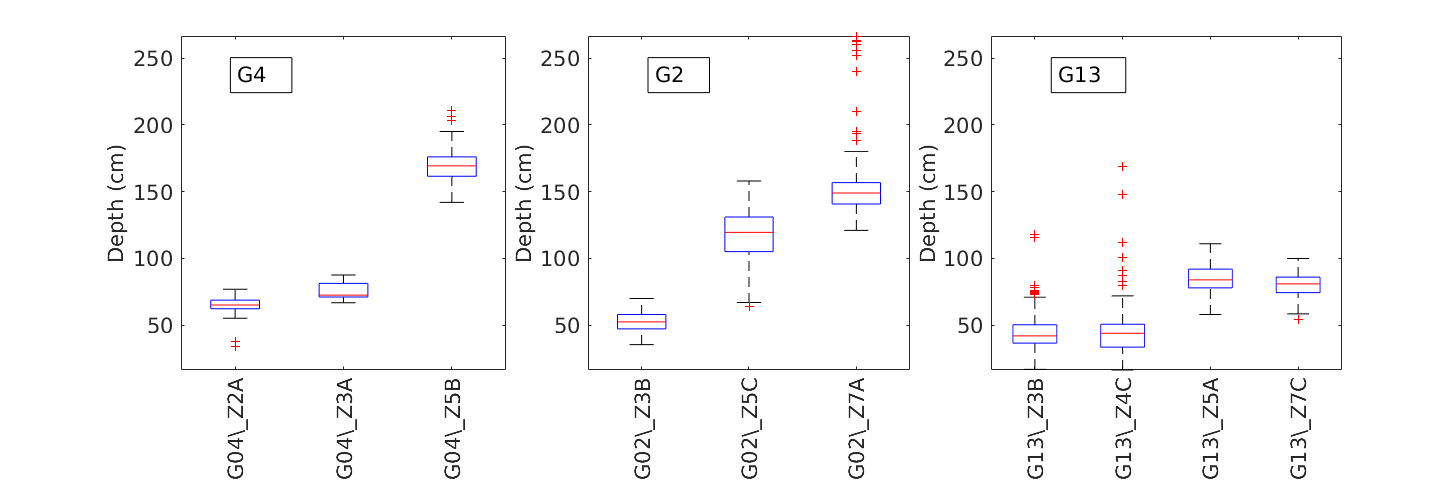
\includegraphics[width = 1.1\textwidth]{Zigzag_Boxplot.png}}%
	\caption{Boxplots of snow depth data measured at each zigzag location. See Figure \ref{fig:ZZ_locations} for locations of each zigzag.}
	\label{fig:ZZ_boxplot}
\end{figure}


\begin{figure}[H]
	\centering
	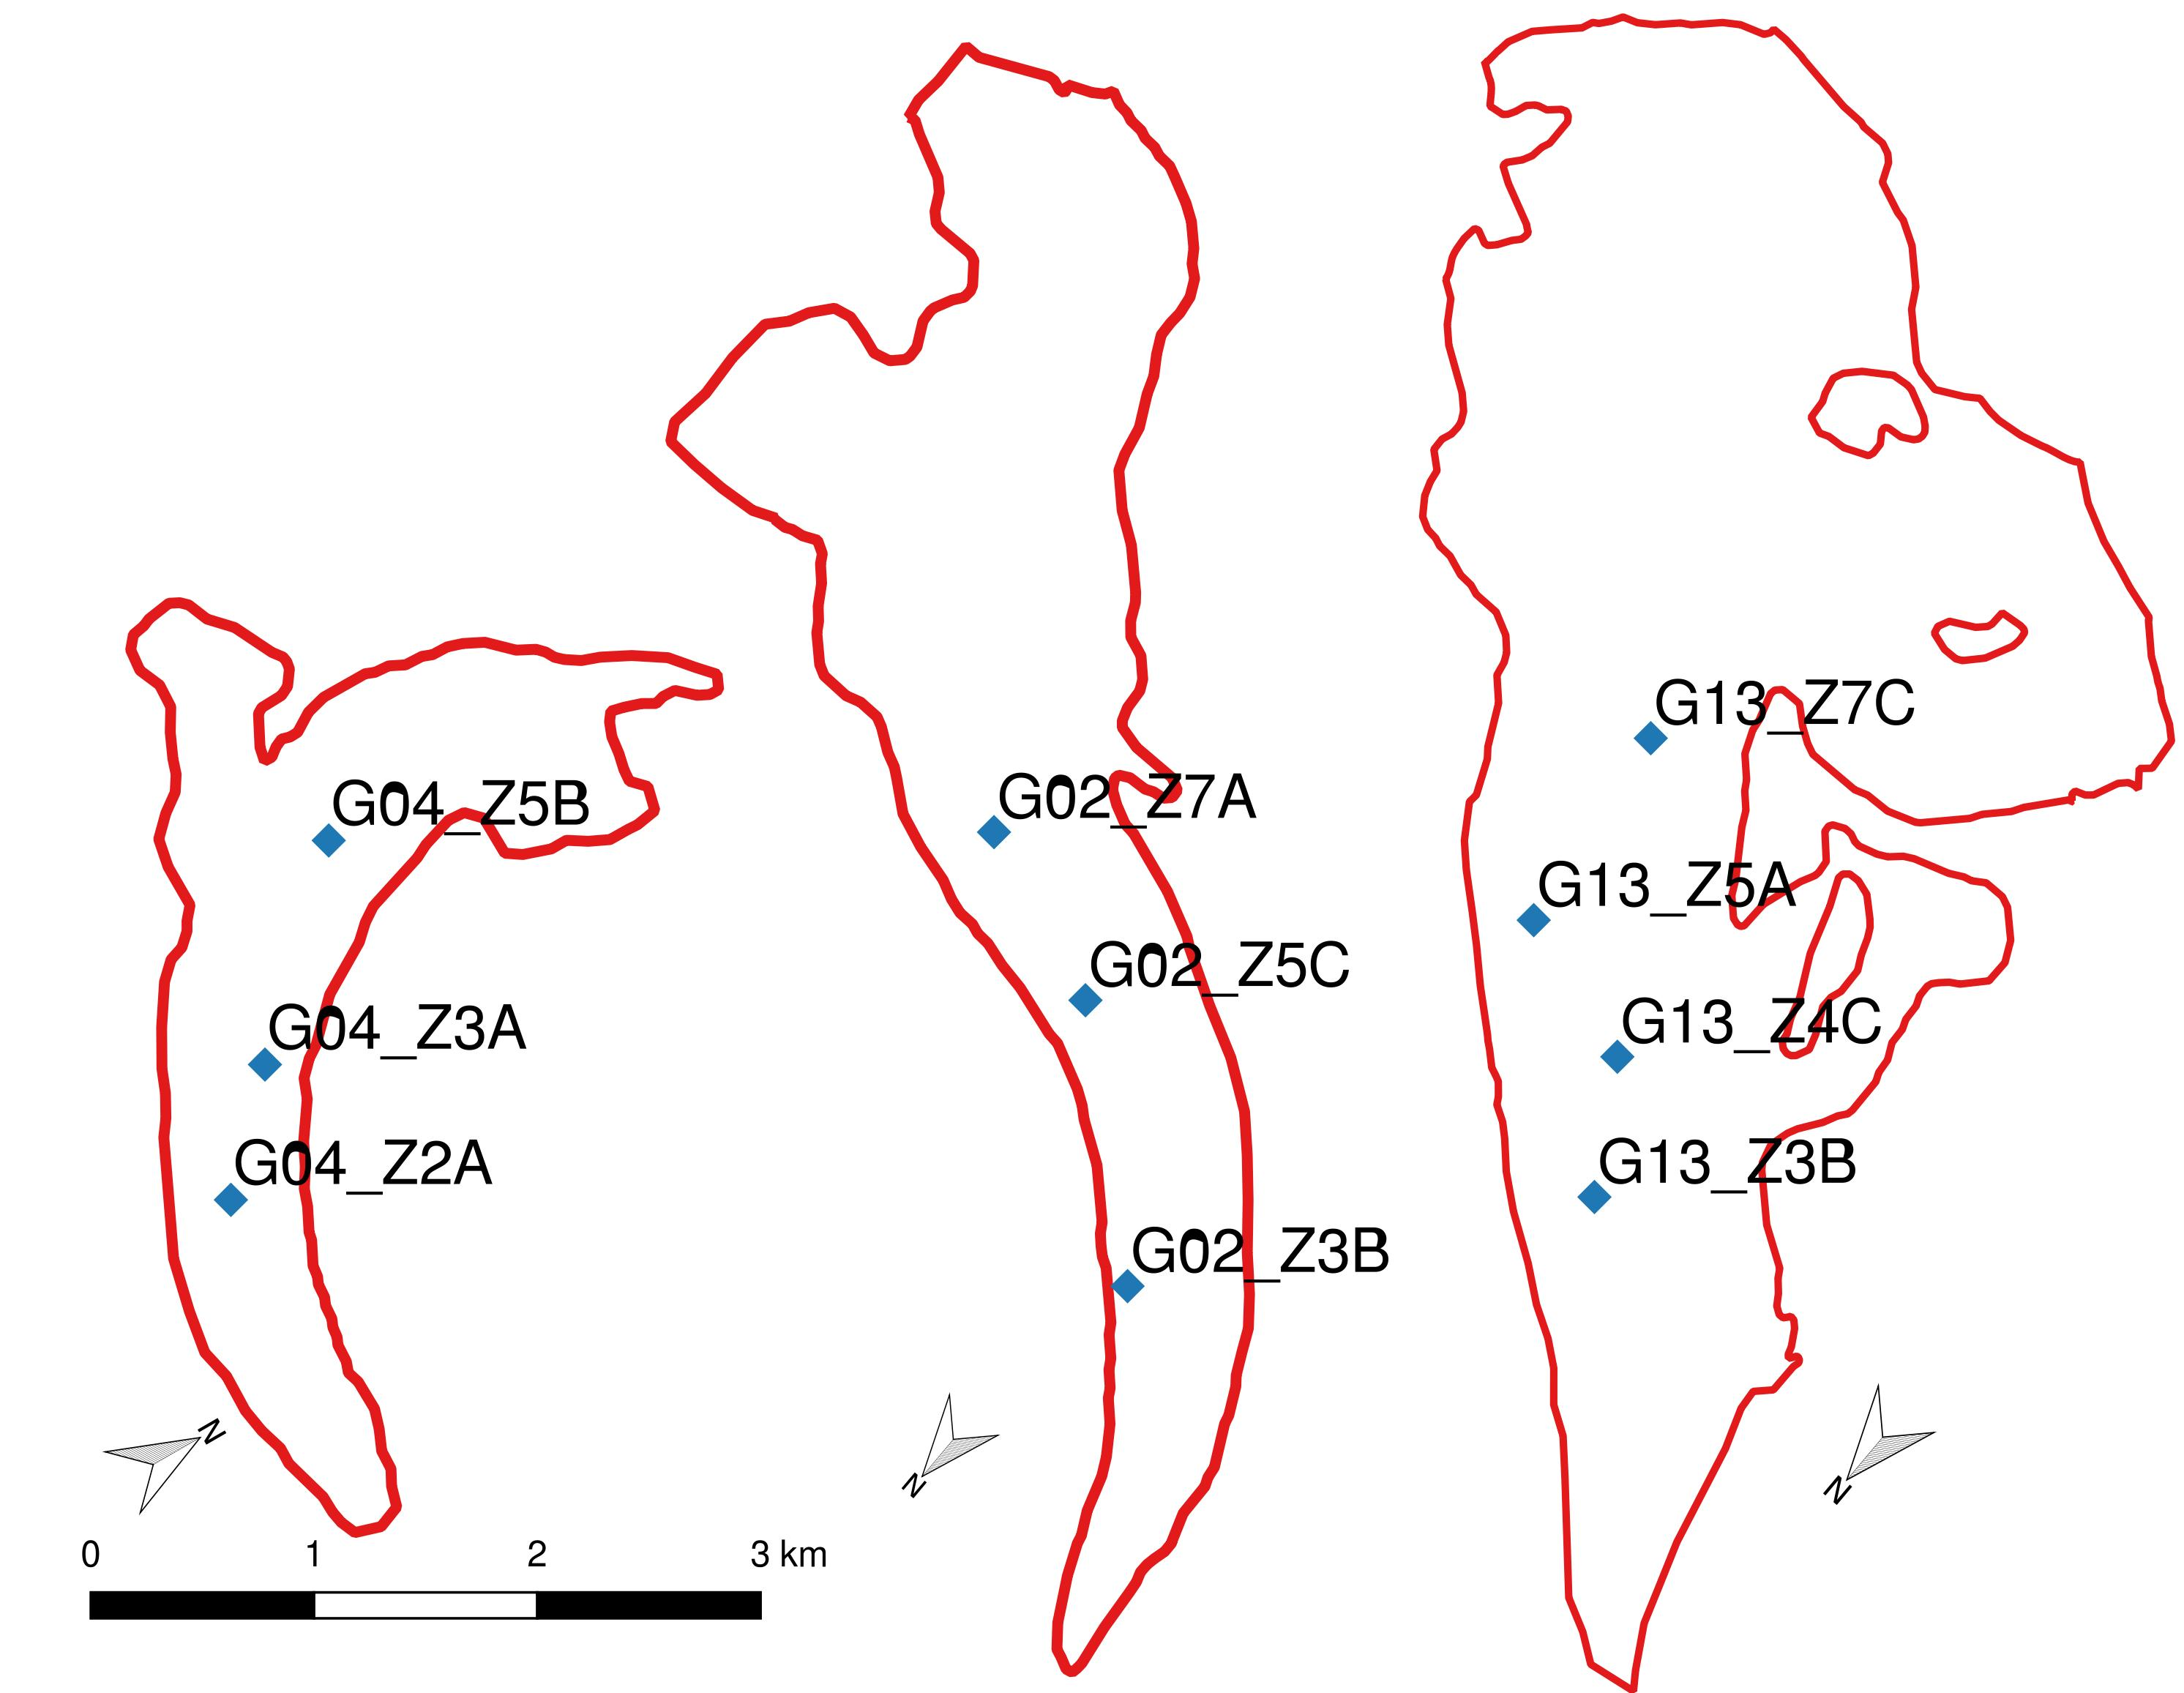
\includegraphics[width = 0.55\textwidth]{map_zigzaglocation_all.jpeg}\\
	\caption{Map of zigzag locations on Glaciers 4, 2 and 13 (left to right).}
	\label{fig:ZZ_locations}
\end{figure}

\begin{landscape}
\begin{figure}
	\centering
	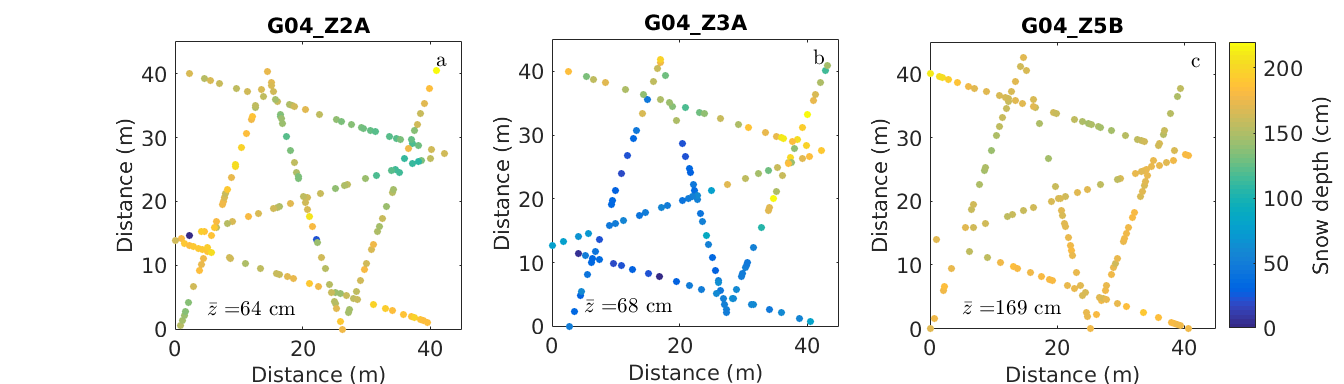
\includegraphics[width = 21 cm]{ZigzagDepth_G04.png}\\
	\caption{Snow depths measured in zigzags on Glacier 4. Mean depth ($\bar{z}$) is also reported. Zigzag elevations (left to right) are 2162, 2229 and 2360 m a.s.l. See Figure \ref{fig:ZZ_locations} for locations of each zigzag.}
	\label{fig:ZZ_G04}
\end{figure}

\begin{figure}
	\centering
	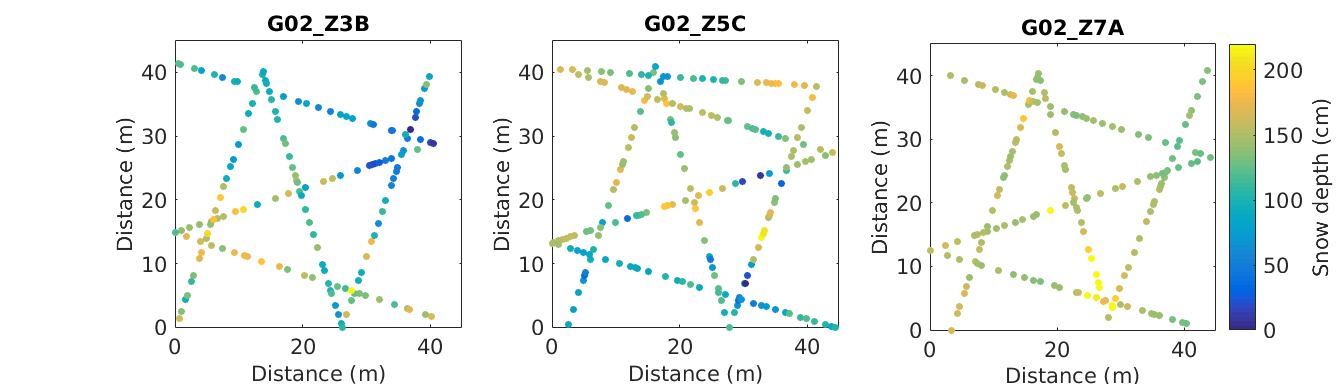
\includegraphics[width = 21 cm]{ZigzagDepth_G02.png}\\
	\caption{Snow depths measured in  zigzags on Glacier 2. Mean depth ($\bar{z}$) is also reported. Zigzag elevations (left to right) are 2172, 2332 and 2403 m a.s.l. See Figure \ref{fig:ZZ_locations} for locations of each zigzag.}
	\label{fig:ZZ_G02}
\end{figure}
\end{landscape}

\begin{figure}[H] 
	\centering
	 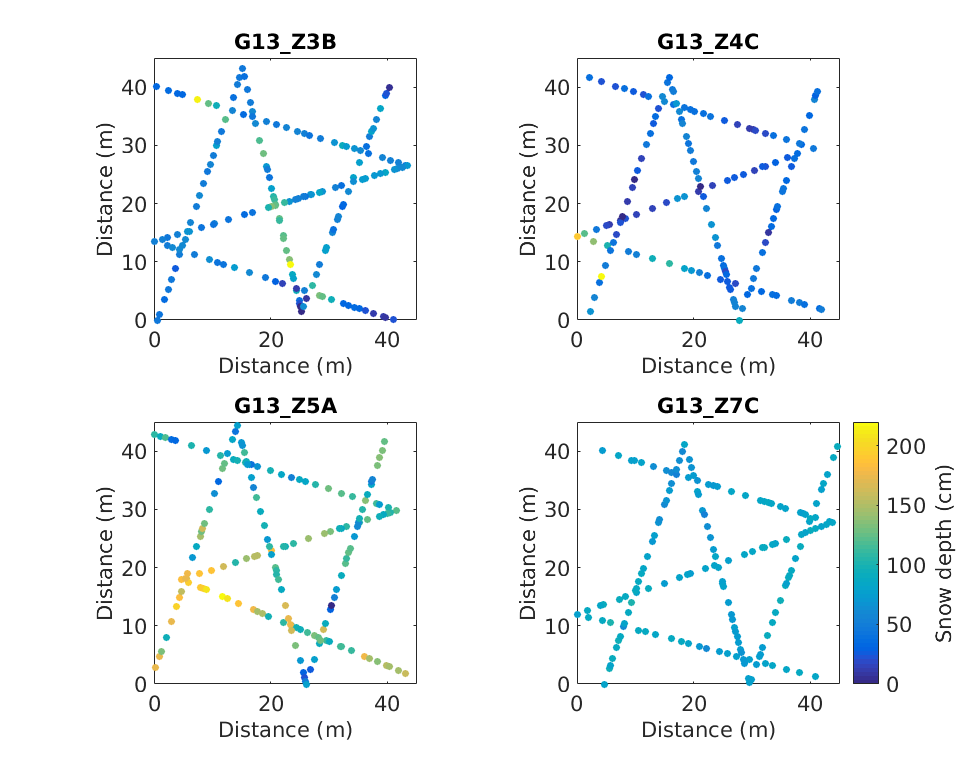
\includegraphics[width=0.9\textwidth]{ZigzagDepth_G13.png}%
	\caption{Snow depths measured in zigzags on Glacier 13. Mean depth ($\bar{z}$) is also reported. Zigzag elevations (a-d) are 2156, 2206, 2271 and 2297 m a.s.l. See Figure \ref{fig:ZZ_locations} for locations of each zigzag.}
	\label{fig:ZZ_G13}
\end{figure}


%%%%%%%%%%%%%%%%%%%%%%%%%%%%%%%%%%%%%%
\section{Snow water equivalent (SWE)}

Snow water equivalent (SWE) at sampling locations is estimated using eight density options (Section \ref{sec:density}). Estimates of SWE on each glacier are significantly different (Figure \ref{fig:AllSWEopts_boxplot}). Glacier 4 has two main groups of SWE estimates with a number of estimates that overlap (belong to group A and C). The estimate calculated using density F1 has a lower mean than the remaining estimates. Glacier 2 has four different grouping of SWE estimates but all estimates belong to multiple groups so there is no one estimate that differs from the rest. SWE estimates on Glacier 13 found using Federal Sampler-derived densities (Group B) have a higher mean SWE than those found using snowpit-derived densities (Groups A, C and D). The percent difference between the means of the SWE estimates are 12\%, 18\% and 19\%  for Glacier 4, 2 and 13, respectively. 

Density option 3 (Figures \ref{fig:SWEmap_S3} and \ref{fig:SWEmap_F3}), which uses a linear regression of density with elevation, is used in this study to examine how a regression based on topography could affect SWE estimates. Despite opposite relationships between density and elevation for Federal Sampler-derived densities and snowpit-derived densities (Table \ref{tab:elev_regress}), the SWE estimates do not differ significantly for Glaciers 4 and 2. On Glacier 13, these two SWE estimates do differ but all SWE estimates with density F differ from SWE estimates with density S. This systematic difference is perhaps a result of undersampling by the Federal Sampler on Glacier 13. Undersampling could have occurred because a considerable portion of the snowpack had undergone recent melt and snow depths were generally shallow, resulting in snow falling out of the sampling tube. 

For all density options, SWE is highest on Glacier 4 and lowest on Glacier 13. Glacier 4 also shows considerable SWE variability within the basin, with both high and low values along a single transect (Figures \ref{fig:SWEmap_S1} to \ref{fig:SWEmap_F4}). The lower, left side of Glacier 2 has low SWE with visible variability along transects. During field data collection, this area was observed to have dune-like ice features ($\sim$2 m) with alternating bare ice and wind-deposited snow patches.



\begin{figure}[H]
	\centering
	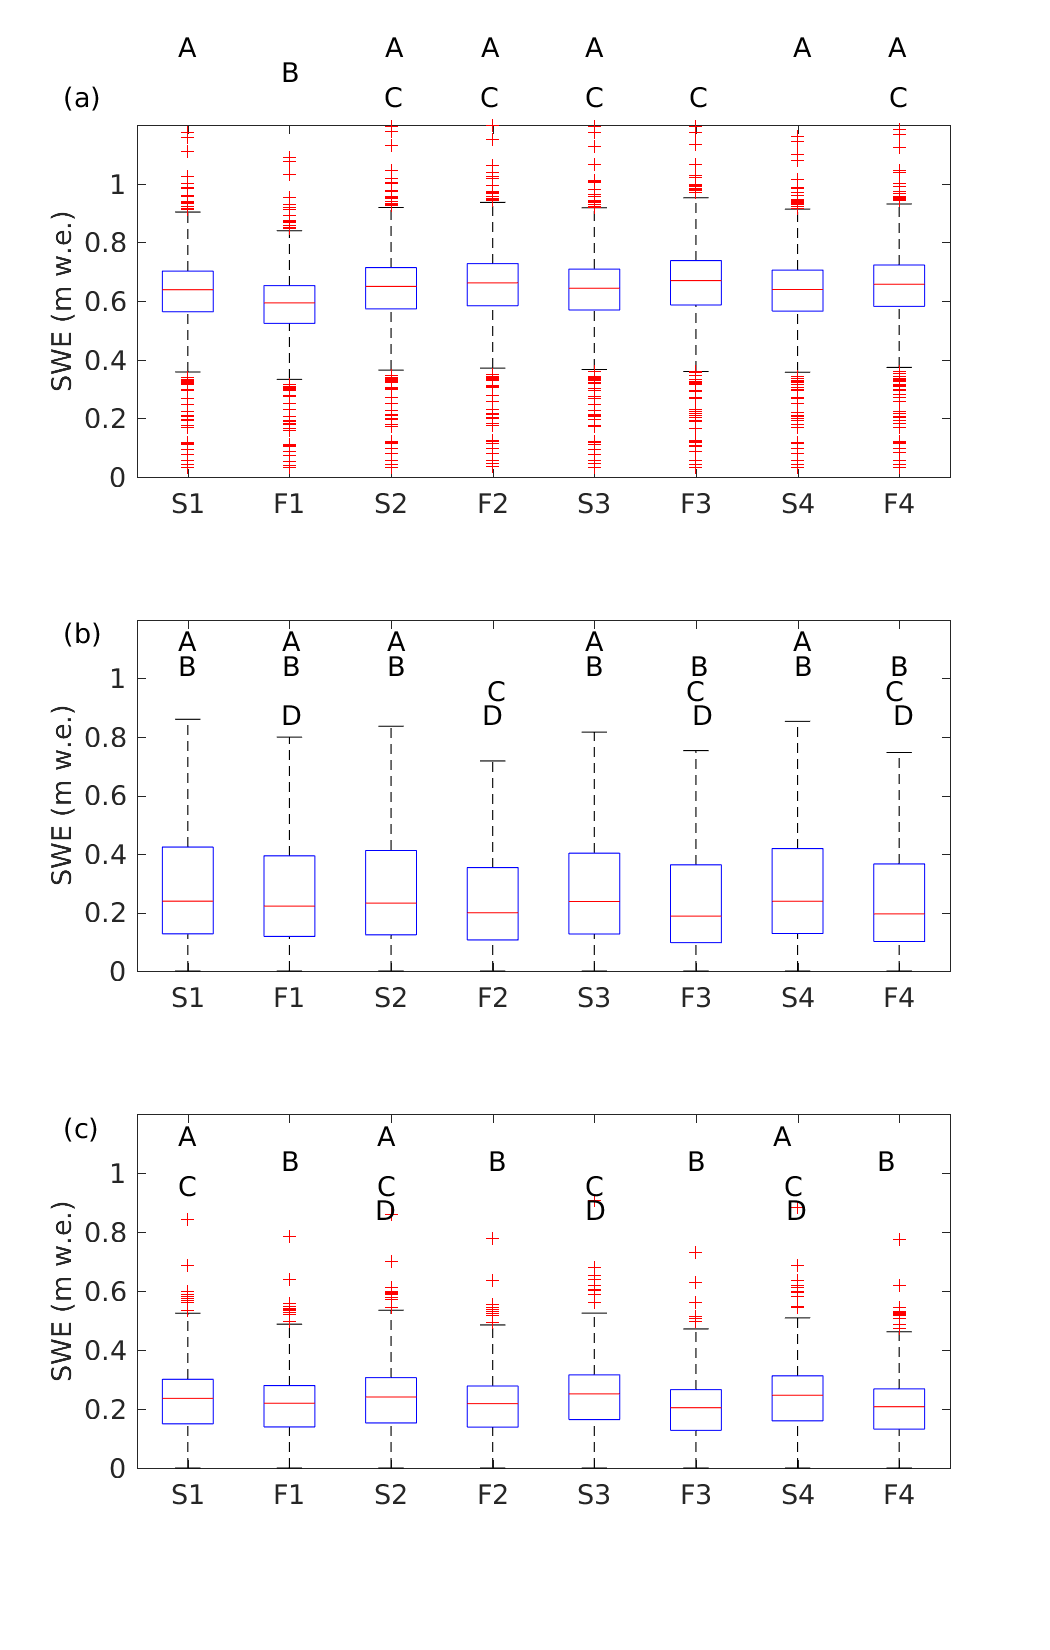
\includegraphics[height = 0.8\textheight]{AllSWEopts_boxplot.png}\\
	\caption{Boxplots of estimated SWE at sampling locations for Glacier 4 (a), Glacier 2 (b) and Glacier 13 (c). The density options using snowpit (S) or Federal Sampler (F) derived densities are mean from all glaciers (1), mean for individual glaciers (2), elevation regression (3) and inverse-distance weighting (4). SWE estimations using various density options were tested for differences using ANOVA (p$<$0.05). SWE estimates that were not significantly different for each glacier are labelled with the same letter (e.g. all estimates with A on Glacier 4 are significant different than all estimates with B).}
	\label{fig:AllSWEopts_boxplot}
\end{figure}


\begin{figure}[H]
	\centering
	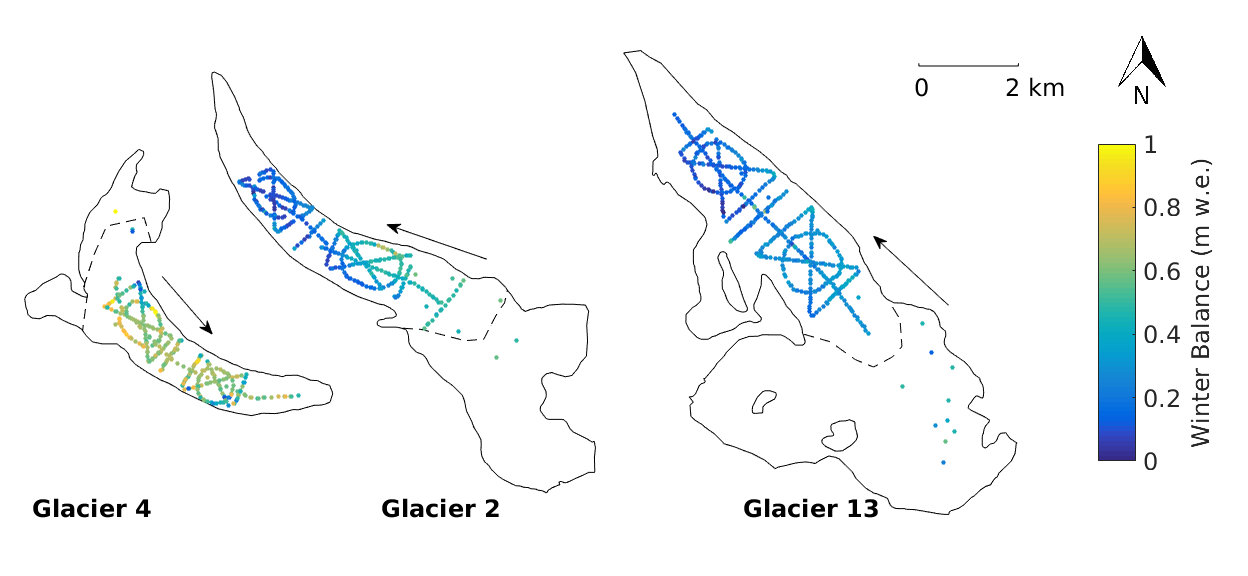
\includegraphics[width = \textwidth]{SWEmap_opt2.png}\\
	\caption{Estimated snow water equivalent (SWE) at measurement locations. Density was taken to be the mean value of all snowpit-derived densities from all glaciers (S1). Arrows show ice-flow direction and dashed lines show approximate ELA. Note that the individual measurement locations overlap on the figure.}
	\label{fig:SWEmap_S1}
\end{figure}

\begin{figure}[H]
	\centering
	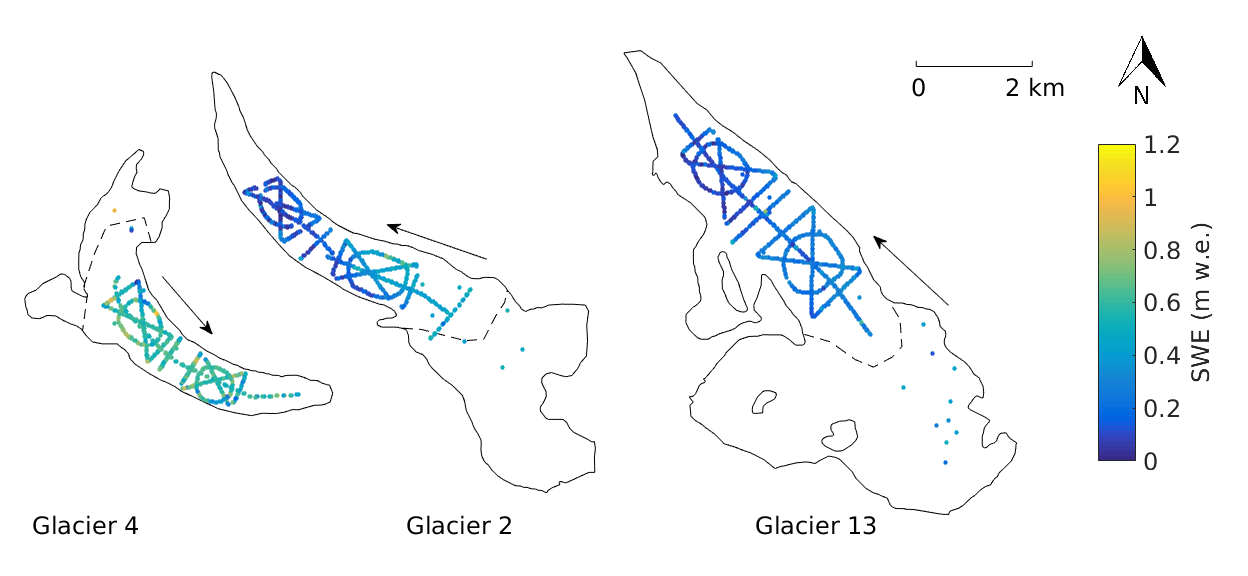
\includegraphics[width = \textwidth]{SWEmap_opt3.png}\\
	\caption{Estimated snow water equivalent (SWE) at measurement locations. Density was taken to be the mean value of all Federal Sampler-derived densities from all glaciers (F1). Arrows show ice-flow direction and dashed lines show approximate ELA. Note that the individual measurement locations overlap on the figure.}
	\label{fig:SWEmap_F1}
\end{figure}

\begin{figure}[H]
	\centering
	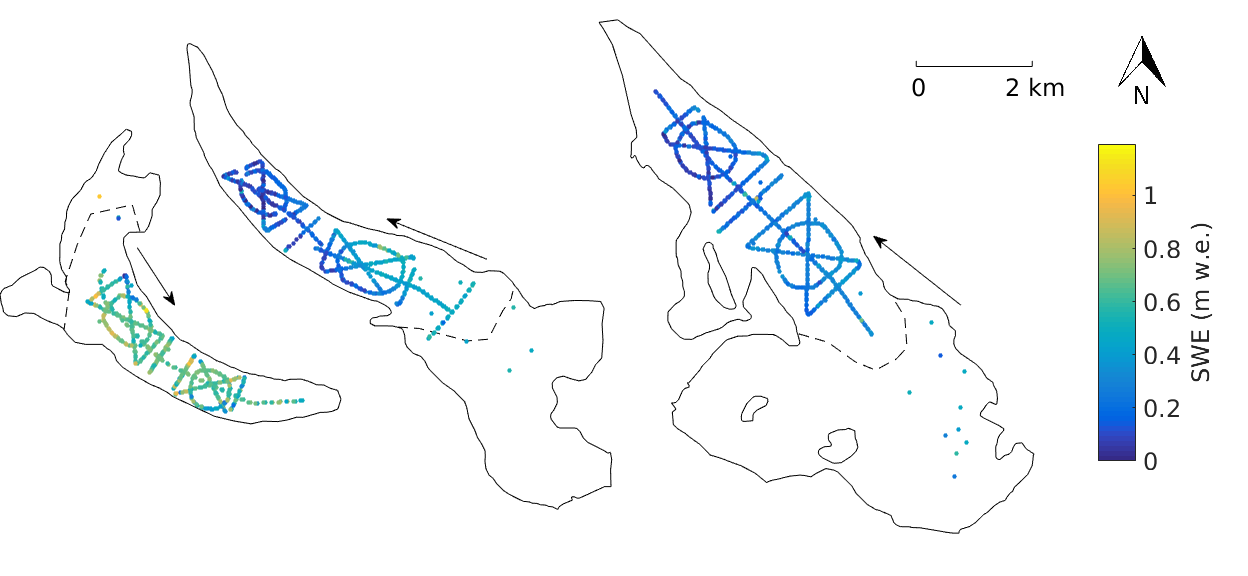
\includegraphics[width =\textwidth]{SWEmap_opt4.png}\\
	\caption{Estimated snow water equivalent (SWE) at measurement locations. Density for each glacier was taken to be the mean value of snowpit-derived densities from that glacier (S2). Arrows show ice-flow direction and dashed lines show approximate ELA. Note that the individual measurement locations overlap on the figure.}
	\label{fig:SWEmap_S2}
\end{figure}

\begin{figure}[H]
	\centering
	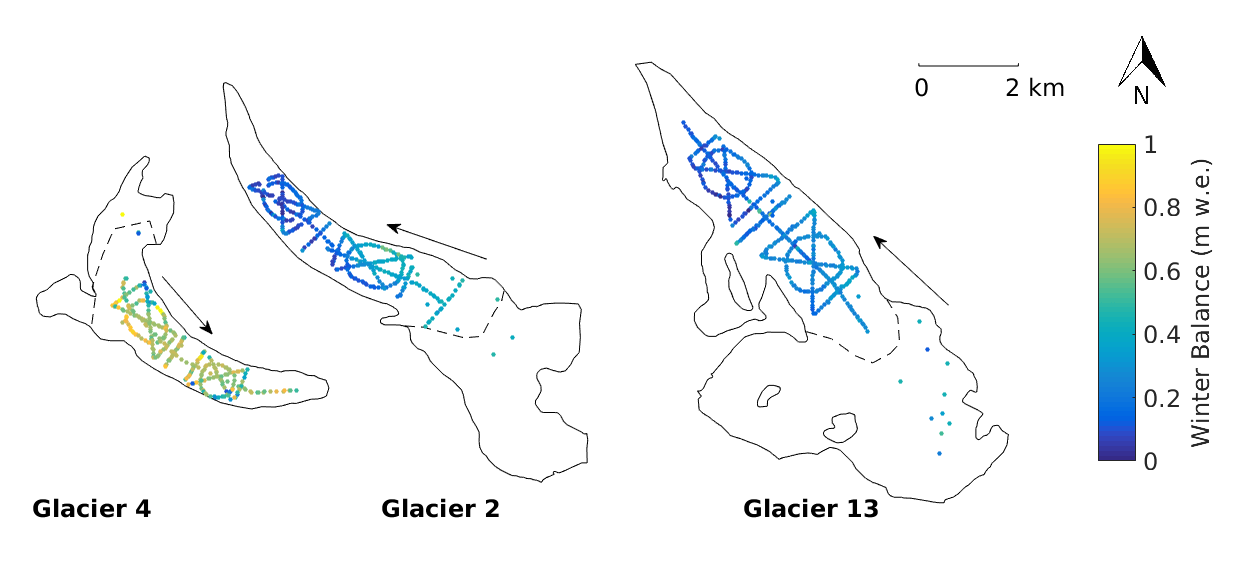
\includegraphics[width = \textwidth]{SWEmap_opt5.png}\\
	\caption{Estimated snow water equivalent (SWE) at measurement locations. Density for each glacier was taken to be the mean value of Federal Sampler-derived densities from that glacier (F2). Arrows show ice-flow direction and dashed lines show approximate ELA. Note that the individual measurement locations overlap on the figure.}
	\label{fig:SWEmap_F2}
\end{figure}

\begin{figure}[H]
	\centering
	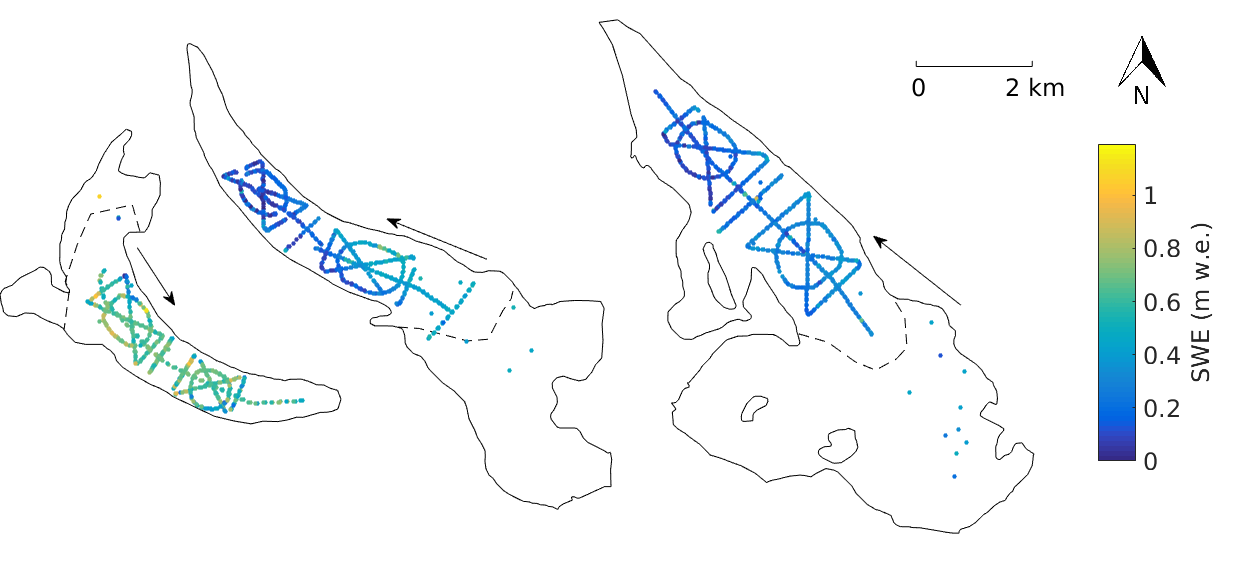
\includegraphics[width = \textwidth]{SWEmap_opt6.png}\\
	\caption{Estimated snow water equivalent (SWE) at measurement locations. Density was determined by using a linear fit between snowpit-derived density and elevation for each glacier (S3). Arrows show ice-flow direction and dashed lines show approximate ELA. Note that the individual measurement locations overlap on the figure.}
	\label{fig:SWEmap_S3}
\end{figure}

\begin{figure}[H]
	\centering
	\includegraphics[width = \textwidth]{SWEmap_opt7.png}\\
	\caption{Estimated snow water equivalent (SWE) at measurement locations.Density was determined by using a linear fit between Federal Sampler-derived density and elevation for each glacier (F3). Arrows show ice-flow direction and dashed lines show approximate ELA. Note that the individual measurement locations overlap on the figure.}
	\label{fig:SWEmap_F3}
\end{figure}

\begin{figure}[H]
	\centering
	\includegraphics[width = \textwidth]{SWEmap_opt8.png}\\
	\caption{Estimated snow water equivalent (SWE) at measurement locations. Density was calculated using inverse distance weighting using all snowpit-derived densities (S4). Arrows show ice-flow direction and dashed lines show approximate ELA. Note that the individual measurement locations overlap on the figure.}
	\label{fig:SWEmap_S4}
\end{figure}

\begin{figure}[H]
	\centering
	\includegraphics[width =\textwidth]{SWEmap_opt9.png}\\
	\caption{Estimated snow water equivalent (SWE) at measurement locations. Density was calculated using inverse distance weighting using all snowpit-derived densities (F4). Arrows show ice-flow direction and dashed lines show approximate ELA. Note that the individual measurement locations overlap on the figure.}
	\label{fig:SWEmap_F4}
\end{figure}


\chapter{Point scale results}



\begin{wraptable}[30]{R}{8cm}
\centering
\caption{Normality of data with various subgroups. $\chi^2$ values are shown and normally distributed data is bold ($p<0.05$). \transectAbb}
\label{tab:normality}
\begin{tabular}{cccc}
\textbf{Glacier} & \textbf{Transect} & \multicolumn{2}{c}{\textbf{$\chi^2$}} \\ 
\hline
\hline 
& LH & 14.9 &   \\
  & LC & 17.3 &   \\
  & LM & 6.6 &   \\
  & UH & 52.1 &   \\
  & UC & \textbf{5.9} &   \\
& UM & \textbf{1.4} &   \\
\multirow{-7}{*}{Glacier 4} & UT & 15.7 & \multirow{-7}{*}{ 115.4} \\ \hline
 & LH & 27.8 &  \\
 & LC & \textbf{5.0} &  \\
 & LM & \textbf{6.2} &  \\
 & UH & 43.8 &  \\
 & UC & 13.1 &  \\
 & UM & 31.3 &  \\
 & UT & \textbf{0.1} &  \\
\multirow{-8}{*}{Glacier 2} & BT & 13.1 & \multirow{-8}{*}{127.1} \\ \hline
  
  & LH & 32.1 &   \\ 
  
  & LC & 11.4 &   \\
  
  & LM & 18.1 &   \\
  
  & UH & 12.8 &   \\
  
  & UC & 17.6 &   \\
  
  & UM & 9.7 &   \\
  
\multirow{-7}{*}{ Glacier 13} & UT & 8.6 & \multirow{-7}{*}{ 39.4}
\end{tabular}
\end{wraptable}

\section{Point Scale}

This section details basic statistical results of the snow depth data at the point scale. The goal of these analyses is to examine variability of single measurements and to determine whether any correction need to be made to the collected data for future analysis. 

\subsection{Data normality}

A $\chi^2$ test is done to test whether the collected snow depth data are normally distributed. Generally, the transect snow depth data are not normally distributed and are even further from normality (larger $\chi^2$ values) for data grouped by glacier (Table \ref{tab:normality}). However, we chose to not transform the data in order to maintain its original context and because transformation of snow depth data is not typically done.  

\subsection{Observer differences}

An ANOVA for each transect of snow depth measurements taken by different observers shows that there are no differences between observers (p $>$ 0.05) (data not shown). The only exception is the Lower Hourglass on Glacier 4, where snow depth values collected by one observer were, on average, greater than the snow depth measurements taken by the other two observers ( AC$>$AP=CA with p $<$ 0.01). Since this was the first transect completed and the only one to show differences by observer, this difference can be considered an anomaly. This result shows that observer bias is likely to not affect the results of this study and no corrections to the data based on observer were applied.

\subsection{Standard deviation of snow depth along linear and curvilinear transects}

The mean standard deviation of snow depth measurements collected at each location within various transects was found by calculating the standard deviation of the three to four measurements made by each observer at each measurement location (Table \ref{tab:std_reproduce}. The mean of these standard deviations for each grouping (Table \ref{tab:std_reproduce}) represents the variability in snow depth for the sampling locations. It can be used to evaluate the representativeness of the mean snow depth values that were used in the analysis at larger scales.

The overall standard deviation of all measurements was calculated by taking all the depth measurements within a subset of the data and then calculating the standard deviation (Table \ref{tab:std_measure}). The overall standard deviation represents the variability in the depth field. 

The mean standard deviation varies between glaciers, transects, and observers but  generally, the reproducibility of depth measurement is on the order of centimetres (10$^0$). The overall standard deviation of measurements over the study area is on the order of 10$^1$. Therefore, the standard deviation of a snow depth measurement is small compared to the standard deviation of all snow depth measurements. When expressed as a percentage of the mean, the overall standard deviation (Table \ref{tab:std_measure}) is also larger than that of the mean standard deviation (Table \ref{tab:std_reproduce}). This shows that variability at the point scale (a single measurement location) is an order of magnitude smaller than the variability of the depth field for the length of a transect, so the use of the mean snow depth at each measurement location is a valid value to carry forward in the analysis. 

Variability in snow depth differs considerably between glaciers (Figure \ref{fig:box_depth}). Both the range and mean depth are largest for Glacier 4 and smallest for Glacier 13. Glacier 13 has the most outliers (\textgreater 1.5 $\times$ inner quartile range). The standard deviation of all measurement taken on a glacier (Table \ref{tab:std_measure}) is lowest for Glacier 13 and highest for Glacier 2, with the standard deviation of Glacier 4 being close to that of Glacier 2. 


\begin{wrapfigure}[22]{l}{0.7\textwidth} 
\centering
	\includegraphics[width = 0.7\textwidth]{box_depth.png}\\
	\caption{Variability in all snow depth measurements taken at each glacier. Red line indicates median, blue box shows first quantiles, bars indicate minimum and maximum values (excluding outliers), and red crosses show outliers, which are defined as being outside of the range of 1.5 times the quartiles (approximately $\pm2.7\sigma$).}
	\label{fig:box_depth}
\end{wrapfigure}

The standard deviation as a function of binned elevation show that the standard deviation decreases with elevation on both Glacier 2 and 13 but it increases with elevation on Glacier 4 (Figure \ref{fig:std_snowdepth_binned}). The regression of elevation and standard deviation as percent of the mean is strong for Glacier 2 (R$^2$ = 0.79) and weak for Glacier 13 (R$^2$ = 0.38) and Glacier 4 (R$^2$ = 0.12). Therefore, the variability is higher closer to the terminus of the Glacier 2 and there is no significant trend on Glacier 4 and 13. However, there are comparatively fewer depth measurements taken at higher elevations, which may skew the trend of higher variability close to the terminus. 

%% Std of reproducibility
\begin{table}[h]
\footnotesize
\centering
\caption{Mean standard deviation (cm) of snow depth measurements for the entire glacier (Overall Glacier), different transects (Overall Transect), and each observer. Standard deviation as a percent of the mean snow depth is shown in brackets. \transectAbb}
\label{tab:std_reproduce}
\begin{tabular}{cccccccc}
 &  &  &  & \multicolumn{4}{c}{\textbf{Observer}} \\
\multirow{-2}{*}{} & \multirow{-2}{*}{\textbf{Transect}} & \multirow{-2}{*}{\textbf{\begin{tabular}[c]{@{}c@{}}Overall \\ Glacier\end{tabular}}} & \multirow{-2}{*}{\textbf{\begin{tabular}[c]{@{}c@{}}Overall \\ Transect\end{tabular}}} & AP & GF & CA & AC \\ \hline \hline
  
  & LH &   & 5.1 (3\%)& 4.8  (3\%)& --- & 8.5 (5\%) & 2.0 (1\%) \\
  
  & LC &   & 4.7  (3\%)& 4.3  (3\%)& --- & 8.2  (5\%)& 1.7  (1\%)\\
  
  & LM &   & 3.7  (2\%)& --- & 4.7  (3\%)& 4.6  (2\%)& 1.9  (1\%)\\
  
  & UH &   & 2.6   (1\%)& 3.4   (1\%)& 2.2   (1\%)& --- & 2.3   (1\%)\\
  
  & UC &   & 1.9   (1\%)& 1.9   (2\%)& 2.3   (1\%)& --- & 1.5  (1\%) \\
  
  & UM &   & 1.9   (1\%)& --- & 1.7   (1\%)& 2.0 (1\%) & 2.0 (1\%)\\
  
\multirow{-7}{*}{ Glacier 4} & UT & \multirow{-7}{*}{ 3.5 (2\%)} & 3.9 (2\%)& 3.7 (2\%) & --- & 2.4 (1\%)& 5.6 (3\%)\\ \hline
 & LH &  & 5.4 (11\%)& 4.8 (9\%)& --- & 6.1 (13\%)& --- \\ 
 & LC &  & 5.0 (12\%)& 3.9 (11\%)& --- & 6.2 (15\%)& --- \\
 & LM &  & 6.5 (17\%)& --- & 6.8 (16\%)& 6.5 (18\%)& 6.0 (16\%)\\
 & UH &  & 4.1 (7\%)& 3.5 (5\%)& 4.4 (7\%)& 4.5 (9\%)& --- \\
 & UC &  & 7.0 (4\%)& 5.5 (3\%)& 7.0 (4\%)& 8.7 (4\%)& --- \\
 & UM &  & 4.2 (4\%)& 3.2 (3\%)& 5.2 (4\%)& 4.1 (4\%)& --- \\
 & UT &  & 5.6 (10\%)& 3.2 (6\%)& --- & 8.2 (13\%)& --- \\
\multirow{-8}{*}{Glacier 2} & BT & \multirow{-8}{*}{5.1 (7\%)} & 2.2 (2\%)& 2.2 (2\%)& --- & 3.0 (2\%)& 1.5 (1\%) \\ \hline
  
  & LH &   & 3.8 (10\%)& 3.1 (6\%)& 4.1 (12\%) & 4.0 (13\%)& --- \\ 
  
  & LC &   & 4.5 (8\%)& 2.9 (6\%)& 4.8 (9\%)& 5.8 (8\%)& --- \\
  
  & LM &   & 6.6 (13\%)& 4.6 (10\%)& 7.7 (16\%)& 7.6 (14\%)& --- \\
  
  & UH &   & 3.5 (4\%)& 3.4 (4\%)& 3.6 (5\%)& 3.4 (5\%)& --- \\
  
  & UC &   & 3.8 (4\%)& 3.4 (4\%)& 4.0 (4\%)& 4.0 (4\%)& --- \\
  
  & UM &   & 4.8 (6\%)& 4.4 (5\%)& 5.8 (7\%) & 4.4 (5\%) & --- \\
  
\multirow{-7}{*}{ Glacier 13} & UT & \multirow{-7}{*}{ 4.2 (6\%)} & 4.1 (6\%)& 2.7 (4\%)& 4.8 (6\%)& 4.6 (7\%)& ---
\end{tabular}
\end{table}


%% Std of measurement
\begin{table}[]
\footnotesize
\centering
\caption{Overall standard deviation (cm) of snow depth measurements for the entire glacier (Overall Glacier), different transects (Overall Transect), and each observer. Standard deviation as a percent of the mean snow depth is shown in brackets. \transectAbb The standard deviation of all transect data was 64.6 cm.}
\label{tab:std_measure}
\begin{tabular}{cccccccc}
 &  &  &  & \multicolumn{4}{l}{\textbf{Person}} \\
\multirow{-2}{*}{\textbf{Glacier}} & \multirow{-2}{*}{\textbf{Pattern}} & \multirow{-2}{*}{\textbf{\begin{tabular}[c]{@{}l@{}}Overall \\ Glacier\end{tabular}}} & \multirow{-2}{*}{\textbf{\begin{tabular}[c]{@{}l@{}}Overall \\ Pattern\end{tabular}}} & AP & GF & CA & AC \\ \hline \hline
  
  & LH &   & 51.3  (28\%)& 51.4  (29\%) & --- & 54.8  (32\%) & 45.7  (24\%) \\
  
  & LC &   & 45.2  (26\%) & 50.5  (30\%) & --- & 44.1  (25\%) & 39.8  (23\%) \\
  
  & LM &   & 27.2  (15\%) & --- & 21.6   (11\%)& 36.3  (19\%) & 22.5  (12\%) \\
  
  & UH &   & 48.5  (28\%) & 48.6  (28\%) & 51.2   (29\%)& --- & 45.8  (27\%) \\
  
  & UC &   & 44.2  (23\%) & 44.8  (23\%) & 38.2   (21\%)& --- & 48.2   (26\%)\\
  
  & UM &   & 22.5  (13\%) & --- & 24.1  (14\%) & 20.7  (12\%) & 22.7  (13\%) \\
  
\multirow{-7}{*}{ Glacier 4} & UT & \multirow{-7}{*}{ 44.7  (25\%)} & 26.0   (13\%)& 25.1  (13\%) & --- & 25.1  (13\%) & 27.7  (14\%) \\ \hline
 & LH &  & 29.9  (67\%) & 29.2  (63\%) & --- & 30.6  (71\%) & --- \\
 & LC &  & 29.3  (61\%) & 28.6  (63\%) & --- & 30.1  (59\%) & --- \\
 & LM &  & 18.4  (43\%) & --- & 20.8   (45\%)& 15.5  (39\%) & 18.1  (43\%) \\
 & UH &  & 42.0  (39\%) & 39.1  (37\%) & 41.6  (38\%) & 45.6  (42\%) & --- \\
 & UC &  & 55.0   (52\%)& 55.3  (53\%) & 55.2  (52\%) & 56.1  (52\%) & --- \\
 & UM &  & 35.1  (29\%) & 38.4  (33\%) & 34.5  (29\%) & 31.8  (27\%) & --- \\
 & UT &  & 36.4  (61\%) & 27.3 (51\%) & --- & 43.9  (70\%) & --- \\
\multirow{-8}{*}{Glacier 2} & BT & \multirow{-8}{*}{49.3 (62\%)} & 20.8 (14\%)& 13.8 (10\%)& --- & 13.7 (9\%) & 30.4 (22\%) \\ \hline
  
  & LH &   & 27.4  (56\%) & 25.7 (53\%) & 27.5 (58\%) & 28.9 (57\%) & --- \\
  
  & LC &   & 27.1  (59\%) & 25.8 (57\%) & 21.4 (52\%) & 32.6 (68\%) & --- \\
  
  & LM &   & 24.9  (52\%) & 22.8 (60\%) & 27.5 (56\%) & 23.6 (42\%) & --- \\
  
  & UH &   & 21.0  (25\%) & 21.1 (25\%) & 21.4 (25\%) & 20.4 (24\%) & --- \\
  
  & UC &   & 16.3  (18\%) & 17.6 (21\%) & 14.5 (16\%) & 16.6 (18\%) & --- \\
  
  & UM &   & 29.4  34(\%) & 26.6 (32\%) & 33.4 (39\%) & 28.0 (33\%) & --- \\
  
\multirow{-7}{*}{ Glacier 13} & UT & \multirow{-7}{*}{ 30.5 (46\%)} & 32.7 (50\%) & 21.5 (31\%) & 44.4 (63\%) & 26.4 (42\%) & ---
\end{tabular}
\end{table}


\begin{figure}
    \centering
    \begin{subfigure}[b]{0.8\textwidth}
        \includegraphics[width=\textwidth]{binned_std.png}
        \caption{}
    \end{subfigure}
    
    \begin{subfigure}[b]{0.8\textwidth}
        \includegraphics[width=\textwidth]{binned_std_percent.png}
        \caption{}
    \end{subfigure}

    \caption{Standard deviation (a) and standard deviation as percent of mean (b) of all snow depth measurements binned in elevation bands of 10 m. Bars at the top of the figure indicate the elevation ranges of the three study glaciers. The regression of elevation and standard deviation of snow depth is shown as a coloured line within the data.}
    \label{fig:std_snowdepth_binned}
\end{figure}



%   BACK MATTER  %%%%%%%%%%%%%%%%%%%%%%%%%%%%%%%%%%%%%%%%%%%%%%%%%%%%%%%%%%%%%%
%
%   References and appendices. Appendices come after the bibliography and
%   should be in the order that they are referred to in the text.
%
%   If you include figures, etc. in an appendix, be sure to use
%
%       \caption[]{...}
%
%   to make sure they are not listed in the List of Figures.
%

\backmatter%
	\addtoToC{Bibliography}
	\bibliographystyle{plain}
	\bibliography{/home/glaciology1/Documents/MastersDocuments/MastersLit}

\begin{appendices} % optional
	\chapter{GPS Waypoint Creation and Upload to GPS Device}
	
	To create the desired \textbf{transect} waypoints and enter them into the handheld GPS devices (Garmin GPSMAP 64s) the following steps were taken:
\begin{enumerate}
\item In QGIS, the outline of the glacier was selected from the Randolph Glacier Inventory (RGI 5.0) \citep{Pfeffer2014} and a recent, end-of-summer Landsat image was downloaded (LC80620172013248LGN00 image courtesy of the U.S. Geological Survey). 
\item The ELA was estimated by tracing out the snow line from the Landsat image.
\item The desired transects were traced out in QGIS within the intended area. The tool `QChainage' was then used to divide the line into points that were spaced every 30 m. Note that the shape file of the transect lines was projected into UTM coordinates to space points using units of metres. 
\item The new point file was then saved as a comma-separated value file (`.csv') and opened in Excel. Note that the projection of the file was WGS84 so that the exported file had latitude and longitude values, which were needed for the GPS software.
\item The points were then named according to their location, area, transect, and point order. A column was made for `Glacier' and `Transect' and filled in for each point (using the drag function in Excel). This required identifying the range of points in QGIS (which were numbered) that corresponded to each transect and relating them to the numbered points in the Excel file (this was a bit cumbersome). The two columns were then combined and a sequential number added to the end. This column requires the header 'name' to be correctly identified as the name of the point in the GPS software.
\item The file with the point names was then imported into to the Garmin software \textit{BaseCamp} and the waypoints were transferred to the GPS devices using this software. 
\end{enumerate}

To create the desired \textbf{zigzag} waypoints and enter them into the GPS devices the following steps were taken:
\begin{enumerate}
\item As described above, the outline of the glacier was selected from the RGI and a recent, end-of-summer Landsat image was downloaded. The ELA was estimated by tracing out the snow line from the Landsat image.
\item The ablation area was then divided into 7 zones that had approximately equal area (estimated by eye) and a polygon was traced out for each zone (within one shape file). 
\item In QGIS, the tool `Random Points' was then used to choose three random locations in each polygon. This was the location of the SWE measurements A, B, and C in each zone. 
\item The file with the SWE measurement locations was saved as a `.csv'. The points were then named in Excel and exported to the GPS device as described above.
\item A new shape file was then created for the vertices of the zigzag. The vertices were created (in sequential order) so that they fit along the edges of one cell of the SPOT5 DEM. This was done by actually looking at one cell and placing the points along the edges at the intended locations. As a result, the SWE measurement location within the zigzag was not the same between zigzags. 
\item Once all the zigzag point groups were created, the file was saved as a `.csv', points named accordingly, and then exported to the GPS device as described above. 
\end{enumerate}

The locations of snowpits and snow cores were chosen by hand in a separate shape file. This file was then saved as a `.csv', the points named, and the file exported to the GPS devices as described above. 

The files that had the names of the points were then imported back into QGIS so that the maps with point labels could be created.  Since the order of completing measurements was determined in the field, these maps helped to quickly decide on the most efficient plan because they aided in determining the relative location of zigzags and transects.


%%%

\chapter{Field Maps}


\noindent \large{\textbf{Glacier 4}}\\
\fbox{\includegraphics[height = 0.45\textheight]{G04_Topo.jpeg}}\\
\fbox{\includegraphics[height = 0.45\textheight]{G04_Overview.jpeg}}\\
\fbox{\includegraphics[height = 0.45\textheight]{G04_ZZ.jpeg}}\\
\fbox{\includegraphics[height = 0.45\textheight]{G04_LH.jpeg}}\\
\fbox{\includegraphics[height = 0.45\textheight]{G04_LH.jpeg}}\\
\fbox{\includegraphics[height = 0.45\textheight]{G04_UH.jpeg}}\\
\fbox{\includegraphics[height = 0.45\textheight]{G04_M.jpeg}}\\
\fbox{\includegraphics[height = 0.45\textheight]{G04_A.jpeg}}\\

\pagebreak
\noindent \large{\textbf{Glacier 2}}\\
\fbox{\includegraphics[height = 0.45\textheight]{G02_topo.jpeg}}\\
\fbox{\includegraphics[height = 0.45\textheight]{G02_Overview.jpeg}}\\
\fbox{\includegraphics[height = 0.45\textheight]{G02_ZZ.jpeg}}\\
\fbox{\includegraphics[height = 0.45\textheight]{G02_LH.jpeg}}\\
\fbox{\includegraphics[height = 0.45\textheight]{G02_LH.jpeg}}\\
\fbox{\includegraphics[height = 0.45\textheight]{G02_UH.jpeg}}\\
\fbox{\includegraphics[height = 0.45\textheight]{G02_M.jpeg}}\\
\fbox{\includegraphics[height = 0.45\textheight]{G02_A.jpeg}}\\

\pagebreak
\noindent \large{\textbf{Glacier 13}}\\
\fbox{\includegraphics[height = 0.45\textheight]{G13_Topo.jpeg}}\\
\fbox{\includegraphics[height = 0.45\textheight]{G13_Overview.jpeg}}\\
\fbox{\includegraphics[height = 0.45\textheight]{G13_ZZ.jpeg}}\\
\fbox{\includegraphics[height = 0.45\textheight]{G13_LH.jpeg}}\\
\fbox{\includegraphics[height = 0.45\textheight]{G13_LH.jpeg}}\\
\fbox{\includegraphics[height = 0.45\textheight]{G13_UH.jpeg}}\\
\fbox{\includegraphics[height = 0.45\textheight]{G13_M.jpeg}}\\
\fbox{\includegraphics[height = 0.45\textheight]{G13_A.jpeg}}\\


%%%%
\chapter{Data Processing Scripts}

Converting snow depth and density measurements to usable values of snow water equivalent (SWE) is done using a number of scripts written in Matlab. Since there are a number of possible variations for how SWE is estimated, various options are outlined in the `OPTIONS.m' script. To run the entire data processing framework first ensure your desired SWE estimation options are reflected in the `OPTIONS.m' script and then run both `OPTIONS.m' and `MAIN.m'

\section{Snow depth measured with graduated avalanche probe}
\subsection{Linear and curvilinear transect surveys}
\label{app:transect_calc}

 The following methodology was used to determine measurement locations along transects (each step corresponds with a section of the Matlab code `MeasurementLocations.m'): 
\begin{enumerate}
	\item Waypoint (WP) locations were exported from the GPS units using the Garmin BaseCamp program. They were then imported to QGIS and exported with UTM coordinates in the file `GlacierWP\_UTM.xlsx'. 
	\item In order to obtain the measurement locations for the first WPs of each pattern, a fictitious WP was created that was along the line between the first and second WPs, but located ahead of the first WP. These fictitious waypoints were then inserted into the original data. 
	\item A set of 1000 equally spaced points was created along a straight line between each set of subsequent of WPs (including the fictitious WPs from the previous step) using the function linspaceNDim.m created by Steeve Ambroise and downloaded from the MathWorks File Exchange. The Euclidean distance between these interpolated points and the marked WP was then calculated and the points with distances closest to the assumed separation between observers were retained. A matrix was then created, which has the UTM Zone 7N Easting and Northing of each measurement location and is labelled with the marked WP and a decimal that corresponds to the relative observer (e.g. label 45.2 means that the location was determined from the marked WP \#45 and is 20 m behind this WP because it is the second observer). 
\end{enumerate}

Data recorded by each observer in the field books were entered into a spreadsheet format and then imported and processed in Matlab according to the following steps (each step corresponds with a section of the Matlab code `Import\_Transect.m'):
\begin{enumerate}
	\item A spreadsheet was created with a sheet for data from each snow depth (SD) field book (SD\#1, SD\#2, SD\#3, and SWEDepth). For each reference WP there were values for all snow depth measurements and their quality (1 for good, 0 for bad or uncertain), written comments, field book name, glacier number, observer, transect, and date collected.  
	\item The quality, comments, book name, glacier name, observer, pattern, and date entries were turned into categorical variables (data type in Matlab), allowing for efficient grouping and data searching in future analysis.
	\item Each depth measurement was then assigned the corresponding measurement location UTM from the `MeasurementLocations.m' script. This was done by matching the WP number from the field books and that of the marked WPs and then assigning the coordinates from the WP ending with .1 to depths recorded in book SD\#1, and likewise for the remaining books. The data sets from each field book were then made to be the same dimensions by inserting empty cells for WPs where no data were recorded in that set of observations. 
	\item The data were then arranged in a structure variable (called SD) with rows corresponding to each book (e.g. row 1 is data from book SD\#1) and columns corresponding to the various types of data (e.g. depth values or glacier name). For example, the matrix with the glacier name for each value recorded in the book SD\#1 can be accessed with `SD(1).glacier'.
\end{enumerate}

Subsets of the transect data can be pulled using the function `pulldata.m'. The function is called with \texttt{pulldata(data, book, glacier, person, pattern, quality, format)}. Here, \texttt{data} is the full SD structure, \texttt{book, glacier, person, and pattern} are all strings that refer to desired categories, \texttt{quality} differentiates between good (1), bad (0), or `all' data, and \texttt{format} specifies the formatting of the full depth matrix as being either a column vector (`skinny') or a matrix with depth values for one WP in a single row. 

\subsection{Zigzag surveys}

Data from zigzag surveys, which include the measured snow depths and distances between adjacent measurement points, were entered to a spreadsheet. The data were then processed using the following procedure (each step corresponds with a section of the Matlab code `Import\_Zigzag.m'):
\begin{enumerate}
\item Data were imported into Matlab.
\item Categorical data, including glacier number, zigzag zone label, reference vertex, data quality, observer name, date collected, and book name, were created.
\item A structure that contained the depth data and categorical variables was created.
\item The distance of each measurement point from its reference vertex was then calculated (Figure \ref{fig:zigzag_location_options}). These locations were assumed to be a cumulative sum of distances in a straight line between two subsequent vertices. Two options exist for determining the location of the reference vertex:
 	\begin{enumerate}
	\item Option 1 calculates the distance of each point from the UTM coordinates of the reference vertex.
	\item Option 2 calculates the distance of each point from the end of the previous line of measurements. The coordinates of the vertices were used for the start of each `Z' shape (ZZ01 and ZZ05).
	\end{enumerate}
\item The final processing removes poor quality data and converts snow depth to snow water equivalent (SWE) based on the density calculated from the average SWE values measured with the Federal Sampler in each zigzag (see Section \ref{sec:density}).
\end{enumerate}

\section{Snow density}

Snow density data were first entered into and organized in a spreadsheet then processed in Matlab as follows (each step corresponds with a section of the Matlab code `Import\_Density.m'): 
\begin{enumerate}
\item Snow density data were imported into Matlab and poor quality data were removed. 
\item Snowpit-derived snow density values were assigned to their respective location names and coordinates.
\item For each zigzag survey, the mean snow density (Federal Sampler), snow density standard deviation, and number of good quality measurements were calculated.
\item For remaining Federal Sampler measurement locations, the mean snow density, snow density standard deviation, and number of good quality measurements were calculated. 
\item A structure with the processed data was created (\texttt{Density}).
\end{enumerate}

The final version of the \texttt{Density} structure includes five fields:
\begin{itemize}
\item[]\texttt{Density.snowpit} contains snow density data from snowpits. Columns correspond to snowpit label, integrated density, Easting, Northing, elevation, minimum density, maximum density, snow depth.
\item[]\texttt{Density.pitANDtube} includes data from locations where measurements were taken in a snowpit and with a Federal Sampler. Columns correspond to snowpit label, Federal  Sampler mean density, standard deviation, minimum Federal Sampler-derived density, maximum Federal Sampler-derived density, number of observations, snowpit-derived density, site elevation, minimum snowpit density, and maximum snowpit density.
\item[]\texttt{Density.tube} includes Federal Sampler data. Columns correspond to location label, density mean, standard deviation, minimum and maximum, number of good quality observations, Easting, Northing, elevation, and snow depth. 
\item[]\texttt{Density.zigzagtube} includes density values at each zigzag location estimated using a Federal Sampler. Columns correspond to zigzag label, mean density, standard deviation, number of observation, and site elevation. 
\item[]\texttt{Density.SWEdepth} is a summary of all the Federal Sampler derived density data and corresponding snow depth measurements. Columns correspond to location label, mean probe depth, depth measured by the Sampler, and snow density measured using the Federal Sampler. 
\end{itemize}

\section{Snow water equivalent (SWE)}

The final SWE values for each measurement location are calculated in Matlab using the following steps (this corresponds to the script `Import\_SWE.m'):
\begin{enumerate}
\item The desired density interpolation method is selected in the `OPTIONS.m' script.
\item Snow depth values from transects, zigzags, and extra measurements is complied into a single structure called `SWE'.
\item The elevation of each measurement location according to the SPOT5 DEM was found in QGIS and the elevations are imported to Matlab and assigned to their respective depth measurement values.
\item The density values for each snow depth measurement location were estimated according to the chosen method. SWE was then calculated. 
\end{enumerate}
To select the desired density calculation option (or to cycle through all options), change the value of \texttt{options.DensitySWE} to the appropriate option number.

The final version the \texttt{SWE} structure includes three rows, which correspond to Glacier 4, 2, and 13, and ten fields. The fields are: 
\begin{itemize}
\item \texttt{book} (field book where measurement is written)
\item \texttt{comments} (any comments noted by observer)
\item \texttt{density} (the density value used to calculate SWE)
\item \texttt{depth} (mean depth measured at each sampling location, $n=3$ usually)
\item \texttt{glacier} (glacier number where measurement was taken)
\item \texttt{label} (measurement point reference label; for transects this is the waypoint number and relative position, for other measurements this is a label associated with transect and location)
\item \texttt{pattern} (transect, or set of transects, that include the measurement)
\item \texttt{person} (initials of observer)
\item \texttt{swe} (estimated SWE value)
\item \texttt{utm} (the Easting and Northing for the measurement location as well as the DEM elevation). 
\end{itemize}
For example, to access the SWE values for Glacier 2, one would type \texttt{SWE(2).swe}. 

The \texttt{SWE} structure includes all data that is collected for each glacier. If there is a need to remove the zigzag data or keep only the zigzag data, the script `ZigzagRemoval.m' can be run. Set the option for including or excluding zigzag data in the script `OPTIONS.m'.









\end{appendices}
\end{document}
